\documentclass[a4paper]{llncs}

\usepackage{alltt}
\usepackage{amssymb}
\usepackage{caption}
\usepackage{paralist}
\usepackage{nicefrac}
\usepackage{booktabs}
\usepackage{xspace}
\usepackage{amsmath}
\usepackage{marvosym}
\usepackage{wasysym}
\usepackage{verbatim}
\usepackage{float}
\usepackage{hyperref}
\usepackage{multirow}
\usepackage{cite}
\usepackage{natbib}
\usepackage[capitalize]{cleveref}
\usepackage[per-mode=symbol,detect-all]{siunitx}
\usepackage{graphics}
\usepackage{amssymb}
\usepackage{enumitem}
\usepackage[table]{xcolor}
\usepackage{booktabs}
\usepackage{colortbl}
\usepackage{ifthen}
\usepackage{mathdots}
\usepackage{arydshln}
\usepackage[outline]{contour}
\usepackage{graphicx}
\usepackage{wrapfig}



\usepackage{mathpartir}
\usepackage{url}
\usepackage{listings}
\usepackage{svg}
\usepackage{float}
\usepackage{caption}
\usepackage{subcaption}
\usepackage{graphicx}
\usepackage{amsmath}
\usepackage{multirow} 
\usepackage{tikz}
\usepackage{listings}
\usepackage{xcolor}
\usepackage{booktabs} 
\usepackage{arydshln}
\usepackage[table]{xcolor}
\usepackage[dvipsnames]{xcolor}  
\usepackage{siunitx}
\usepackage{multirow}
\usepackage{pifont}
\usepackage{calc} 
%\newcommand{\cmark}{\textcolor{green}{\ding{51}}}
\usepackage{wrapfig}             % for wrapfigure
\usepackage[export]{adjustbox}   % for trim/clip keys on includegraphics
\usepackage[T1]{fontenc}
\usepackage{tcolorbox}     
\usepackage{stmaryrd}      % for colored boxes

\usepackage{cleveref}

\newcommand{\cmark}{\checkmark}
%\definecolor{brightbrown}{RGB}{245,237,205}%{205,133,63}
%\colorlet{darksand}{Tan!50!black}
%\definecolor{strongyellow}{RGB}{255,220,0}
\definecolor{brightyellow}{RGB}{255,247,192}%{255,255,102}
\definecolor{lightchacki}{RGB}{245,237,205}%{235,220,187}
\usepackage{mathtools,mathpartir}
\let\Bbbk\relax   % prevent double definition
\usepackage{amssymb}
% ---- handy notation (optional) ----
\newcommand{\cfg}[3]{\langle #1,\; #2,\; #3\rangle}
\newcommand{\update}[3]{#1[#2 \mapsto #3]}
\newcommand{\step}{\mathrel{\rightarrow}}
\newcommand{\pstep}{\mathrel{\Rightarrow}}

\usepackage{bussproofs}
\usepackage{gensymb}

% Define darkorange via RGB or HTML:
\definecolor{darkorange}{RGB}{255,140,0}

\newcommand{\xmark}{\textcolor{red}{\ding{55}}}
\usetikzlibrary{shapes.geometric,positioning,arrows} 
\definecolor{headerbg}{RGB}{220,230,241}

\newcommand{\Pre}{\mathit{Pre}}
\newcommand{\Post}{\mathit{Post}}

% ----- Macros -----

% Tool name macro (styled like typical POPL papers)
\newcommand{\toolname}{\textsc{Ser}}

\newcommand{\guy}[1]{\marginpar{\textcolor{orange}{Guy: #1}}}
\newcommand{\jules}[1]{\marginpar{\textcolor{red}{Guy: #1}}}
\newcommand{\markb}[1]{\marginpar{\textcolor{black}{Guy: #1}}}
\newcommand{\todo}[1]{\textcolor{red}{TODO: #1}}


\newcommand{\grammartag}[1]{\qquad\qquad\emph{(#1)}}


% Define macros for keywords
\newcommand{\kw}[1]{\textbf{#1}}
\newcommand{\nondet}{\kw{?}}
\newcommand{\ifkw}{\kw{if}}
\newcommand{\elsekw}{\kw{else}}
\newcommand{\whilekw}{\kw{while}}
\newcommand{\yieldkw}{\kw{yield}}
\newcommand{\requestkw}{\kw{request}}

\newcommand{\sat}{\texttt{SAT}}
\newcommand{\unsat}{\texttt{UNSAT}}

\newcommand{\Parikh}{\mathsf{Parikh}}

\newcommand{\greencmark}{\textcolor{green}{\ding{51}}}

\lstdefinelanguage{CustomPseudoCode}{
	morekeywords={request, yield, return, if, else, while, and, or},
	morecomment=[l]{//},
	morestring=[b]",
	sensitive=true
}

\lstset{
	language=CustomPseudoCode,
	basicstyle=\ttfamily\small,
	keywordstyle=\color{blue}\bfseries,
	commentstyle=\color{gray}\itshape,
	stringstyle=\color{orange},
	numbers=left,
	numberstyle=\tiny,
	stepnumber=1,
	numbersep=5pt,
	backgroundcolor=\color{white},
	frame=single,
	rulecolor=\color{black},
	tabsize=2,
	captionpos=b,
	breaklines=true,
	breakatwhitespace=false,
	showstringspaces=false,
	escapeinside={(*@}{@*)},  % used for coloring "?" below
}


% ----- Main paper -----

	\title{When One Message Tells the Whole Story:\\ Deciding Serializability in Network Systems}

%\author{Anonymous}
	\author{
			Guy Amir \and
			Mark Barbone \and
			Nicolas Amat \and
			Jules Jacobs
		}
\institute{}
%		The Hebrew University of Jerusalem, Jerusalem, Israel \\
%		\and
%		University of Verona, Verona, Italy \\
%		\and
%		The Weizmann Institute of Science, Rehovot, Israel \\
%	}



%\settopmatter{printfolios=false,printccs=false,printacmref=false}
%\renewcommand\footnotetextcopyrightpermission[1]{} % removes footnote with DOI
% \renewcommand{\keywords}[1]{}  % removes "Additional keywords and phrases"
% \renewcommand{\acmSubmissionID}[1]{} % removes SUBMISSION ID
\let\oldmaketitle\maketitle
\renewcommand{\maketitle}{
  \oldmaketitle
  \pagestyle{plain}  % empty headers and footers on all pages
  \thispagestyle{plain}  % empty header and footer on the first page
}

% Make paragraph headings bold
%\makeatletter
%\renewcommand\paragraph{\@startsection{paragraph}{4}{\z@}%
%  {1.5ex \@plus1ex \@minus.2ex}%
%  {-1em}%
%  {\normalfont\normalsize\bfseries}}
%\makeatother

% Redefine sections to display with § symbol
\crefformat{section}{\S#2#1#3}
\Crefformat{section}{\S#2#1#3}

% Ensure subsections/subsubsections behave the same way (optional)
\crefformat{subsection}{\S#2#1#3}
\Crefformat{subsection}{\S#2#1#3}
\crefformat{subsubsection}{\S#2#1#3}
\Crefformat{subsubsection}{\S#2#1#3}

% 1) create a new length
\newlength{\subfigheight}

% 2) measure the height of (d) once the document begins
\AtBeginDocument{%
	\settoheight{\subfigheight}{%
		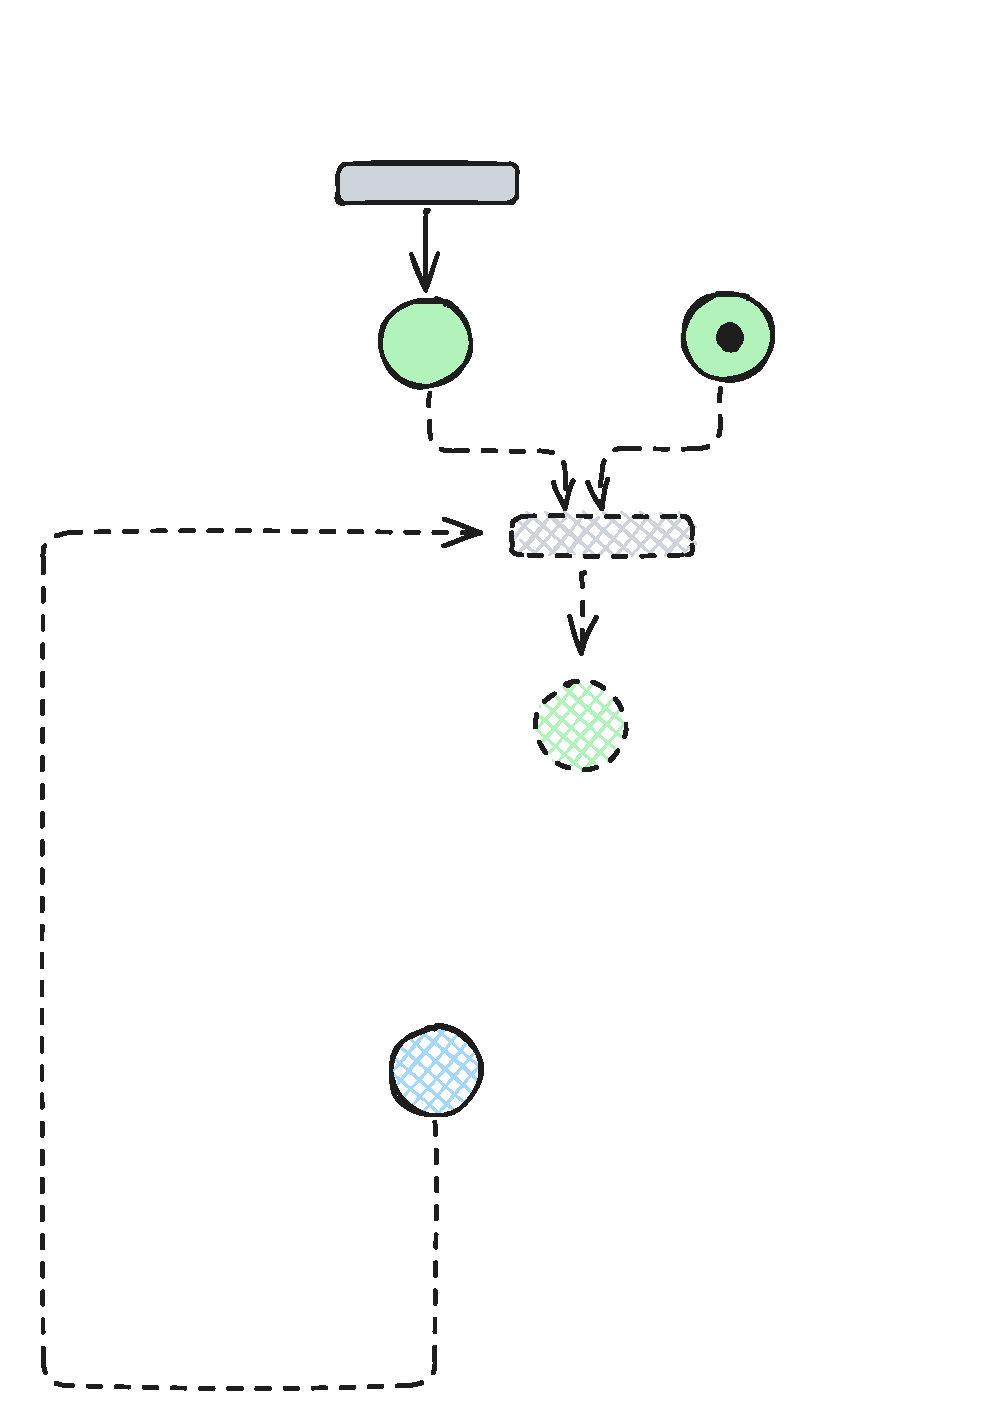
\includegraphics[width=0.23\textwidth]{plots/bidirectional_pruning_step_d_updated_2.pdf}%
	}%
}

% This forces \citet, \citep, etc. to behave like numeric \cite.
%\makeatletter
%\@ifpackageloaded{natbib}{}{%
%	\let\citet\cite
%	\let\citep\cite
%	\let\citealt\cite
%	\let\citealp\cite
%	\let\citeyear\relax
%	\let\citeauthor\relax
%}
%\makeatother

% Length-related magic, to be removed for final version
\addtolength{\oddsidemargin}{-0.2cm}
\addtolength{\evensidemargin}{-0.2cm}
\addtolength{\textwidth}{0.4cm}
\addtolength{\topmargin}{-0.1cm}
\addtolength{\textheight}{0.4cm}
\addtolength{\intextsep}{-0.4cm}
\addtolength{\belowcaptionskip}{-0.2cm}
\begin{document}

\raggedbottom


%\begin{abstract}
%	Abstract goes here
%\end{abstract}

\maketitle

\begin{abstract}
	We introduce the \toolname{} modeling language and toolchain for automatically verifying or disproving serializability of concurrent programs, i.e., whether every concurrent execution of the program is equivalent to some serial execution.
	%
	\toolname{} programs are suitably restricted to make this problem decidable, while still allowing for an unbounded number of concurrent threads of execution, each potentially running for an unbounded number of steps.
	%
	Prior work has shown theoretical decidability of this problem, but \toolname{} is the first to provide an end-to-end decision procedure and toolchain that proves serializability (generating a proof certificate) or non-serializability (generating a counterexample trace).
	%
	Our verifier operates by translating network system programs into Petri nets, and curtails the search space by employing various optimizations, such as Petri net pruning, semilinear-set compression, and Presburger-formula manipulation.
	%
	We extensively evaluate our toolchain, and demonstrate that, despite the theoretical harndess of the problem, it can successfully run on various real-world programs, including stateful firewalls, BGP routers, online shopping backends, and more.
\end{abstract}

% \keywords{programming languages, static analysis, verification}

\section{Introduction}
\label{sec:introduction}

For concurrent systems, from databases to software-defined networks (SDNs), a cornerstone correctness criterion is \emph{serializability}: every concurrent execution must produce outcomes equivalent to some serial ordering of requests. Violations of serializability can lead to subtle anomalies, such as lost updates in databases or routing cycles in SDNs.
While we can check serializability for a fixed number of requests with known execution steps by enumerating all interleavings, the problem is undecidable for general programs, requiring techniques such as runtime verification or incomplete bounded model checking \cite{WaSt06a,WaSt06b,FlFrYi08,FaMa08,SiMaWaGu11a,SiMaWaGu11b,Pa79,AlMcPe96,BiEn19}.

However, \citet{BoEmEnHa13} have shown (as a special case of bounded-barrier linearizability) that the problem is decidable for programs with bounded-size global state and bounded per-request state even for an \emph{unbounded} number of in-flight requests each performing an \emph{unbounded} number of steps. The purpose of this paper is to make this theoretical decidability result a reality by designing practical algorithms that either prove serializability (with a proof certificate) or prove non-serializability (with a counter-example trace).
% 
We illustrate the problem by example:

% examples in Listings~\ref{lst:MotivatingExample1Ser},~\ref{lst:MotivatingExample2NonSer}, and ~\ref{lst:MotivatingExample3Ser}, written in our modeling language called Ser.

\noindent
\begin{minipage}[t]{0.55\textwidth}
	\begin{minipage}[t]{\textwidth}
		\begin{lstlisting}[caption={Without yield or lock (serializable)},
			label={lst:MotivatingExample1Ser}]
  // request handler invoked by clients          
  request main: 
      X := 1 // X is global (uppercase)
      y := X // y is local (lowercase)
      X := 0
      return y 
		\end{lstlisting}
	\end{minipage}
	\vspace{1em}
	\begin{minipage}[t]{\textwidth}
		\begin{lstlisting}[caption={With yield (not serializable)},
			label={lst:MotivatingExample2NonSer}]
  request main: 
      X := 1 
      yield // let another request run
      y := X // can read 0!
      X := 0
      return y 	
		\end{lstlisting}
	\end{minipage}
\end{minipage}%
\hfill
\begin{minipage}[t]{0.35\textwidth}
	\begin{lstlisting}[caption={With yield and lock (serializable)},
		label={lst:MotivatingExample3Ser}]
  request main: 
      // lock
      while (L == 1): 
          yield
      L := 1 

      X := 1
      yield
      y := X 
      X := 0

      // unlock    
      L := 0
      return y 
	\end{lstlisting}
\end{minipage}

These examples are written in our modeling language called Ser.
A Ser program has a set of named \textbf{request handlers} (one handler \texttt{main} in the examples) that are arbitrarily invoked concurrently by the external environment.
Each incoming request processes its request handler's body until it returns a value as its \textbf{response}. Concurrency is managed by the \textbf{yield} statement, which pauses the current request and gives other requests a chance to run. Ser programs have uppercase \textbf{global shared variables} (\texttt{X} in the examples) and lowercase \textbf{request-local variables} (\texttt{y} in the examples).



%
The first program (Listing~\ref{lst:MotivatingExample1Ser}) is clearly serializable because there are no yields, and hence, no interleavings: each \texttt{main} request returns 1.
In the second program (Listing~\ref{lst:MotivatingExample2NonSer}), the yield allows interleavings and is \emph{not} serializable; consider two concurrent requests to \texttt{main}:
\begin{enumerate}
\item Request A executes \texttt{X := 1} then yields to Request B
\item Request B executes \texttt{X := 1}, yields to itself, reads \texttt{X} (getting 1), sets \texttt{X := 0}, and returns 1
\item Request A resumes, reads \texttt{X} (now 0), and returns 0
\end{enumerate}
This produces the multiset \{(\texttt{main}, 0), (\texttt{main}, 1)\} of (request, response) pairs, which is impossible in any serial execution (where all \texttt{main} requests return 1 and never 0).
Of course, having yields does not guarantee that an execution is necessarily not serializable, as observed in the third snippet (Listing~\ref{lst:MotivatingExample3Ser}). This program uses an additional lock variable ``L'', which guarantees that even if an interleaving occurs, the program is semantically equivalent to the first one.
%
These examples demonstrate that reasoning about serializability can be complex even for very simple programs with few requests running concurrently.
\vspace{-.5em}
\paragraph{Problem Definition.}
Formally, we define the \textbf{observable execution} of a Ser program as a multiset of (request, response) pairs. The \textbf{observable behavior} of a Ser program is the set of all possible observable executions that can occur such that the requests are executed concurrently to obtain their paired responses.
A program is \textbf{serializable} if every observable behavior is achievable serially (without interleavings). That is, a Ser program is serializable if its semantics does not change when all yield statements are removed.
%
\emph{The goal of this paper is to design and develop the Ser language and decision procedure for this problem.} In particular, Ser can prove serializability \textbf{automatically} without requiring any manual proof by the user.
\vspace{-.5em}
\paragraph{Challenges.}
To our knowledge, no prior implementation exists that can automatically generate proof certificates for this class of concurrent systems.
Why not?
Our decision procedure builds on Bouajjani et al.'s reduction from serializability to Petri net reachability~\cite{BoEmEnHa13}. However, since Petri net reachability is Ackermann-complete~\cite{CzWo22}, a naive implementation would fail on all but the simplest programs. 
\vspace{-.5em}
\paragraph{Our Approach.}
To address this, we first introduce the abstraction of \textit{network systems} (NS) --- abstract concurrent programs where users send \textit{requests} that manipulate local and shared state before returning \textit{responses}. Ser programs are compiled into NS, on which our decision procedure operates via reduction to Petri net and semilinear set analysis.

As a backend solver, we use SMPT~\cite{AmDa23}, which is a state-of-the-art tool for Petri net reachability.
We note that while our approach is sound (never incorrectly claims serializability), the underlying SMPT Petri Net tool may time out on complex instances, limiting completeness in practice (which is unavoidable for any Petri Net tool, given the Ackermann-completeness of the problem).

We developed several techniques to make the approach practical, including Petri Net pruning, semilinear set compression, and additional manipulations with Presburger formulas.
These optimizations reduce the search space by orders of magnitude, enabling us to successfully verify the serializability of non-trivial programs.

We evaluated our approach on programs with features such as loops, branching, locks, and nondeterminism. Our benchmarks include SDN-inspired examples such as stateful firewalls, BGP routing, and online shopping systems.

To our knowledge, this leads to the first \emph{implemented} decision procedure that: (i) automatically \textit{proves} serializability for unbounded executions; (ii) generates \textit{proof certificates}; and (iii) handles non-trivial programs.


\paragraph{Contributions.}
After a tour of examples in \Cref{sec:tour}, we present the following contributions:
\begin{itemize}
    \item \Cref{sec:problem-definition} introduces the notion of a Network System (NS), a concurrent program abstraction that captures the essence of concurrent systems.
    \item \Cref{sec:formal-results} presents decidability results (a theorem on serializability; two on equivalence), presents the core decision procedure with proof certificates, and presents techniques for semilinear set reductions and Petri-net reductions.
    \item \Cref{sec:implementation} presents the implementation of the Ser toolchain.
    \item \Cref{sec:evaluation} presents case studies on modeling in Ser examples from domains such as SDNs and databases, and presents our extensive evaluation of the toolchain.
\end{itemize}


Finally, we discuss related work in \Cref{sec:related-work} and conclude in \Cref{sec:discussion}.
Our tool, benchmarks, and experiments are available as an anonymous artifact~\cite{ArtifactRepository} and will be permanently hosted with the paper’s final version. There is also a technical appendix accompanying this paper.
\section{Problem Definition}
\label{sec:problemDefinition}

\newcommand{\grammartag}[1]{\qquad\qquad\emph{(#1)}}
\begin{figure}[t]
    \begin{align*}
    \mathbf{Expression}\quad e ::= &&& \\
       | & \quad 0 \mid 1 \mid 2 \mid \ldots                                && \grammartag{Numeric constants} \\
       | & \quad \nondet                                 && \grammartag{Nondeterministic value: 0 or 1}\\
       | & \quad x := e                            && \grammartag{Write to local packet field} \\
       | & \quad x                                 && \grammartag{Read from local packet field} \\
       | & \quad X := e                            && \grammartag{Write to global switch variable} \\
       | & \quad X                                 && \grammartag{Read from global switch variable} \\
       | & \quad e_1 == e_2                        && \grammartag{Equality test} \\
       | & \quad e_1 ; e_2                         && \grammartag{Sequencing} \\
       | & \quad \ifkw(e_1)\{\ e_2\ \}\elsekw\{\ e_3\ \} && \grammartag{Conditional} \\
       | & \quad \whilekw(e_1)\{\ e_2\ \}              && \grammartag{While loop} \\
       | & \quad \yieldkw                      && \grammartag{Yields to scheduler}\\[1em]
    \mathbf{Program}\quad p ::=
        & \quad \requestkw\ name_1\ \{\ e_1\ \}&&\grammartag{Set of request handlers}\\[-0.5em]
        & \quad \qquad \vdots &&\\
        & \quad \requestkw\ name_n\ \{\ e_n\ \}\ 
    \end{align*}
    \caption{Syntax of expressians and programs}
    \label{fig:syntax}
\end{figure}
    
A Network System $\mathcal{N}$ is a tuple $(G, L, \mathit{Req}, \mathit{Res}, g_0, \delta, \mathit{req}, \mathit{resp})$ where:
\begin{itemize}
\item $G$ is a set of global states representing switch state
\item $L$ is a set of local states representing packet contents
\item $\mathit{Req}$ is a set of request events
\item $\mathit{Res}$ is a set of response events
\item $g_0 \in G$ is the initial global state
\item $\mathit{req} \subseteq \mathit{Req} \times L$ is a request transition relation, which describes which requests turn into which packets
\item $\mathit{resp} \subseteq L \times \mathit{Res}$ is a response transition relation, which describes which packets turn into which responses
\item $\delta \subseteq (G \times L) \times (G \times L)$ is a transition relation for packet processing, which describes an atomic step of packet processing that may change the global state.
\end{itemize}

\begin{figure}[t]
    \centering
    \renewcommand{\arraystretch}{1.6}
    \[
    \begin{array}{c}
    \textbf{States and Transitions:}
    \\
    \quad
    \text{A (global) \emph{network state} is a triple }(g,\mathcal{P},M)\text{ where:}
    \\
    \quad
    g \in G \text{ is the current global switch state,}
    \\
    \quad
    \mathcal{P} \in \text{Multiset}(L \times \mathit{Req}) \text{ is a multiset of in-flight packets,}
    \\
    \quad
    M \in \text{Multiset}(\mathit{Req} \times \mathit{Res}) \text{ is a multiset of request--response pairs already completed.}
    \end{array}
    \]

    \[
    \begin{array}{c}
    \textbf{Initial state:}
    \\
    \quad (g_0,\,\varnothing,\,\varnothing)
    \end{array}
    \]

    \[
    \begin{array}{c}
    \textbf{Transition rules:}
    \\[1em]
    \text{(New Request)}\quad\infer{
    (r,\ell)\,\in\,\mathit{req}
    }
    {(g,\;\mathcal{P},\;M) \;\longrightarrow\; (g,\;\mathcal{P} \uplus \{(\ell,r)\},\;M)}
    \\[2em]
    \text{(Packet Step)}\quad\infer{
    ((g,\ell),\,(g',\ell')) \,\in\, \delta
    }
    {(g,\;\mathcal{P} \uplus \{(\ell,r)\},\;M) \;\longrightarrow\; (g',\;\mathcal{P} \uplus \{(\ell',r)\},\;M)}
    \\[2em]
    \text{(Response)}\quad\infer{
    (\ell,s)\,\in\,\mathit{resp}
    }
    {(g,\;\mathcal{P} \uplus \{(\ell,r)\},\;M) \;\longrightarrow\; (g,\;\mathcal{P},\;M \uplus \{(r,s)\})}
    \end{array}
    \]

    \[
    \begin{array}{c}
    \textbf{Complete runs:}
    \\
    \quad (g_0,\,\varnothing,\,\varnothing) \;\longrightarrow\; (g_1,\,\mathcal{P}_1,\,M_1) \;\longrightarrow\; \cdots \;\longrightarrow\; (g_n,\,\mathcal{P}_{n-1},\,M_{n-1}) \;\longrightarrow\; (g_n,\,\varnothing,\,M_n)
    \\[1em]
    \textbf{Interleaved run: } \text{the } \mathcal{P}_i \text{ can have more than one packet, and } \mathcal{P}_n = \varnothing \\
    \textbf{Serial run: } \text{ each } \mathcal{P}_i \text{ has at most one packet, and } \mathcal{P}_n = \varnothing\\
    \text{Int}(\mathcal{N}) = \{ M \in \text{Multiset}(\mathit{Req} \times \mathit{Res}) \mid \exists \text{ interleaved run } (g_0,\,\varnothing,\,\varnothing) \;\longrightarrow^*\; (g_n,\,\varnothing,\,M) \}\\
    \text{Ser}(\mathcal{N}) = \{ M \in \text{Multiset}(\mathit{Req} \times \mathit{Res}) \mid \exists \text{ serial run } (g_0,\,\varnothing,\,\varnothing) \;\longrightarrow^*\; (g_n,\,\varnothing,\,M) \}\\
    \end{array}
    \]

    \caption{State-transition rules for executions of
    \(\mathcal{N} = (G, L, \mathit{Req}, \mathit{Res}, g_0, \delta, \mathit{req}, \mathit{resp})\).
    A transition \(\longrightarrow\) modifies the triple \((g,\mathcal{P},M)\) by either (1) introducing a new request, (2) processing a packet step via \(\delta\), or (3) consuming a packet to produce its response.  When no more steps are possible, the result set \(M\) is the final multiset of request--response pairs that arose during the run.
    Runs are called \emph{serial} if there is at most one packet in flight at any time, whereas \emph{interleaved} runs may have multiple packets in flight at once.}
    \label{fig:network-transitions}
\end{figure}

\begin{definition}[Interleaved executions \(\mathrm{Int}(\mathcal{N})\)]
    Let \(\mathcal{N} = (G, L, \mathit{Req}, \mathit{Res}, g_0, \delta, \mathit{req}, \mathit{resp})\).
    An \emph{interleaved execution} begins in global state \(g = g_0\) with no packets in flight.
    At any point, one may:
    \begin{itemize}
        \item introduce a new request \(r \in \mathit{Req}\), producing an in-flight packet \(\ell \in L\) if \((r,\ell) \in \mathit{req}\);
        \item take an in-flight packet \(\ell\) and transition \(\ell \mapsto \ell'\) and \(g \mapsto g'\) if \(((g,\ell),(g',\ell'))\in\delta\);
        \item consume an in-flight packet \(\ell\) to produce a response \(s\) if \((\ell,s)\in \mathit{resp}\).
    \end{itemize}
    Each request \(r\) must eventually yield exactly one corresponding response \(s\) in a valid execution.
    The set of all finite multisets of \((r,s)\) pairs realizable by such interleavings is:
    \[
        \mathrm{Int}(\mathcal{N})
        \;=\;
        \bigl\{
        M \;\in\; \text{Multiset}(\mathit{Req}\times \mathit{Res})
        \;\mid\;
        M \text{ is realized by some interleaved run of }\mathcal{N}
        \bigr\}.
    \]
\end{definition}

\begin{definition}[Serial executions \(\mathrm{Ser}(\mathcal{N})\)]
In a \emph{serial} execution, requests are processed one at a time:
\begin{enumerate}
    \item Start in \(\,g_0\).
    \item Take a single request \(r\in \mathit{Req}\), convert it to a packet, process that packet until a response \(s\in \mathit{Res}\) is produced.
    \item Update the global state accordingly and repeat with the next request.
\end{enumerate}
No two requests overlap in processing.
The set of all finite multisets of \((r,s)\) pairs realizable by such one-at-a-time runs is:
\[
    \mathrm{Ser}(\mathcal{N})
    \;=\;
    \bigl\{
    M \;\in\; \text{Multiset}(\mathit{Req}\times \mathit{Res})
    \;\mid\;
    M \text{ is realized by some serial run of }\mathcal{N}
    \bigr\}.
\]
\end{definition}

\begin{theorem}[Serializability]
\label{thm:int-eq-ser}
Whether
\(
    \mathrm{Int}(\mathcal{N}) \;=\; \mathrm{Ser}(\mathcal{N})
\)
holds is decidable.
\end{theorem}

\begin{theorem}[Serial Equivalence]
\label{thm:ser-eq-ser}
Whether
\(
    \mathrm{Ser}(\mathcal{N}) \;=\; \mathrm{Ser}(\mathcal{N})
\)
holds is decidable.
\end{theorem}

\begin{theorem}[Interleaved Equivalence]
\label{thm:int-eq-int}
Whether
\(
    \mathrm{Int}(\mathcal{N}) \;=\; \mathrm{Int}(\mathcal{N})
\)
holds is undecidable.
\end{theorem}
\section{Formal results}
\label{sec:formal-results}

%\begin{itemize}
%	\item Results that we rely on (petri nets, semilinear sets)
%	\item The base algorithm described in math (without any optimizations)
%	\item Time complexity
%	\item proof for correctness of bidirectional pruning
%	\item mathematical description of optimizations
%\end{itemize}




\subsection{The Algorithm (without Optimizations)}

Given a network system \(\mathcal S\) with global states \(G\), our algorithm proceeds as follows:  

\begin{enumerate}
	\item  \textbf{Serializability automaton.} 
	We define an NFA 
	\(
	\mathcal A_{\mathrm{ser}}(\mathcal S)=(Q,\Sigma,\delta,q_0,F)
	\), with
	\( Q=G,\;F=G,\;q_0=g_0,
	\)
	over an alphabet
	\(
	\Sigma=\{({\color{ForestGreen}\blacklozenge_{\mathit{req}}}/{\color{red}\blacklozenge_{\mathit{resp}}})
	\mid {\color{ForestGreen}\blacklozenge_{\mathit{req}}}\in\mathit{REQ},\;
	{\color{red}\blacklozenge_{\mathit{resp}}}\in\mathit{RESP}\}.
	\)
%	
%	\todo{old}
%	We define an NFA
%	\[
%	\mathcal A_{\mathrm{ser}}(\mathcal S)
%	= \bigl(Q,\Sigma,\delta,q_0,F\bigr),
%	\quad
%	Q = G,\quad F = G \;\;(\text{global states}),\quad
%	q_0 = g_0 \;\;(\text{initial state}),
%	\]
%	\[
%	\Sigma
%	= \Bigl\{
%	({\color{ForestGreen}\blacklozenge_{\mathit{req}}}\,/\,%
%	{\color{red}\blacklozenge_{\mathit{resp}}})
%	\;\Big|\;
%	{\color{ForestGreen}\blacklozenge_{\mathit{req}}}\in\mathit{REQ},\;
%	{\color{red}\blacklozenge_{\mathit{resp}}}\in\mathit{RESP}
%	\Bigr\}.
%	\]
%
Finally, we define:
\(
\delta \subseteq Q \times \Sigma \times Q,
\qquad q \xrightarrow{{\color{ForestGreen}\blacklozenge_{\mathit{req}}}/{\color{red}\blacklozenge_{\mathit{resp}}}} q'
\),
%old
%\(
%\delta \;\subseteq\; Q \times \Sigma_{	{\color{ForestGreen}\blacklozenge_{\mathit{req}}}\,/\,%
%	{\color{red}\blacklozenge_{\mathit{resp}}}} \times Q,
%\quad
%\bigl(q \xrightarrow{%
%	{\color{ForestGreen}\blacklozenge_{\mathit{req}}}\,/\,%
%	{\color{red}\blacklozenge_{\mathit{resp}}}%
%} q'\bigr),
%\)
%
%\;\Longleftrightarrow\;
%\begin{array}{l}
iff $\mathcal S$ is in global state $q$ and issues a request
$	{\color{ForestGreen}\blacklozenge_{\mathit{req}}}$, then upon completion it receives response $	{\color{red}\blacklozenge_{\mathit{resp}}}$
	and transitions to global state  $q'$,
%\end{array}
%\]
%
%
%
%
%
%
%\begin{array}{l}
%	\mathcal S \text{ at global state } q
%	\;\text{issues}\;
%	{\color{ForestGreen}\blacklozenge_{\mathit{req}}},\\[0.5ex]
%	\text{after full completion of the request, it receives}\;
%	{\color{red}\blacklozenge_{\mathit{resp}}},\\[0.5ex]
%	\text{arriving at global state } q'
%\end{array}
%\]
%
%	
i.e., each transition is a request/response pair.  Its language
	\(L(\mathcal A_{\mathrm{ser}})\subseteq\Sigma^*\) is exactly the set of serial
	request/response traces, and we define the semilinear set of serial executions, each such execution giving rise to a multiset of request/response pairs:
	\(
	\mathsf{Ser}(\mathcal S)
	\;=\;
	\mathsf{Parikh}\bigl(L(\mathcal A_{\mathrm{ser}})\bigr)
	\;\subseteq\;\mathbb N^{\Sigma}.
	\)
%	Finally,
%	\(
%	q_0 = g_0
%	\quad\text{(the initial global state of the NS)}
%	\).
	
	
%	\smallskip
\begin{tcolorbox}[colback=black!5!white, colframe=black, boxrule=1pt]
	\textbf{Example.} In the case of the toy (non-serializable) program presented in Listing~\ref{lst:MotivatingExample2NonSer}, the NS depicted in Fig.~\ref{fig:code2ExampleNS} allows us to also extract the NFA encoding all serial executions. The states encode the global variable values, and the edges encode request/response pairs for all serial executions. As can be seen in Fig.~\ref{fig:code2ExampleNFA}, serial executions can produce only request/response pairs of the type ({\color{ForestGreen}$\blacklozenge_\text{main}$/{\color{red}$\blacklozenge_1$}}). Furthermore, the only global state reachable in serial executions, when a request enters and exits the system, is [X=0]. 
	%
	Intuitively, this corresponds to [X=0] being the initial global state, as well as the system's global state after every single packet exits the network in a serializable execution.
	\end{tcolorbox}
	%
	\begin{figure}[!htbp]
		\centering
		% 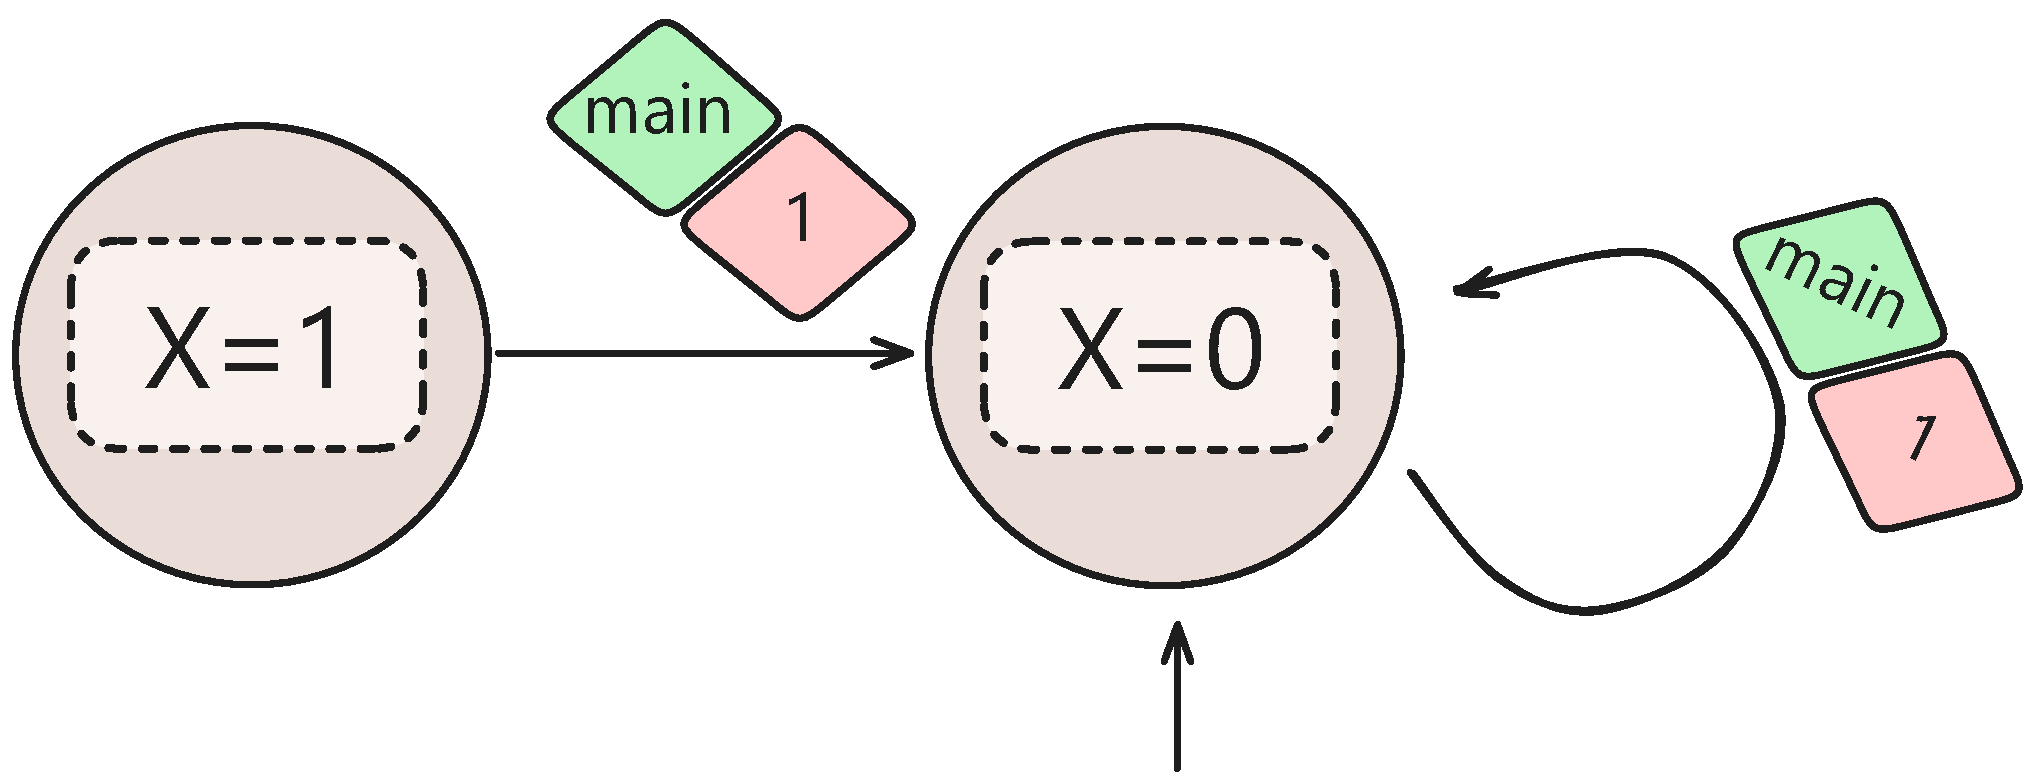
\includegraphics[width=0.48\textwidth,trim=0 0 0 0,clip]{plots/code_2_NFA_v3.pdf}
		
		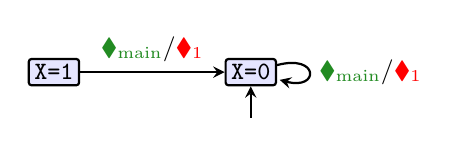
\begin{tikzpicture}[
			->,>=stealth,
			thick,
			node distance=2.5cm,
			state/.style={
				draw=black,
				line width=0.8pt,
				fill=blue!10,
				rectangle,
				rounded corners=1pt,
				inner sep=2pt,
				font=\small
			},
			every node/.style={font=\small}
			]
			% States using the same notation as section 3
			\node[state] (X1) {\texttt{X=1}};
			\node[state, right of=X1] (X0) {\texttt{X=0}};
			
			% Initial state arrow
			\draw[->] ([yshift=-0.4cm]X0.south) -- (X0.south);
			
			% Transitions with proper colored notation from the paper
			\draw[->] (X1) -- node[above] {${\color{ForestGreen}\blacklozenge_{\mathrm{main}}}/{\color{red}\blacklozenge_1}$} (X0);
			\draw[->] (X0) edge[loop right] node[right] {${\color{ForestGreen}\blacklozenge_{\mathrm{main}}}/{\color{red}\blacklozenge_1}$} (X0);
		\end{tikzpicture}
		
		\caption{Serial NFA of Listing~\ref{lst:MotivatingExample2NonSer}.}
		\label{fig:code2ExampleNFA}
	\end{figure}
	
	

	
%	\begin{wrapfigure}{r}{0.50\textwidth}  % “r” = right, width = 0.5\textwidth
%		\centering
%		% 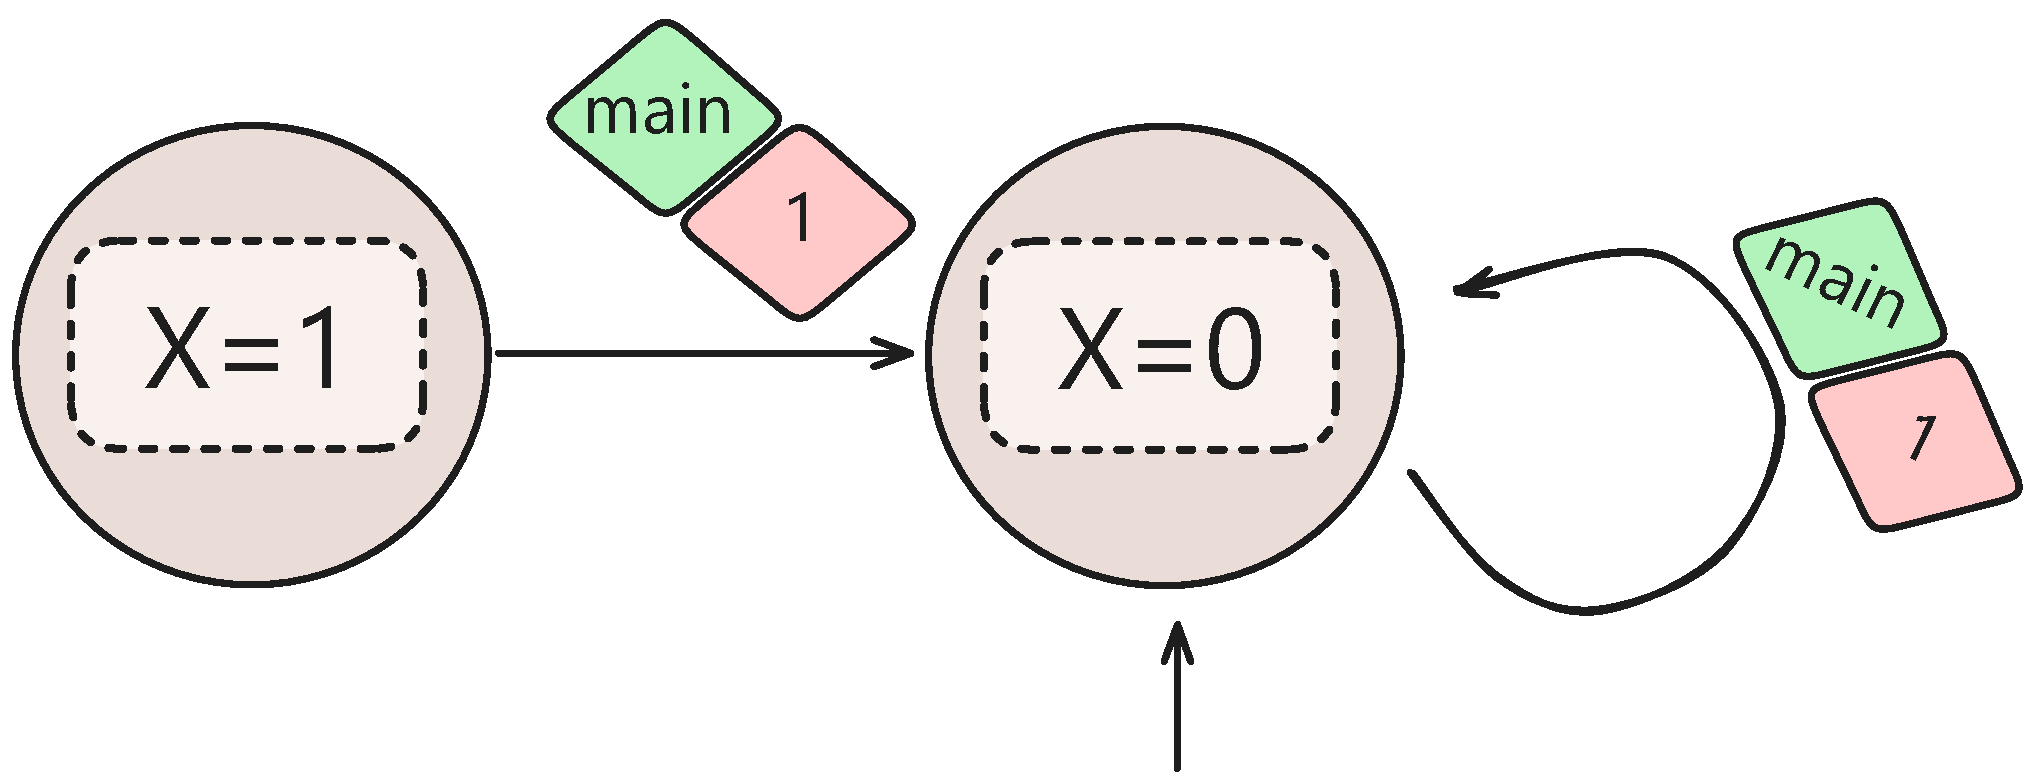
\includegraphics[width=0.48\textwidth,trim=0 0 0 0,clip]{plots/code_2_NFA_v3.pdf}
%		
%		\begin{tikzpicture}[
%			->,>=stealth,
%			thick,
%			node distance=2.5cm,
%			state/.style={
%				draw=black,
%				line width=0.8pt,
%				fill=blue!10,
%				rectangle,
%				rounded corners=1pt,
%				inner sep=2pt,
%				font=\small
%			},
%			every node/.style={font=\small}
%			]
%			% States using the same notation as section 3
%			\node[state] (X1) {\texttt{X=1}};
%			\node[state, right of=X1] (X0) {\texttt{X=0}};
%			
%			% Initial state arrow
%			\draw[->] ([yshift=-0.4cm]X0.south) -- (X0.south);
%			
%			% Transitions with proper colored notation from the paper
%			\draw[->] (X1) -- node[above] {${\color{ForestGreen}\blacklozenge_{\mathrm{main}}}/{\color{red}\blacklozenge_1}$} (X0);
%			\draw[->] (X0) edge[loop right] node[right] {${\color{ForestGreen}\blacklozenge_{\mathrm{main}}}/{\color{red}\blacklozenge_1}$} (X0);
%		\end{tikzpicture}
%		
%		\caption{Serial NFA of Listing~\ref{lst:MotivatingExample2NonSer}.}
%		\label{fig:code2ExampleNFA}
%	\end{wrapfigure}
	%
	%
	%Intuitively, this corresponds to the Listing~\ref{lst:MotivatingExample2NonSer} program updating [X:=1] as an intermediate assignment before yielding.
	
	
	
	\item 
	\textbf{Interleaving Petri Net.}
%	
Next, we translate the NS into a Petri Net \(N_{\mathrm{int}}(\mathcal S)\). The \textit{non-sink places} of the PN represent either (i) global state assignments; and (ii) local states of an in-flight packet. The \textit{sink} places represent request/response pairs of terminating packets.
%
We define the \textit{transitions} between states to correspond to the \(\delta\),\(req\), and \(resp\) mappings of the NS, and with the transitions of the request being able to fire without any input tokens (in order to correspond to initializing arbitrary external requests).
%
Finally, we define the initial marking \(M_0\) to correspond to a single token in the initial global state \(g_0\).
%
This construction (which is fully formalized in Appendix~\ref{appendix:NS-to-PN-formulation}) guarantees that the multiset of all reachable markings \(M\) (with \(M_0 \xrightarrow{}^{*} M\)) projected to the sink places, corresponds to the multiset of all  (${{\color{ForestGreen}\blacklozenge_{\mathit{req}}}/{\color{red}\blacklozenge_{\mathit{resp}}}}$) pairs of the NS, attained by any interleaving, i.e., \(\mathsf{Int}(\mathcal S)\).



\begin{tcolorbox}[colback=black!5!white, colframe=black, boxrule=1pt]
	\textbf{Example.}
%	\textit{Notation.}
In our running example, the NS gives rise to the PN in Fig.~\ref{fig:code2ExamplePN}, encoding all possible interleavings. The places \textcolor{blue}{ $P_2$} and \textcolor{blue}{$P_3$} represent the global states \textcolor{blue}{[X=1]} and \textcolor{blue}{[X=0]}, respectively, while the places $P_1$, $P_4$, $P_5$, and $P_6$ capture the local states of in-flight requests—that is, the remaining program code together with the assignments to each request’s local variables. Similarly, places \textcolor{red}{$P_7$} and \textcolor{red}{$P_8$} correspond to {\color{red}$\blacklozenge_1$} and {\color{red}$\blacklozenge_0$}, respectively, encoding terminated responses. Each token either models an active request, a completed request/response pair, or --- when residing in a global-state place --- the current global state. Finally, transitions implement the network system’s mappings ($\delta/req/resp$): they advance the program by one step, spawn a new request (e.g., transition $t_1$, producing {\color{ForestGreen}$\blacklozenge_{\mathrm{main}}$}), or return a response (e.g., transitions $t_6$ and $t_7$).
\end{tcolorbox}

%Finally, the NS gives rise to the PN in Fig.~\ref{fig:code2ExamplePN}, encoding all possible interleavings.
%%
%The places represent either the global state
%(e.g., places \textcolor{blue}{$P_2$} and \textcolor{blue}{$P_3$} correspond to the global states \textcolor{blue}{[X=1]} and \textcolor{blue}{[X=0]}), while others ($P_1,P_4,P_5,P_6$) correspond to the local state of an in-flight request, i.e., combinations of ``remaining'' programs  assignments to local variables of in-flight requests.
%%
%Furthermore, some requests correspond to responses, e.g., places \textcolor{red}{$P_7$} and \textcolor{red}{$P_8$} corresponds to {\color{red}$\blacklozenge_1$} and {\color{red}$\blacklozenge_0$}.
%%
%Each token corresponds either to a single in-flight request, a single terminated pair of request/response, or (in the case of the global-variable-encoding places), to the current global state.
%%
%Finally, transitions represent the network system's $\delta$ mapping --- encoding either a ``step'' of our program, or spawning a request ($t_1$, which  corresponds to spawning {\color{ForestGreen}$\blacklozenge_\text{main}$}), or returning a response (e.g. transitions $t_6,t_7$).
%


\begin{figure}[!htbp]
	\centering
	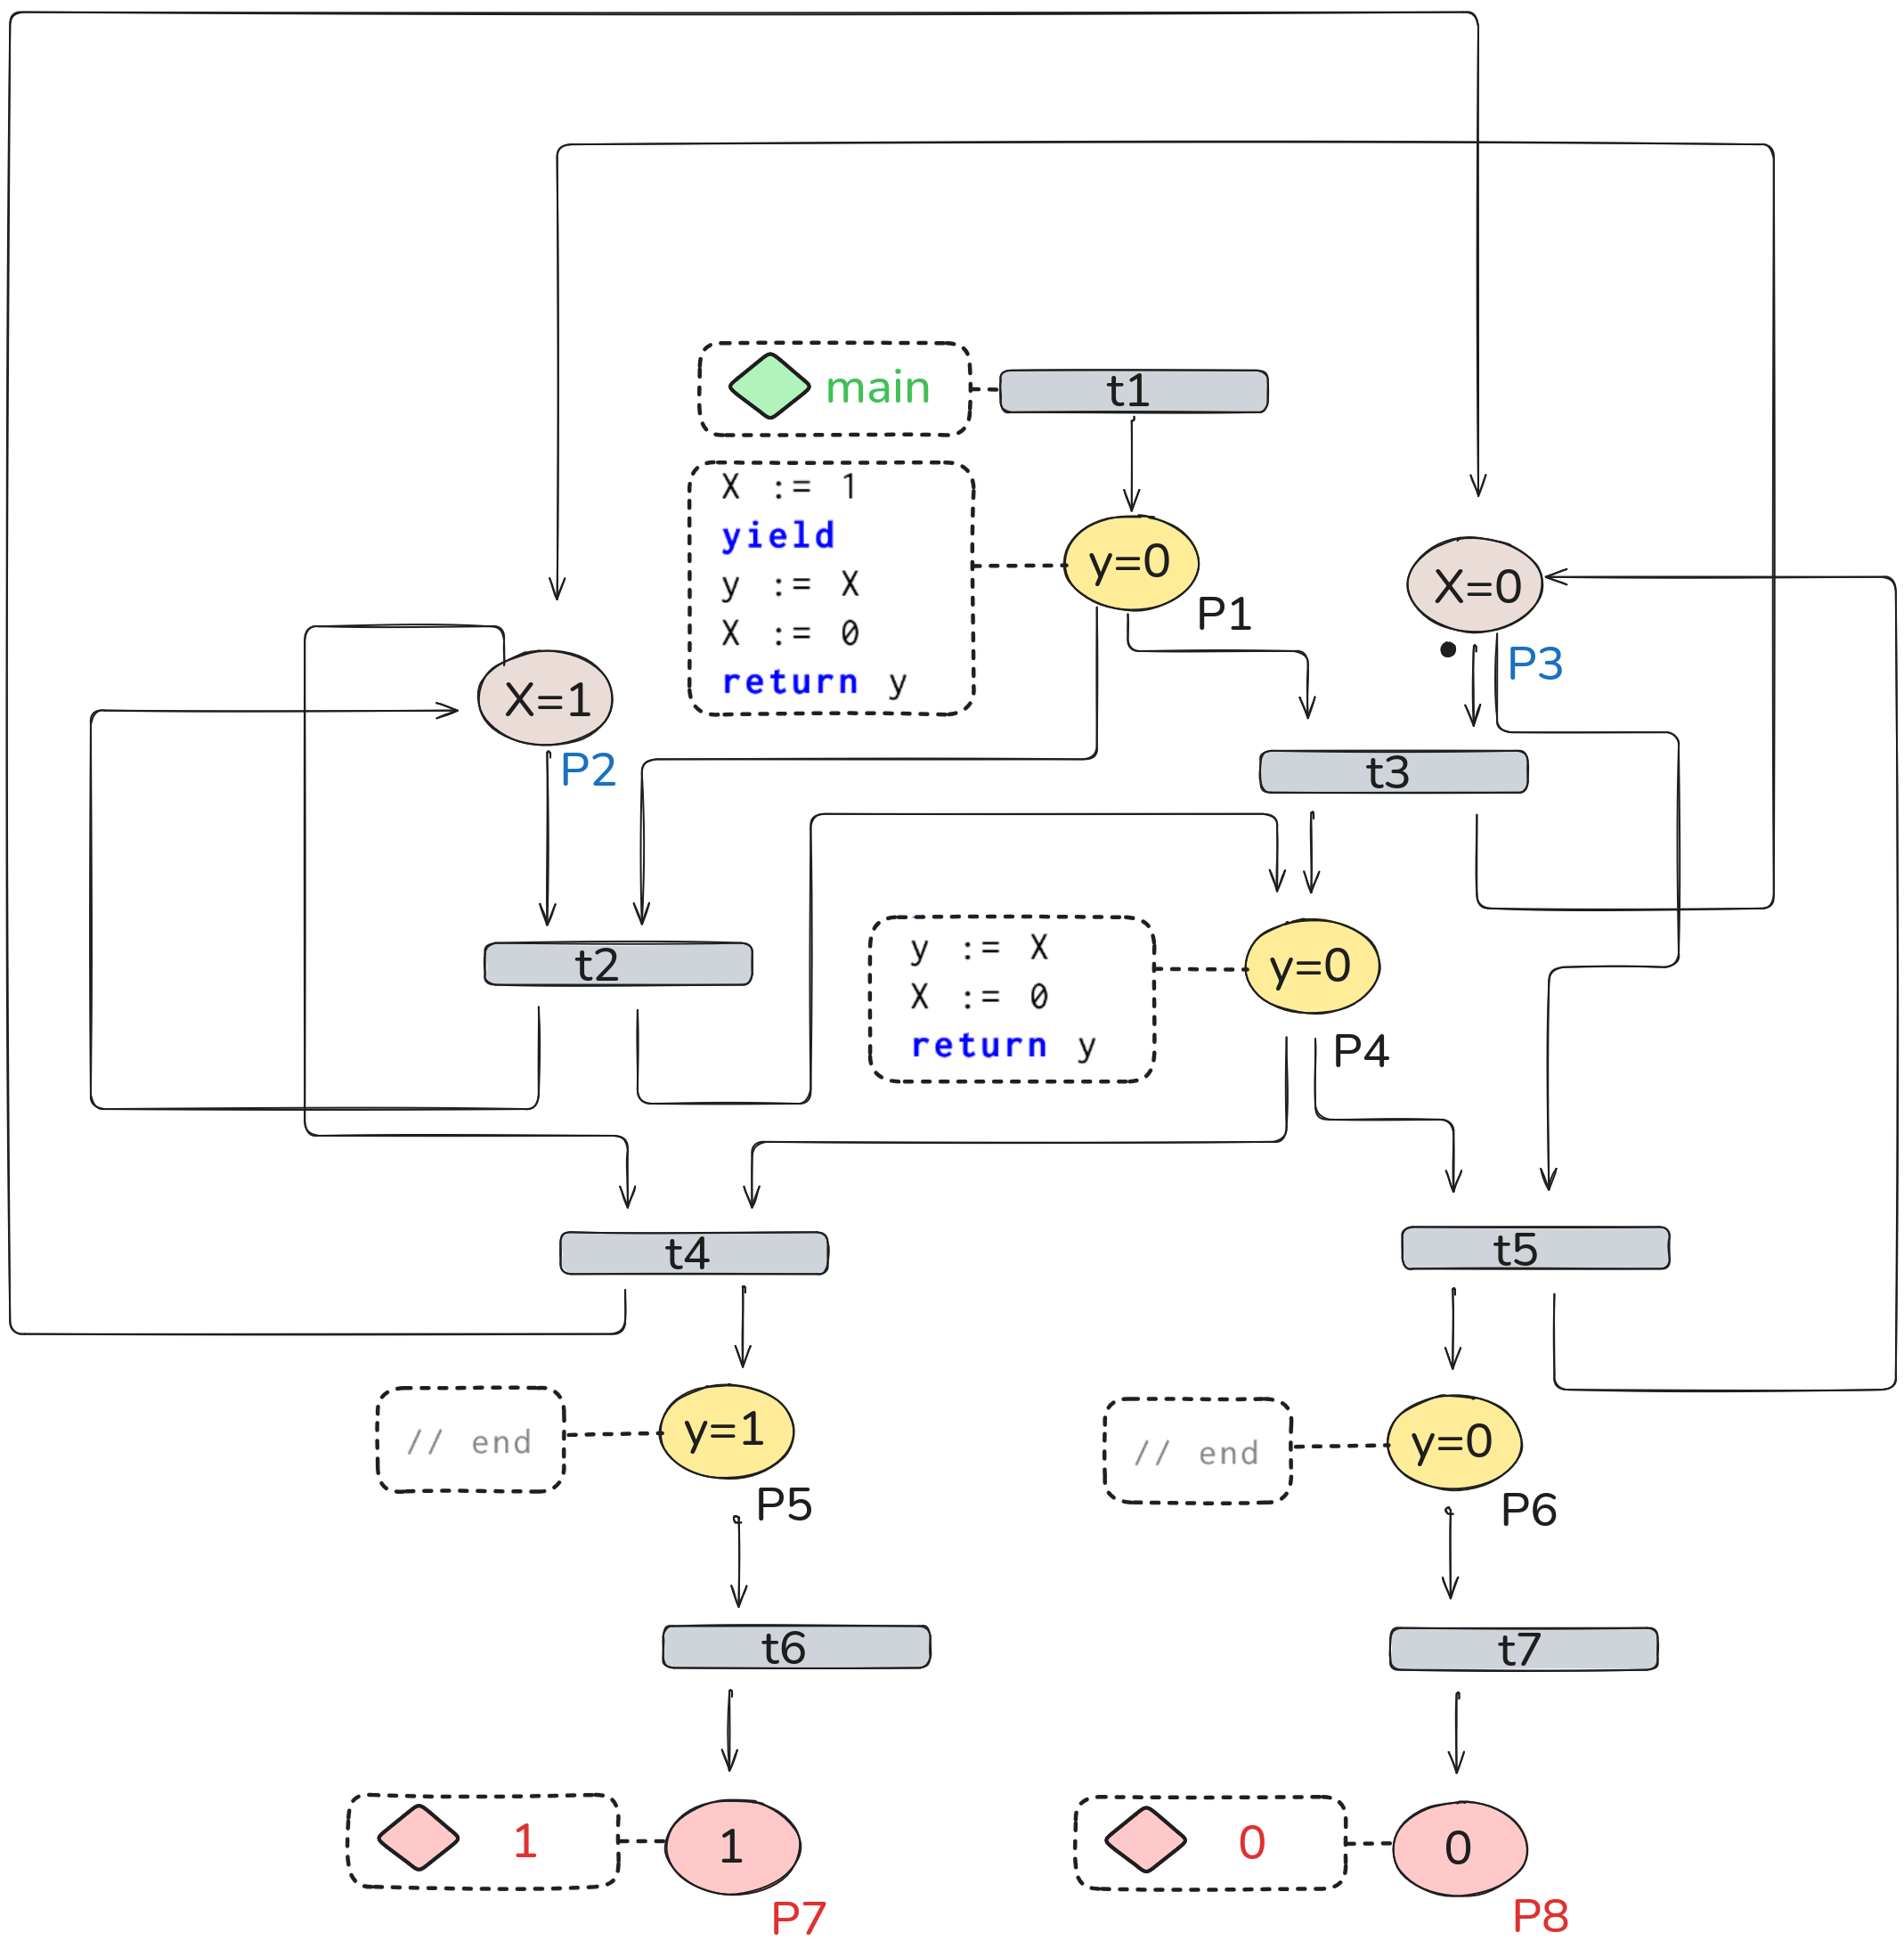
\includegraphics[width=0.7\textwidth]{plots/code_2_PN_with_annotation.png}
	\caption{The PN encoding interleaving executions of the program in Listing~\ref{lst:MotivatingExample2NonSer}.}
	\label{fig:code2ExamplePN}
\end{figure}



	
	
	\item \textbf{Non-serializable set.}  
	Let
	\(\;\mathsf{NonSer}(\mathcal S)=\mathbb N^{|\Sigma|}\setminus \mathsf{Ser}(\mathcal S)\), i.e., all (${{\color{ForestGreen}\blacklozenge_{\mathit{req}}}/{\color{red}\blacklozenge_{\mathit{resp}}}}$) pairs that \textit{cannot} be attained via a serializable execution.
	
	\begin{tcolorbox}[colback=black!5!white, colframe=black, boxrule=1pt]
	\textbf{Example.}
	Regarding the aforementioned program, we automatically generate the following reachability query\footnote{If not for the equality constraints, the problem would have been considered a \textit{coverability} query, which is easier~\cite{Ra78}.} for the Petri net in Figure~\ref{fig:code2ExamplePN}: we encode the target semilinear set by imposing the following constraints on the token distribution:
	%
	%Regarding the aforementioned program, we automatically generate the following reachability query~\footnote{If not the equality constraints, the problem would have been considered a \textit{coverability} query which is easier~\cite{Ra78}.} for the Petri net in Figure~\ref{fig:code2ExamplePN} we encode a target semilinear set with the following constraints on the token distribution:
	%
	\[
	P_1 = 0 \wedge 
	\textcolor{blue}{P_2} \ge 0 \wedge \textcolor{blue}{P_3} \ge 0  \wedge P_4 = 0
	\wedge P_5 = 0 \wedge P_6 = 0 \wedge \textcolor{red}{P_7} \ge 0 \wedge \textcolor{red}{P_8} \ge 1.
	\]
	
	This set encodes all reachable markings with no tokens on $P_1,P_4,P_5,P_6$, at least one token on $\textcolor{red}{P_8}$, and arbitrary tokens on $\textcolor{blue}{P_2},\textcolor{blue}{P_3},\textcolor{red}{P_7}$. 
	\end{tcolorbox} 
	
	
%	\item \textbf{Reachability encoding.}  
	
	
	\item \textbf{Decision \& Validation.}  
	Ask whether there exists a marking \(M\) of \(N_{\mathrm{int}}(\mathcal S)\) such that
	\[
	M_0 \xrightarrow{}^{*} M
	\quad\wedge\quad
	\pi(M)\in \mathsf{NonSer}(\mathcal S).
	\]
	
	\begin{itemize}
		\item [\sat]: yields a counterexample interleaving \(M\) with
		\(\pi(M)\notin \mathsf{Ser}(\mathcal S)\), which is automatically embedded into the NS semantics.
%		We validate a reachable trace and embed it into the NS semantics, yielding a valid interleaving that produces request/response pairs unattainable under any serial execution.
		
		\item [\unsat]: yields an inductive invariant of
		\(N_{\mathrm{int}}\), which back-translates to a proof of
		serializability 
		for \(\mathcal S\),
		%
		validated by synthesizing an inductive invariant over the interleaving PN, thereby proving that the corresponding semilinear set cannot be realized by any interleaving (see Appendix~\ref{appendix:ns-serializable}).
	\end{itemize}

\begin{tcolorbox}[colback=black!5!white, colframe=black, boxrule=1pt]
	\textbf{Example.}
	This target semilinear set of markings is, in fact non-empty. For example, it includes the following reachable marking:
	
	\[
	M^* = \{\textcolor{blue}{P_3}(1),\;\textcolor{red}{P_7}(1),\;\textcolor{red}{P_8}(1)\}
	\]
	
	Table~\ref{tab:PetriNetFiringCounterexample} (in Appendix~\ref{appendix:non-serializable-execution-example}) lists a valid firing sequence that leads to a satisfying marking $M^*$ from the initial state.
	%
%	As the target set encodes request/response pairs that are \textit{unattainable} via serial executions, and as the PN encodes all possible interleavings, this firing sequence also corresponds as a counterexample demonstrating the program is non-serializable. 
	%
	Specifically, the reachable marking encodes the outputs $\{{\color{ForestGreen}\blacklozenge_\text{main}}/{\color{red}\blacklozenge_0},{\color{ForestGreen}\blacklozenge_\text{main}}/{\color{red}\blacklozenge_1}\}$ which are indeed attained only via a non-serializable execution (see Sec.~\ref{sec:introduction}).
\end{tcolorbox} 
%\item \textbf{Validation.}  
%
%	\begin{itemize}
%		
%		\item[\sat]: 
%		See the example in subsec.~\ref{subsec:ns-not-serializable}.
%		
%%		\item[\unsat]: 
%		
%		
%	\item \sat: we validate the reachable trace and project it to the NS semantics to represent a valid interleaving that results into request/response pairs which cannot be attained in serial executions.
%	See example in subsec.~\ref{subsec:ns-not-serializable}.
	
%	\item \unsat:
%	we generate an inductive invariant over the interleaving PN, proving that the semilinear set cannot be attained via an interleaving.
%	See example in subsec.~\ref{subsec:ns-serializable}.
%\end{itemize}

\end{enumerate}

\medskip
\noindent
\textbf{Complexity Analysis.}
The core algorithm reduces serializability checking to Petri net reachability with semilinear target sets. 
Since the serial executions form a regular language (step 1), their Parikh Image is effectively semilinear by Parikh's theorem, with size exponential in the NFA.
The interleaving Petri net (step 2) has $O(|G| + |L| + |\mathit{REQ}| \times |\mathit{RESP}|)$ places and $O(|\mathit{REQ}| + |\delta| + |\mathit{RESP}|)$ transitions.
The reachability query (step 3) asks whether the Petri net can reach the complement of a semilinear set, which is decidable but Ackermann-complete~\cite{CzWo22}.
Without optimizations, even simple examples can generate Petri nets with hundreds of places and exponentially-sized semilinear constraints, making the approach impractical.
Our optimizations (Section~\ref{sec:optimizations}) dramatically reduce both the Petri net size and the semilinear set complexity.


%\guy{should we add/prove the following?}
%
%\begin{proposition}
%	Let $N_{\mathrm{int}}(\mathcal S)=(P,T,\mathsf{pre},\mathsf{post},M_0)$ be the interleaving Petri net constructed above, and let
%	\[
%	\pi\colon\mathbb N^P\to\mathbb N^{P_R}
%	\]
%	be the projection onto the request/response places $P_R$.  Then
%	\[
%	\mathsf{Int}(\mathcal S)
%	\;=\;
%	\{\;\pi(M)\;\mid\;M_0\xrightarrow{*}M\}.
%	\]
%\end{proposition}


\subsection{Optimizations}
\label{sec:optimizations}

%\todo{check}

We apply four optimizations to the base algorithm to control intermediate blow‐up in the size of both the PN and the constructed semilinear set. 
%
An extensive empirical evaluation of these optimizations appears later on in subsec.~\ref{subsec:optimization-results}.

\medskip
\noindent
\textbf{(1) Bidirectional pruning.}  
When solving Petri net reachability, many places and transitions might be irrelevant to the specific target set.  
	We prune them before symbolic reasoning by combining forward and backward passes:  
	the forward pass over-approximates the places reachable from $M_0$; and symmetrically,   
	the backward pass traverses in reverse from any place that can influence a target constraint (hence over-approximating the places that can contribute to it).
	We iteratively remove non-forwards-reachable and
	non-backwards-relevant places and transitions, to a fixed point.  
	Appendix~\ref{appendix:BidirectionalProof} illustrates this (Fig.~\ref{fig:bidirectional_pruning}) and proves soundness (Theorem~\ref{thm:bidirectional-pruning}):


%\guy{check with mark (M0 projected on P or P'?)}

\begin{theorem}[Bidirectional Pruning Soundness]
	\label{thm:bidirectional-pruning}
	Let $N = (P, T, Pre, Post, M_0)$ be a Petri net and $S$ a target set.  
	Let $N' = (P',T',\,\Pre|_{P'\times T'},\,\Post|_{P'\times T'},\,M_0|_{P})$ be the pruned net.  
	Then $S$ is reachable from $N$ iff it is reachable from from $N'$.
\end{theorem}
%
%We depict this in Fig.~\ref{fig:bidirectional_pruning}, and prove Theorem~\ref{thm:bidirectional-pruning} in Appendix~\ref{appendix:BidirectionalProof}.
% (see the proof in Appendix~\ref{appendix:BidirectionalProof}).
%

% \medskip
% \noindent\textit{\textbf{Intuition.}}
% Before any heavy symbolic reasoning takes place, we apply bidirectional pruning on the underlying PN.  In the forward pass, we traverse from the initial marking to identify an over-approximation of all places and transitions that could ever fire; in the backward pass, we traverse backward from any place that can influence a target constraint, and identify over-approximations on transitions and places that cannot contribute to reaching it.  By iteratively repeating forward passes and backward passes until convergence, we remove every component of the net that cannot both originate and contribute to the reachable target set.  This dramatically shrinks the net in practice, often converting an intractably large model into one small enough for exhaustive analysis.

\medskip
\noindent
\textbf{(2) Semilinear set pruning.}  
A semilinear set $S=\bigcup_{i=1}^m L_i$ with 
	$L_i=\{\,b_i+\sum_{p\in P_i}n_p p \mid n_p\in\mathbb N\}$ may contain redundant 
	period vectors or components.  
	We prune during construction:
	(1) remove any $p\in P_i$ expressible as a nonnegative combination of $P_i\setminus\{p\}$, 
	and (2) drop $L_i$ when $L_i\subseteq L_j$.  
	This keeps formulas compact and solver calls tractable.




% it is common for some inequalities or disjuncts to add no new coverage beyond what other constraints already guarantee.  The redundant‐constraint elimination pass inspects each linear inequality and each disjunct in a disjunctive normal form, testing whether it is implied by the rest.  Any constraint or disjunct found redundant is dropped, ensuring that subsequent intersection, union, and projection operations work on the smallest necessary formula.  This streamlines the logic formula and prevents unnecessary size blow‐ups during solver invocations.

% %
% We replace each period‐basis \(P_i\) by
% \[
% P_i \;:=\;\{\,p\in P_i \mid p\notin\mathsf{Span}(P_i\setminus\{p\})\}
% \],
% Dropping any ``redundant'' periods, and removing any \(L_j\subseteq L_i\) for \(i\neq j\), iterating to a fixed point so no two components subsume one another.

\medskip
\noindent
\textbf{(3) Generating fewer constraints.}  
When computing the Parikh Image of a regular expression as a semilinear set,
	most regex operations can be implemented without an exponential blow-up.
	However, Kleene star is a notable exception: in the general case, it can cause and exponential blow up: for $S=\bigcup_{i=1}^m L_i$,  the Kleene star $S^\ast$ is given as a semilinear set by: 
	\[
	S^\ast=\bigcup_{I \subseteq \{1,...,m\}} 
	\Big\{\sum_{i \in I} b_i + \sum_{p \in \bigcup_{i \in I} P_i\cup \{b_i\}} n_p p\Big\}.
	\]
	This yields $2^m$ components. To mitigate:
	(i) if $L_i=\{b_i\}$ (period-less component), factor it out, star the rest, then add $b_i$ as a period;  
	(ii) if $L_i=\{\sum_{p\in P_i}n_pp\}$ (zero base), likewise star the rest and add each $p\in P_i$.  
	Each such case halves the component count, giving exponential savings.




% Let $\mathrm{comp}(S)=\{L_1,\dots,L_m\}$ 
% be the multiset of linear components of the semilinear set 
% \(\displaystyle S=\bigcup_{i=1}^m L_i\), where each 
% \(\;L_i=b_i+\langle P_i\rangle\) with \(b_i\in\mathbb N^d\) and 
% \(P_i\subseteq\mathbb N^d\).  Define the pruning operator
% \[
% \mathrm{new}(\mathcal C)
% \;=\;
% \bigcup\bigl\{\,L\in\mathcal C \;\bigm|\;\nexists\,L'\in\mathcal C\setminus\{L\}:\;L'\subsetneq L\bigr\},
% \]
% which removes any component strictly containing another.  
% %
% \guy{Nicolas is it clear we mean that we fix their semilinear "meaning" of the regex operations? For example, + is union etc..}
% Then, we replace the naive semilinear‐set operations by
% \[
% S\;+\;T
% \;=\;
% \mathrm{new}\bigl(\mathrm{comp}(S)\,\cup\,\mathrm{comp}(T)\bigr),
% \]
% \[
% S\;\cdot\;T
% \;=\;
% \mathrm{new}\Bigl(\{\,L_i\cdot L'_j \mid L_i\in\mathrm{comp}(S),\;L'_j\in\mathrm{comp}(T)\}\Bigr),
% \]
% where for
% \(\;L_i=b_i+\langle P_i\rangle,\;L'_j=b'_j+\langle P'_j\rangle\) we set
% $
% L_i\cdot L'_j
% =\;(b_i+b'_j)\;+\;\langle\,P_i\cup P'_j\,\rangle.
% $
% Finally, for Kleene‐star and plus on the regex side one similarly applies
% \(\mathrm{new}(\cdot)\) to the collection of ``folded” components instead of
% building all intermediate ones:
% \[
% S^*
% =\mathrm{new}\Bigl(\bigcup_{k\ge0}\bigl(\mathrm{comp}(S)\bigr)^k\Bigr),
% \qquad
% S^+
% =S\cdot S^*.
% \]

% \medskip
% \noindent\textit{\textbf{Intuition.}}
% %
% During set construction --- especially when introducing new existentially‐quantified variables or combining transition effects, we selectively avoid generating any marking that would strictly dominate an already‐seen solution.  In effect, whenever a candidate disjunct would yield a superset of an existing one, it is skipped entirely.  This ``generate‐less” heuristic stops the proliferation of large, overlapping regions in the semilinear description.  In benchmarks with large state spaces, it can reduce the number of intermediate branches by orders of magnitude.

\medskip
\noindent
\textbf{(4) Strategic Kleene elimination order.}  
The size of the generated semilinear set is not only impacted by how the
	semilinear set operations are implemented, but also by what specific regular
	expression is given as input: a single regular language may be represented by a
	number of equivalent regexes, each of different complexity.
	%
	In particular, as Kleene star can cause a large blow-up in the semilinear set size,
	we are especially sensitive to the \emph{star height} of the generated regex.
	%
	Naive Kleene elimination may introduce many nested stars.  
	We reduce this by strategically choosing the next state to eliminate by:
	\[
	q^*=\arg\min_{q\in Q'}\bigl(|\delta_{\mathrm{in}}(q)|+|\delta_{\mathrm{out}}(q)|\bigr),
	\]
	eliminating lower-degree states first.  
	This heuristic empirically yields smaller regexes and more compact semilinear sets.


%\medskip
%\noindent
%\textbf{(4) Strategic Kleene elimination order.}  
%The size of the generated semilinear set is not only impacted by how the
%semilinear set operations are implemented, but also by what specific regular
%expression is given as input: a single regular language may be represented by a
%number of equivalent regexes, each of different complexity.
%%
%In particular, as Kleene star can cause a large blow-up in the semilinear set size,
%we are especially sensitive to the \emph{star height} of the generated regex.
%%
%We use Kleene's algorithm to convert an NFA $\mathcal A=(Q,\Sigma,\delta,q_0,F)$ to a regex, which works by repeated state elimination, choosing one state at a time.
%Naively, when eliminating states in an arbitrary order, Kleene's algorithm may generate regexes with a much greater star height than necessary---a problem
%when converting to semilinear sets.
%%
%Therefore, we heuristically optimize the state elimination order to end up with a smaller regex. Formally, we pick the next state:
%\[
%q^* = 
%\arg\min_{q\in Q'}\bigl(|\delta_{\mathrm{in}}(q)|+|\delta_{\mathrm{out}}(q)|\bigr)
%\]
%where \(Q'\subseteq Q\) are the states remaining to be eliminated, choosing to
%eliminate states with a smaller total degree first.
%%
%This empirically keeps the resulting regexes small.

% \medskip
% \noindent\textit{\textbf{Intuition.}}
% When converting an NFA to a single regex, we pick the next state to eliminate by heuristically choosing the  state with the fewest incoming and outgoing edges.
% This optimization allows for circumventing 
% overblown expressions resulting in naive translations, especially with regard to  Kleene closures (the “\(\mathsf{*}\)” operator).  Instead, we analyze the structure of sub-expressions under the various operators --- estimating their branching factor, and reordering them so that simpler, low‐branching components are expanded first.  
%This adaptive ordering often leads to early detection of fixed points or dead‐ends, preventing the combinatorial explosion that arises when complex loops are expanded prematurely.  



\section{Implementation}
\label{sec:implementation}
\begin{wraptable}[11]{r}{0.32\textwidth}
	\vspace{-1.5em} 
	\centering
	\begin{tabular}{@{} l S[table-format=5.0] @{}}
		\toprule
		\textbf{Module}                & {\textbf{LoC}} \\
		\midrule
		Input \& Parsing               &  1723          \\
		Model Construction             &  5561          \\
		Petri–Net Conversion           &   843          \\
		Reachability          &  2628          \\
		Proof Checking                 &  3240          \\
		Utilities                      &  2160          \\
		Testing \& Evaluation          &  2118          \\
		\midrule
		\textbf{Total}                 & \textbf{18273} \\
		\bottomrule
	\end{tabular}
	\caption{Lines of Code}
	\label{tab:loc_summary2}
\end{wraptable}

We implemented our approach in \toolname{}~\cite{ArtifactRepository}, a publicly available tool consisting of over $18{,}200$ LoC written mostly in \texttt{Rust} (see Table~\ref{tab:loc_summary2}).
%
%We next elaborate on the architecture of our tool and the various optimizations we added to allow it to run efficiently.
%
%For the underlying Petri Net model checker, we use SMPT~\cite{AmDa23} which supports \textit{unbounded} reachability queries (see Appendix~\ref{appendix:smpt}).
%, and which uses Z3 as an underlying SMT solver~\cite{DeBj08}. 
%and which we extended to support our setting (for example, we needed to extend the solver to support proof generation). 
%
%We note that other off-the-shelf solvers can be used as well.

%The implementation..

%\begin{enumerate}
%	\item The extra things we did to make the thing actually run
%	\item Code architecture
%	\item Optimizations
%\end{enumerate}

%\newpage
\subsection{Code Architecture}

%\begin{tabular}{|l|r|}
%	\hline
%	\textbf{Module} & \textbf{LoC} \\
%	\hline
%	Input \& Parsing                             & 1723  \\
%	\hline
%	Model Construction                           & 5561  \\
%	\hline
%	Petri-Net Conversion                         & 843   \\
%	\hline
%	Reachability Checking                        & 2628  \\
%	\hline
%	Proof Checking                               & 3240  \\
%	\hline
%	Utilities                                       & 2160  \\
%	\hline
%	Testing \& Evaluation               & 2118  \\
%	\hline
%	\textbf{Total}                               & \textbf{18273} \\
%	\hline
%\end{tabular}


%
%\begin{table}[ht]
%	\centering
%	\label{tab:loc_summary}
%	\begin{tabular}{@{} l S[table-format=5.0] @{}}
%		\toprule
%		\textbf{Module}                & {\textbf{LoC}} \\
%		\midrule
%		Input \& Parsing               &  1723          \\
%		Model Construction             &  5561          \\
%		Petri–Net Conversion           &   843          \\
%		Reachability Checking          &  2628          \\
%		Proof Checking                 &  3240          \\
%		Utilities                      &  2160          \\
%		Testing \& Evaluation          &  2118          \\
%		\midrule
%		\textbf{Total}                 & \textbf{18273}          \\
%		\bottomrule
%	\end{tabular}
%	\caption{Lines of Code by Module}
%\end{table}
%

% Then, where you want the table wrapped to the right:
%
% this table summarizes the values without whitespaces/comments and without the code for SMPT (or the wrapper) or the carfo and toml files
%
%\begin{wraptable}[8]{r}{0.32\textwidth}
%	\centering
%	\begin{tabular}{@{} l S[table-format=5.0] @{}}
%		\toprule
%		\textbf{Module}                & {\textbf{LoC}} \\
%		\midrule
%		Input \& Parsing               &  1723          \\
%		Model Construction             &  5561          \\
%		Petri–Net Conversion           &   843          \\
%		Reachability          &  2628          \\
%		Proof Checking                 &  3240          \\
%		Utilities                      &  2160          \\
%		Testing \& Evaluation          &  2118          \\
%		\midrule
%		\textbf{Total}                 & \textbf{18273} \\
%		\bottomrule
%	\end{tabular}
%	\caption{Lines of Code (LoC)}
%	\label{tab:loc_summary2}
%\end{wraptable}
%
%\noindent
%
\toolname{} implements an end-to-end serializability checker for a given input program. If the program is serializable, we return a proof thereof; otherwise, if it is not serializable, a counterexample is given to the user for an interleaving that can result in request/response pairs that are unattainable in any serial execution.
%
Our workflow translates the decidability problem to an equivalent Petri Net reachability question (for unbounded nets), in which (i) the Petri Net represents all possible interleavings of the problem; and (ii) the reachability query represents a semilinear set (equivalently, a Presburger arithmetic encoding) of all request/response pairs that cannot be attained in any serial execution.
%
As Petri Net reachability is Ackermann-complete~\cite{CzWo22}, we added various optimizations to expedite the search process, both at the PN level and the property-encoding level.
%
The pipeline of \toolname{} is depicted in Fig.~\ref{fig:full_program_flow}, and includes:
 

\begin{enumerate}
	\item \textbf{Input \& Parsing.} 
	Our framework receives either a \texttt{SER} program with the syntax described in Sec.~\ref{sec:problem-definition}; or a \texttt{JSON} file directly encoding a network system. In the case of the former, an additional step takes place, parsing the input %(using the \texttt{parser.rs} module) 
	to an expression tree that is translated to an equivalent NS.
%	, represented as a struct in the \texttt{ns.rs} module. 
	
	\item \textbf{Petri Net Conversion.} The NS is then translated into a Petri Net 
%	(see the \texttt{petri.rs} module) 
which represents the interleavings. 
%	.as depicted, for example, in subsec.~\ref{subsec:ns-not-serializable}.
%	Each place represents a state (either global or local) or a response. Each token represents a single in-flight request or a terminated response. 
The PN is encoded in the de-facto standard \texttt{NET} format, to support off-the-shelf PN model checkers. 
	
	\item \textbf{Semilinear Conversion.} 
%	This includes a set of modules (\texttt{kleene.rs}, \texttt{semilinear.rs}, and \texttt{presburger.rs}) which 
These modules generate a semilinear set encoding all non-serializable outputs, via translation of the serialized NFA (e.g., Fig.~\ref{fig:code2ExampleNFA}) to a regex, which is then projected (via the Parikh Image) and complemented. 
%	This conversion is done by the following pipeline: (1) the NS is translated to an NFA encoding all possible request/response pairs of the input program; (2) This NFA is translated to a regex (via Kleene's Theorem) and then projected (via the Parikh Image) to a semilinear set. The (finite) encoding of the semilinear set symbolically represents all outputs attained via serializable executions of the program, running for an unbounded number of steps; (3) finally, we complement the semilinear set to encode all outputs unattainable via serial executions. 
	At the end of the pipeline, an \texttt{XML}-formatted output encodes a reachability query that encapsulates constraints over the PN token count.
	
	
	\item \textbf{Reachability Engine.} The PN and the reachability query are fed to a  PN model checker, which runs \textit{Bounded Model Checking} (BMC)~\cite{BiCiClZh99} in search of a counterexample; and \textit{state equation reasoning}~\cite{Mu77} in order to prove non-reachability. 
%	This engine is implemented in the \texttt{reachability.rs} and \texttt{reachability\_with\_proofs.rs}  modules.
	%
	In order to expedite the search, ``large'' (PN, query) pairs are replaced with multiple pruned PNs (generated by the reachability engine), each coupled with a sub-query encoding a separate disjunct. 
%	of the original query.
%	We iteratively solve the 
The disjuncts are solved on the fly, until reaching \texttt{SAT}, in which case, we have a counterexample; otherwise, if all disjuncts are \texttt{UNSAT}, we render the original program as serializable.
	
	
	\item \textbf{Proof \& Certificate Handling.} If the query is \texttt{SAT}, we reconstruct a non-serializable NS-level execution and validate its correctness. Otherwise, if all disjuncts are \texttt{UNSAT}, our proof module extracts a separate proof for each disjunct. We subsequently ``stitch'' these proofs to a single inductive invariant, and project it to the NS-level, representing a full inductive proof certificate for serializability. Our checker also validates that the inductive invariant is correct, i.e., (i) includes the initial state; (ii) is inductive with regard to the transitions; and (iii) implies that the reachability query is \texttt{UNSAT}.
	%, and hence, implying serializability. 
	
	
	\item \textbf{Instrumentation \& Logging.} Throughout the pipeline, intermediate representation and performance metrics 
%	input size and performance metrics (number of places, transitions, constraint complexity, timings) 
are recorded. 
%The logger outputs 
%We generate \texttt{CSV} and \texttt{JSON} logs along with
% analysis. 
	%
%	We also assemble 
%an \texttt{HTML} report embedding the original net, symbolic constraints, reachability results, proofs, etc.
%	\item \textbf{Debug Report Generation.} Finally, a human-readable \texttt{HTML} report is assembled: it embeds the original net, symbolic constraints, reachability results, proof outlines, and profiling graphs. This interactive report allows users to drill down into each transition firing, constraint check, and proof obligation.
	
%	\item \textbf{Output Delivery.} The crate exposes a simple CLI and library API. Users obtain either a Boolean reachability verdict (with optional certificate), raw log files, or a full HTML debug report, depending on invocation flags.
	
%	\item \textbf{Optimizations.} As formalized in the previous section, we implement multiple optimizations throughout the process.
%	, both for representing the semilinear sets succinctly and for pruning the Petri Nets. These optimizations significantly reduce the search space and expedite the model-checking process.
\end{enumerate}



%\noindent
%This linear pipeline - \emph{parse} -> \emph{model} -> \emph{normalize} -> \emph{analyze} -> \emph{prove} -> \emph{report} --- ensures a clear separation of concerns, easy extensibility (e.g., swapping backends), and comprehensive traceability from input to certified result.```


\begin{figure}[!htbp]
	\centering
	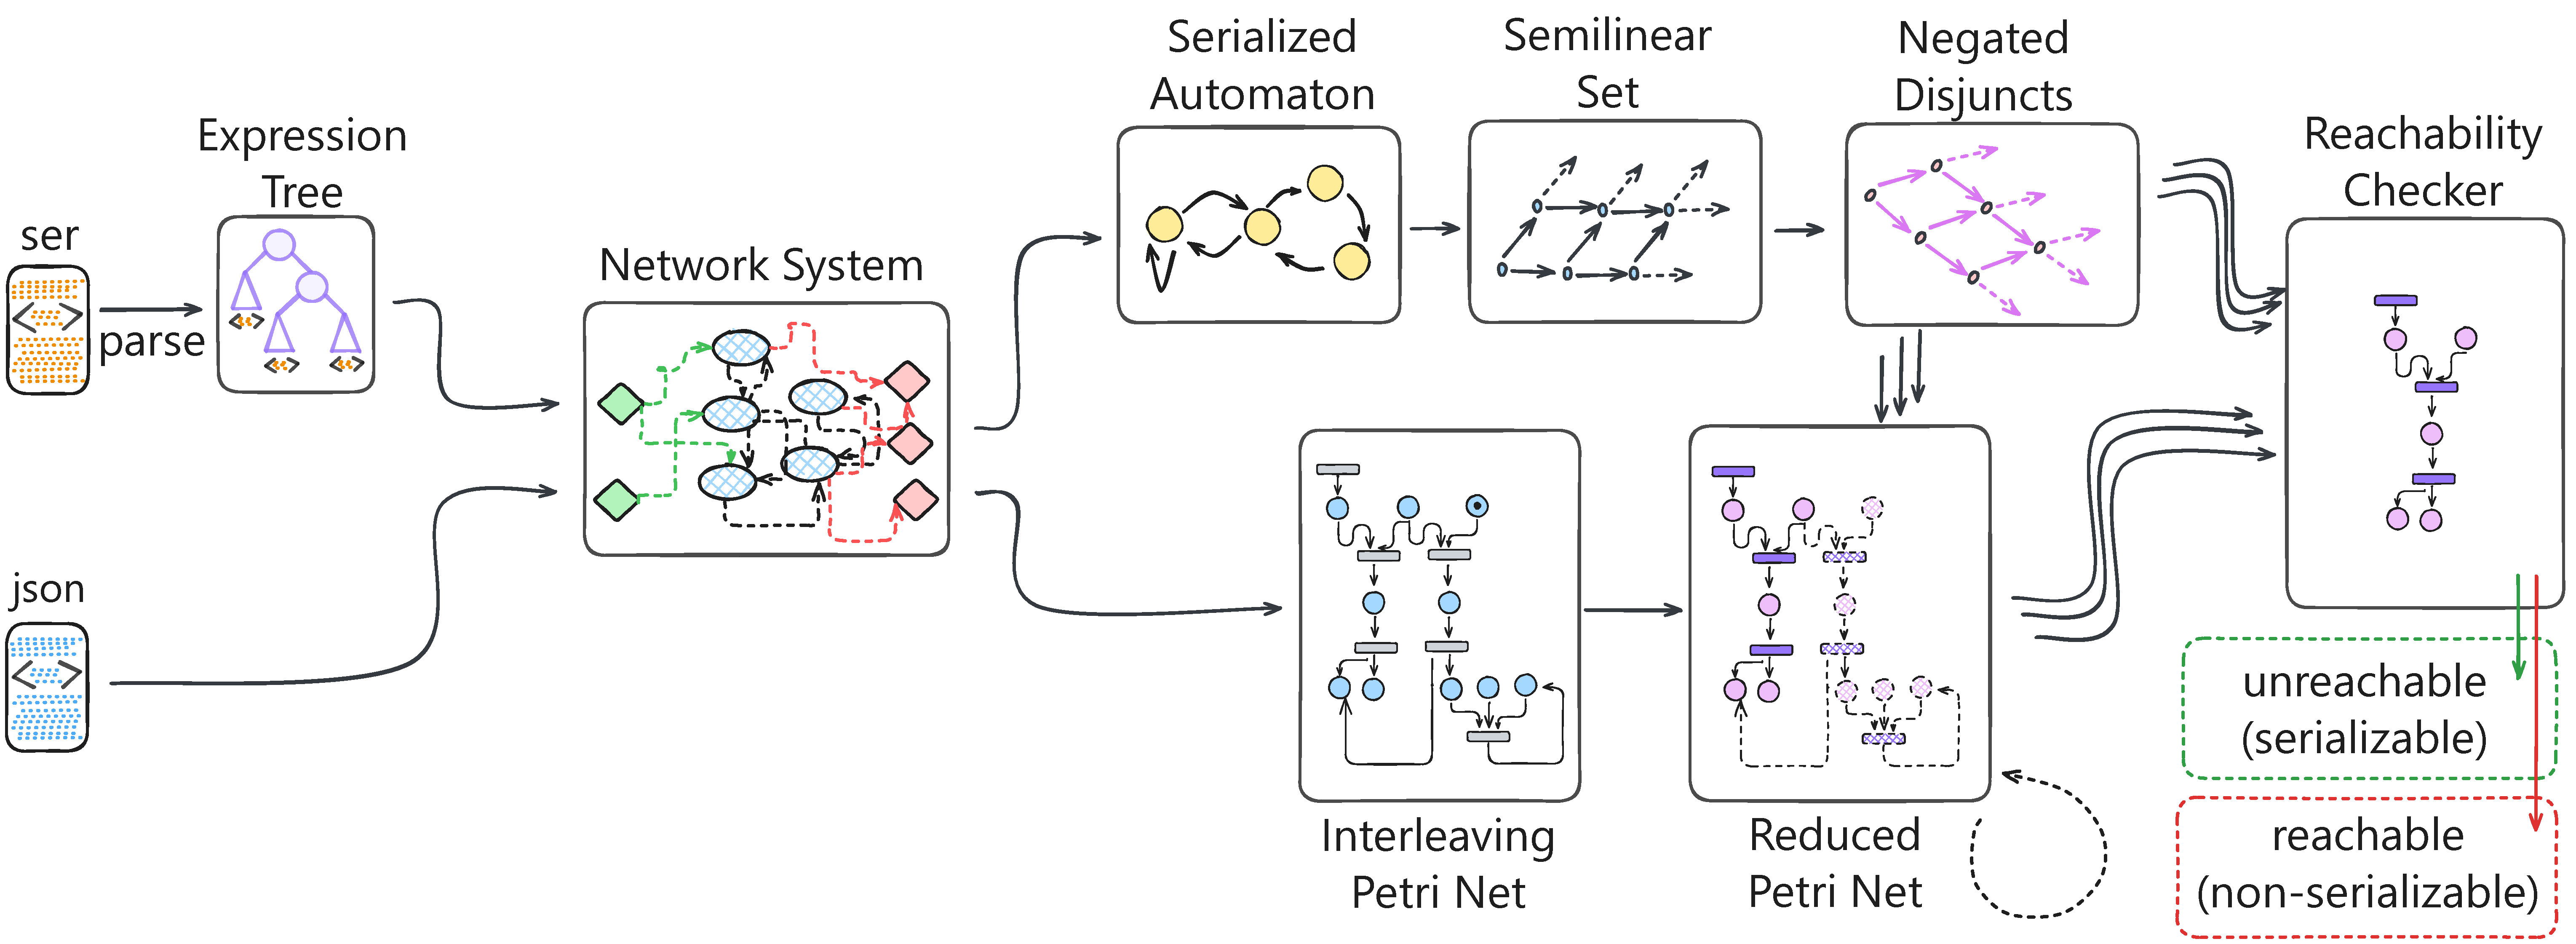
\includegraphics[width=1.0\textwidth]{plots/full_program_flow.pdf}
	\caption{Full program flow 
%		If the target set is unreachable --- a serializability proof is produced; otherwise, if it is reachable --- a counterexample trace is generated.
	(simplified, without backward arrows 
%	translating invariants (if serializable) or counterexample traces (if non-serializable) back 
	to the NS level).}
	\label{fig:full_program_flow}
\end{figure}


%\subsection{Optimizations}

%\paragraph{Bidirectional Pruning of the Petri Net}
%Before any heavy symbolic reasoning takes place, we apply bidirectional pruning on the underlying PN.  In the forward pass, we traverse from the initial marking to identify all places and transitions that could ever fire; in the backward pass, we traverse backward from any place that can influence a target constraint, and identify transitions and places that cannot contribute to reaching it.  By iteratively repeating forward passes and backward passes until convergence, we remove every component of the net that cannot both originate and contribute to the reachable target set.  This dramatically shrinks the net in practice, often converting an intractably large model into one small enough for exhaustive analysis.
%%
%We depict this in Fig.~\ref{fig:bidirectional_pruning}, and give a formal proof of correctness in Appendix~\ref{appendix:BidirectionalProof}.

%\paragraph{Redundant‐Constraint Elimination}
%When manipulating Presburger sets or their semilinear representations, it is common for some inequalities or disjuncts to add no new coverage beyond what other constraints already guarantee.  The redundant‐constraint elimination pass inspects each linear inequality and each disjunct in a disjunctive normal form, testing whether it is implied by the rest.  Any constraint or disjunct found redundant is dropped, ensuring that subsequent intersection, union, and projection operations work on the smallest necessary formula.  This streamlines the logic formula and prevents exponential blow‐up of case distinctions during solver invocations.
%
%Every time you build or star a semilinear set, you prune out any “period” vectors that are rendered useless by earlier steps:. nce you’ve accumulated a bunch of LinearSet components, you try to merge any that mathematically subsume one another:

%\paragraph{Generating Fewer Constraints}
%During set‐construction--- especially when introducing new existentially‐quantified variables or combining transition effects, we selectively avoid generating any marking that would strictly dominate an already‐seen solution.  In effect, whenever a candidate disjunct would yield a superset of an existing one, it is skipped entirely.  This ``generate‐less” heuristic stops the proliferation of large, overlapping regions in the semilinear description, trading off completeness of intermediate case‐enumeration for concise final representations.  In benchmarks with large state‐spaces, it can reduce the number of intermediate branches by orders of magnitude.

%in both the Regex and SemilinearSet Kleene-algebra instances. Concretely, instead of always building the full new structure and pruning it later, operations like union (plus) and concatenation (times) do a quick check for trivial cases and drop “zero” or “one” elements on the spo

%\paragraph{Executing Kleene Elimination in a Strategic Order:}
%When converting an NFA to a single regex, we pick the next state to eliminate by heuristically choosing the  state with the fewest incoming and outgoing edges.
%This optimization allows circumventing 
%overblown expressions resulting in naive translations, especially with regard to  Kleene closures (the “\(\mathsf{*}\)” operator).  Instead, we analyze the structure of sub-expressions under the various operators --- estimating their branching factor, and reorder them so that simpler, low‐branching components are expanded first.  This adaptive ordering often leads to early detection of fixed points or dead‐ends, preventing the combinatorial explosion that arises when complex loops are expanded prematurely.  




\subsection{Benchmark Overview} 
\label{subsec:benchmarks}
To the best of our knowledge, ours is the first and only tool to: (i) statically check serializability on \textit{unbounded} programs; and (ii) \textit{prove serializability holds}.
%
Thus, and due to lack of standard benchmarks for evaluating serializability, we 
assembled a suite of dozens of benchmarks (accompanying our artifact~\cite{ArtifactRepository}).
These include both serializable and non-serializable instances encoded in both \texttt{SER} and \texttt{JSON} formats, and covering a broad range of features, including arithmetic, locks, loops, non-determinism, and more (see an overview of all our benchmarks in Table~\ref{tab:benchmarks-all} of Appendix~\ref{appendix:full_results}.
%
We note that although the benchmarks themselves are not the main part of the paper, we believe they have merit on their own, due to their relevance to various real-world systems of interest.
%
Specifically, we wish to note our suite of benchmarks encoding \textit{networking \& system protocols} (see Table~\ref{tab:networking-benchmarks}), which include stateful firewalls, BGP routing programs, network monitors, and more --- 
%highlighting the serializability challenges inherent in real-world distributed programs.
%
%Here, we were motivated by 
as motivated by real-world concurrency problems in this domain. One such example is our \textit{routing-cycle benchmark} in software-defined networks, (motivated by~\cite{NaGhSa24}). Another real-world example is our \textit{snapshot isolation benchmark} (explained in Appendix~\ref{appendix:tour}), that was motivated by a real database bug, namely, duplicate-key errors~\cite{cockroach-issue-14099} in the \texttt{CockroachDB} system~\cite{cockroachdb-si-docs}, and the non-serializable behavior was automatically identified by our toolchain.
%
%Our benchmarks include both serializable and non-serializable instances, and their features and categorization appears in Table~\ref{tab:benchmarks-all}. 



%As there are no standard benchmarks for evaluating serializability, we wrote dozens of programs in our abstract NS language. These benchmarks span a wide range of complexity --- covering branching, looping constructs, arithmetic, non-deterministic choice, and multi-request workflows that manipulate both shared (global) variables and per-request (local) state. 
%
%We include both serializable and non-serializable instances and summarize the benchmarks' features and categorizations in Table~\ref{tab:benchmarks-all}. 
%
%In particular, our most sophisticated examples are drawn from realistic networking and system-protocol scenarios, including stateful firewalls, BGP routing, network monitoring, and more --- highlighting the serializability challenges inherent in real-world distributed programs.
%
%As there are no official benchmarks for evaluating serializability, we hand-coded dozes of programs in our abstract network-system language.
%%
%The benchmarks vary in the complexity, and have multiple features: branching, loops, arithmetic, non-determinism, and multiple requests and responses, operating on both shared (global) variables and per-request (local) variables.
%%
%The benchmarks include both serializable and non-serializable instances, as we summarize in Table.~\ref{tab:benchmarks-all}, based on a category and feature-wise breakdown.
%%
%Especially, we wish to note the final category of complex examples as motivated by real-world systems and networking programs.
%%
%These include a stateful firewall, BGP routing, network monitoring and additional examples.
%
%\begin{itemize}
%		
%	\item \todo{update benchmark overview and category names}
%	\item \textbf{Core expressions \& multi request workflows}: Benchmarks testing arithmetic, boolean, and simple control expression.
%	\item \textbf{Fred (mixed arithmetic)}: Mixed control and arithmetic transformations (Fred series).
%	\item \textbf{Stop (circular-increment) series}: Circular increment loops and variants.
%	\item \textbf{Concurrency \& locking loops}: Concurrent looping patterns with locking and tricky interactions.
%	\item \textbf{Non-deterministic choice \& randomness}: Random choice and non-deterministic branching benchmarks.
%	\item \textbf{Networking \& system protocols}: Networking protocols and system-level monitoring.
%	\item \textbf{JSON state-machine examples}: Example JSON-encoded state machine workflows.
%\end{itemize}
%
%
%
%The benchmarks differ in their complexity and in the various features pertaining to them --- branching, loops, randomness, multiple requests, etc. 
%



%\newpage
\section{Evaluation}
\label{sec:evaluation}

%\begin{enumerate}
%    \item Benchmarks (describe our benchmarks)
%    \item Results (total time, split out SMPT time from our rust code time)
%    \item Analysis of optimizations (how much time they save, petri net sizes, semilinear set sizes)
%    \item Limitations (examples we cannot solve, future work that would help)
%\end{enumerate}


\noindent
\textbf{Experimental setup.}
All experiments ran on a Lenovo ThinkPad P16s, with 16 AMD cores and 64 GB of RAM, running on a Linux Ubuntu 24.04.2 operating system.
%
%We plan on making all our code, benchmarks raw results publicly available with the final version of this paper.
%
We use \texttt{SMPT}~\cite{AmDa23} (built upon \texttt{Z3}~\cite{DeBj08}) as our backend Petri net model checker.
 %
Our code, benchmarks, and full experimental results are publicly available~\cite{ArtifactRepository}.



\subsection{Results}
We ran \toolname{} on all 47 benchmarks, out of which 27 are serializable, and the remaining 20 are non-serializable. 
For each benchmark, we measured the time for deciding the reachability query, as well as the overall time, including validation of the invariant proof (if serializable) or of the counterexample (if not serializable). These experiments ran in parallel on $16$ cores with all four optimizations and a \texttt{TIMEOUT} threshold of $500$ seconds.
%
Within this time limit, \toolname{} solved 26 of the 27 serializable benchmarks and 19 of the 20 non-serializable benchmarks (see summary in Table~\ref{tab:stats-summary} and the full results in Table~\ref{tab:benchmarks-all} of the appendix).
%
% As can be seen by our results (summarized in Table~\ref{tab:benchmarks-all}), withing this time limit, our tool fully solved 26/27 serializable benchmarks 
%and 19/20 non serializable benchmarks. 
%
The \textit{median} total runtime was $1{,}909$ ms across all benchmarks, and $2{,}238.50$ ms ($830$ ms) when  solely focusing on serializable (non-serializable) benchmarks.
%, as reported in Table~\ref{tab:stats-summary}.
%
The \textit{average} total runtime was $32{,}898.38$ ms across all benchmarks, and $25{,}530.69$ ms ($42{,}980.47$ ms) when solely focusing on serializable (non-serializable) benchmarks.
%
We also observe a clear runtime split based on serializability: 
%For serializable benchmarks, certificate validation takes much longer than proof generation. 
among non-serializable benchmarks, counterexample generation is much longer than validation, and dominates the runtime; whereas the opposite holds in non-serializable benchmarks. This is not surprising, as validating a given counterexample only requires a polynomial-time simulation of the network to confirm its feasibility.
%
%We also note that when analyzing the benchmarks based on their serializability, there is a clear difference in their average runtime --- while in the serializable benchmarks the validation of the certificate takes significantly longer than generating the certificate (i.e., the proof) --- in the non serializable benchmarks this trend is reversed, with the overall time being dominated by the generation of the counterexample. This of course is not surprising, as counterexample generation can be done in polynomial time by emulating our network system and checking that the final counterexample can indeed be attained.
%
%We report the full results in Table~\ref{tab:stats-summary} and Table~\ref{tab:benchmarks-all}.
%, and elaborate on the per-benchmark results in Table~\ref{tab:benchmarks-all}.


%\begin{table}[!htbp]
%	\centering
%	% Load the tabular from the external file:
%	\begin{table}[H]
	\centering
	\begin{tabular}{l r r r r}
		\toprule
		& \multicolumn{2}{c}{Average time (ms)} 
		& \multicolumn{2}{c}{Median time (ms)} \\
		\cmidrule(lr){2-3} \cmidrule(lr){4-5}
		Category
		& \shortstack{certificate\\generation}
		& total
		& \shortstack{certificate\\generation}
		& total \\
		\midrule
		Serializable      &   2{,}273 &  25{,}531 &  1{,}178 &  2{,}238 \\
		Not serializable  &  42{,}076 &  42{,}980 &   773 &   830 \\
		All               &  39{,}613 &  52{,}858 &   797 &  2{,}080 \\
		\bottomrule
	\end{tabular}
\end{table}

%	\caption{Average and median runtime. Values are rounded to the nearest integer, to reduce clutter. The \textit{total} column also includes the time for validation.}
%	\label{tab:stats-summary}
%\end{table}



%\begin{table}[H]
%	\centering
%	% Load the tabular from the external file:
%	\begin{table}[H]
	\centering
	\begin{tabular}{lrrrrrr}
		\toprule
		& \multicolumn{3}{c}{Average time (ms)} & \multicolumn{3}{c}{Median time (ms)} \\
		\cmidrule(lr){2-4} \cmidrule(lr){5-7}
		Category
		& \shortstack{certificate\\generation}
		& \shortstack{certificate\\validation}
		& total
		& \shortstack{certificate\\generation}
		& \shortstack{certificate\\validation}
		& total \\
		\midrule
		Serializable      &   2273 &  23257 &  25531 &  1178 &  1300 &  2238 \\
		Not serializable  &  42076 &    905 &  42980 &   773 &    78 &   830 \\
		All               &  39613 &  13244 &  52858 &   797 &   151 &  2080 \\
		\bottomrule
	\end{tabular}
\end{table}
%\caption{Average and median runtime. Values are rounded to the nearest integer, to reduce clutter.}
%\label{tab:stats-summary}
%\end{table}





%=== Overall ===
%Certificate running time:
%Average = 39613.23
%Median  = 797.00
%
%Certificate validation time:
%Average = 13244.32
%Median  = 151.00
%
%Total running time:
%Average = 52857.55
%Median  = 2080.00
%
%=== Serializable Only ===
%Certificate running time:
%Average = 2273.38
%Median  = 1178.00
%
%Certificate validation time:
%Average = 23257.31
%Median  = 1299.50
%
%Total running time:
%Average = 25530.69
%Median  = 2238.50
%
%=== Non-Serializable Only ===
%Certificate running time:
%Average = 42075.84
%Median  = 773.00
%
%Certificate validation time:
%Average = 904.63
%Median  = 78.00
%
%Total running time:
%Average = 42980.47
%Median  = 830.00
%
%=== Percentiles (Overall) ===
%Certificate running time percentiles:
%25th percentile = 553.50
%50th percentile = 797.00
%100th percentile = 502810.00
%
%Certificate validation time percentiles:
%25th percentile = 66.50
%50th percentile = 151.00
%100th percentile = 282370.00
%
%Total running time percentiles:
%25th percentile = 615.00
%50th percentile = 2080.00
%100th percentile = 503336.00
%
%=== Percentiles (Serializable) ===
%Certificate running time percentiles:
%25th percentile = 312.00
%50th percentile = 1178.00
%100th percentile = 9858.00
%
%Certificate validation time percentiles:
%25th percentile = 115.75
%50th percentile = 1299.50
%100th percentile = 282370.00
%
%Total running time percentiles:
%25th percentile = 456.50
%50th percentile = 2238.50
%100th percentile = 292228.00
%
%=== Percentiles (Non-Serializable) ===
%Certificate running time percentiles:
%25th percentile = 628.50
%50th percentile = 773.00
%100th percentile = 356195.00
%
%Certificate validation time percentiles:
%25th percentile = 50.00
%50th percentile = 78.00
%100th percentile = 15227.00
%
%Total running time percentiles:
%25th percentile = 707.00
%50th percentile = 830.00
%100th percentile = 356299.00





\begin{table}[htbp]
	\centering
	% Load the tabular from the external file:
	\begin{table}[H] 
	\centering
	\small
	% increase horizontal padding between columns
	\setlength{\tabcolsep}{5pt}
	\renewcommand{\arraystretch}{0.9}
	\begin{tabular*}{\textwidth}{@{\extracolsep{\fill}}%
			p{2cm}     % Benchmark
			c          % Serializable
			c c c c c c % Features
			r r        % Cert, Total
		}
		\toprule
		\textbf{Benchmark}
		& \textbf{Serializable}
		& \multicolumn{6}{c}{\textbf{Features}}
		& \multicolumn{2}{c}{\textbf{Runtime (ms)}} \\
		\cmidrule(lr){1-1} \cmidrule(lr){2-2} \cmidrule(lr){3-8} \cmidrule(lr){9-10}
		& 
		& If & While & \texttt{?} & Arith & Yield & Multi-req
		& Cert. & Total \\
		\midrule
		\texttt{banking (1)}          & \xmark      & \cmark & \cmark &        & \cmark & \cmark & \cmark & 59{,}312 & 74{,}539 \\
		\texttt{banking (2)}          & \greencmark & \cmark & \cmark &        & \cmark & \cmark & \cmark & \texttt{TIMEOUT} & \texttt{TIMEOUT} \\
		\texttt{routing (1)}      & \xmark      & \cmark & \cmark & \cmark & \cmark & \cmark & \cmark & 20{,}557 & 20{,}954 \\
		\texttt{monitor (1)}       & \xmark      & \cmark & \cmark & \cmark & \cmark & \cmark & \cmark & 6{,}859  & 7{,}047 \\
		\texttt{monitor (2)}       & \greencmark & \cmark & \cmark & \cmark & \cmark & \cmark & \cmark & 3{,}047  & 12{,}324 \\
		\texttt{firewall (1)}& \xmark      & \cmark &        & \cmark & \cmark & \cmark &       & 8{,}193  & 8{,}285 \\
		\texttt{firewall (2)}& \greencmark & \cmark &        & \cmark & \cmark &       &       & 6{,}886  & 252{,}752 \\
		\midrule
		\bottomrule
	\end{tabular*}
\end{table}

	\caption{Overview of benchmarks from the \textit{network \(\&\) system protocols} category. 
%	For our full benchmarks see Appendix~\ref{appendix:full_results}.
}
\label{tab:networking-benchmarks}
\end{table}


\subsection{Optimization Analysis}
\label{subsec:optimization-results}

%Next of our four optimizations, and analyzed their effect on the overall runtime and space resources.
%
%All experiments were run with a \texttt{TIMEOUT} value of $150$ seconds.


\subsubsection{Runtime optimization.}

We ran all benchmarks with each of the following six optimization configurations: 
(i) without any optimization (marked [\texttt{\textbf{\text{-}\text{-}\text{-}\text{-}}}] in Fig.~\ref{fig:timeout_cumulative_solved_log}); (ii) with bidirectional pruning (marked [\texttt{\textbf{\text{B}\text{-}\text{-}\text{-}}}]); (iii) with redundant constraint elimination (marked [\texttt{\textbf{\text{-}\text{R}\text{-}\text{-}}}]); (iv) with generation of fewer constraints (marked [\texttt{\textbf{\text{-}\text{-}\text{G}\text{-}}}]);
(v) with strategic Kleene elimination (marked [\texttt{\textbf{\text{-}\text{-}\text{-}\text{S}}}]);
and finally, (vi) with all optimizations altogether (marked [\texttt{\textbf{\text{B}\text{R}\text{G}\text{S}}}]).
%
The results of the aggregated runtimes are presented in Fig.~\ref{fig:timeout_cumulative_solved_log} and show that over $19\%$ more benchmarks are solved when using all optimizations compared to running without any optimization.
%
Not surprisingly, the best configuration is the one with all optimizations on. 
%
We also note that the best single-optimization configurations with regard to runtime are [\texttt{\textbf{\text{-}\text{-}\text{G}\text{-}}}] and [\texttt{\textbf{\text{B}\text{-}\text{-}\text{-}}}], solving over $74\%$ and $72\%$ of the benchmarks respectively. 
%
We also note that the two remaining optimizations, [\texttt{\textbf{\text{-}\text{R}\text{-}\text{-}}}] and [\texttt{\textbf{\text{-}\text{-}\text{-}\text{S}}}], performed slightly worse (although not significantly) than without the optimizations when counting overall timeouts.
%
However, when analyzing these configurations, it seems that there are instances in which each of these optimizations still \textit{strictly} improves runtime.
%
For example, there are instances (see \texttt{a3.ser} and \texttt{a7.ser} in Appendix~\ref{appendix:full_results}), in which the use of the redundant constraint optimization (  [\texttt{\textbf{\text{-}\text{R}\text{-}\text{-}}}])
affords a speedup of between $72.2\%$ and $85.2\%$ over the same benchmarks without this optimization.

\subsubsection{Space optimization.}
Our optimizations also reduce the space complexity of the two main components --- the Petri net and the semilinear set.

\noindent
(1) \textbf{Petri net.} Bidirectional pruning (Fig.~\ref{fig:petri_size_reduction}) 
eliminates the average number of places \textit{by roughly half} --- from $23.91$ down to $12.79$. This optimization proved even more effective on transitions, \textit{eliminating about two-thirds}: from $37.3$ down to $12.61$. 
%Note that the pre-pruning averages were computed over $47$ nets (one per benchmark), whereas the post-pruning averages span $224$ nets, since each pre-pruning net gives rise to a separate pruned net per each disjunct.  
%\\

\noindent
(2) \textbf{Semilinear sets.} We ran an ablation experiment in which we compared all optimizations against runs where each of the three semilinear optimizations (excluding pruning) was disabled. The redundant-constraint elimination ([\texttt{\textbf{\text{B}\textcolor{red}{-}\text{G}\text{S}}}]) and the fewer-constraint generation elimination ([\texttt{\textbf{\text{B}\text{R}\textcolor{red}{-}\text{S}}}]) \textit{drastically} reduced component counts, with the latter being especially effective in reducing the \textit{maximal} number of components to be up to $\mathbf{931\times}$ smaller, and the \textit{average} number of components to be up to $\mathbf{223\times}$ smaller (Table~\ref{tab:semilinear-size-reduction}), when compared to the baseline executions configured with all optimizations on ([\texttt{\textbf{\text{B}\text{R}\text{G}\text{S}}}]). 
%
For fairness, we measured only benchmarks completed under all configurations, excluding cases where semilinear sets exploded beyond $2^{30}$ components and timed out. Thus, our reported improvements actually \textit{understate} the true impact of these optimizations on memory. Such blowups, %especially common in state-machine benchmarks with NS loops, 
render even simple programs infeasible without these optimizations.
	
	
%\subsubsection{Space Optimization}
%
%Our optimizations also reduce the space complexity of the two main components --- the Petri Net and the semilinear set.
%
%\smallskip
%\noindent
%\textbf{Petri Net size reduction.}
%%
%With all optimizations enabled, we evaluated (Fig.~\ref{fig:petri_size_reduction}) the impact of our bidirectional pruning by comparing, across all benchmarks, the average number of places and transitions removed due to this optimization. On average, pruning reduced the number of places \textit{by roughly half} --- dropping from $23.91$ places before pruning to $12.79$ places afterward. Pruning proved even more effective on transitions, \textit{eliminating about two-thirds} of them: from $37.3$ transitions on average before pruning down to $12.61$ afterward. Note that the pre-pruning averages were computed over $47$ nets (one per benchmark), whereas the post-pruning averages span $224$ nets, since each pre-pruning net gives rise to a separate pruned net per each disjunct. 
%of our reachability query. 
%These results are summarized in Fig.~\ref{fig:petri_size_reduction}.

%When running our tool with all optimizations on, we analyzed the effect of our bidirectional pruning, This was done be counting the average number of places and transitions before and after pruning, on all benchmarks.
%%
%The pruning resulted in a reduction of about half the number of original places --- from $23.91$ places on average \textit{before} pruning to $12.79$ places on average \textit{after} pruning.
%%
%The bidirectional was even more effective in reducing the transitions, as demonstrated by a removing about two thirds of the transitions --- resulting in pruned Petri Nets with $37.30$ transitions on average \textit{before} pruning to $12.61$ transitions on average \textit{after} pruning.
%%
%We note that the averaging for the pre-pruning step was done on $47$ nets, once per each benchmark, while the averaging for the post-pruning step was done on $224$ nets, as each pre-pruning net can give rise to multiple post-pruning nets, one per each disjunct in our reachability query.
%%
%These results are presented in Fig.~\ref{fig:petri_size_reduction}.


%Number of values for 'Before' bars:          47
%Number of values for 'After' bars:           224
%Average number of places before pruning:     23.91
%Average number of places after pruning:      12.79
%Average number of transitions before pruning: 37.30
%Average number of transitions after pruning:  12.61






%\smallskip
%\noindent
%\textbf{Semilinear set size reduction.}
%%
%Finally, our last experiment batch analyzed the size reduction among the semilinear sets.
%%
%Towards this end, we ran all our benchmarks with all optimizations to serve as a baseline. 
%%
%Then, we analyzed the effect of the three semilinear-related optimizations, i.e., all but the bidirectional pruning. For each of these three optimizations, we ran the benchmarks with all optimizations \textit{except} the one checked.
%%
%%Table~\ref{tab:semilinear-size-reduction} include a summary of the results, when comparing the semilinear set size.
%%
%Specifically, we compare both the average and the maximal (i) number of components; and (ii) period vectors per each component, as summarized in Table~\ref{tab:semilinear-size-reduction}.
%%
%The redundant constraint elimination and the generate-less-constraints optimizations had a highly significant effect on the number of components, with the latter being especially effective in reducing the maximal number of components to be $931$ times more compact, as well as the average number of components to be $223$ times more compact, when compared to the baseline.
%%
%To ensure a fair comparison, we only measured benchmarks that were completed under every configuration, deliberately excluding any case where the optimized semilinear set exploded beyond $2^{30}$ components and timed out. By excluding these intractable runs, our reported performance improvements actually \textit{understate} the true impact of these optimizations. This explosive growth and the resulting timeouts are especially pervasive among our state-machine benchmarks due to loops in their NS, rendering even simple programs infeasible without optimizations.
%
%In fact, for both these optimizations are even more effective as, in order to conduct a fair comparison, we analyzed only benchmarks that terminated in all combinations, an hence we do not include cases in which these two optimizations rendered the original semilinear set intractable, due to having over $2^{30}$ components (!), hence timing-out and being excluded from the analysis.
%%
%This occurs pervasively in our state-machine benchmarks which have loops in their network systems --- and hence even simple programs of this category cannot be analyzed with respect to serializability.

%\todo{understand why this is related to loops in the NS}


\begin{center}
	\begin{minipage}[htbp]{0.48\textwidth}
		\centering
		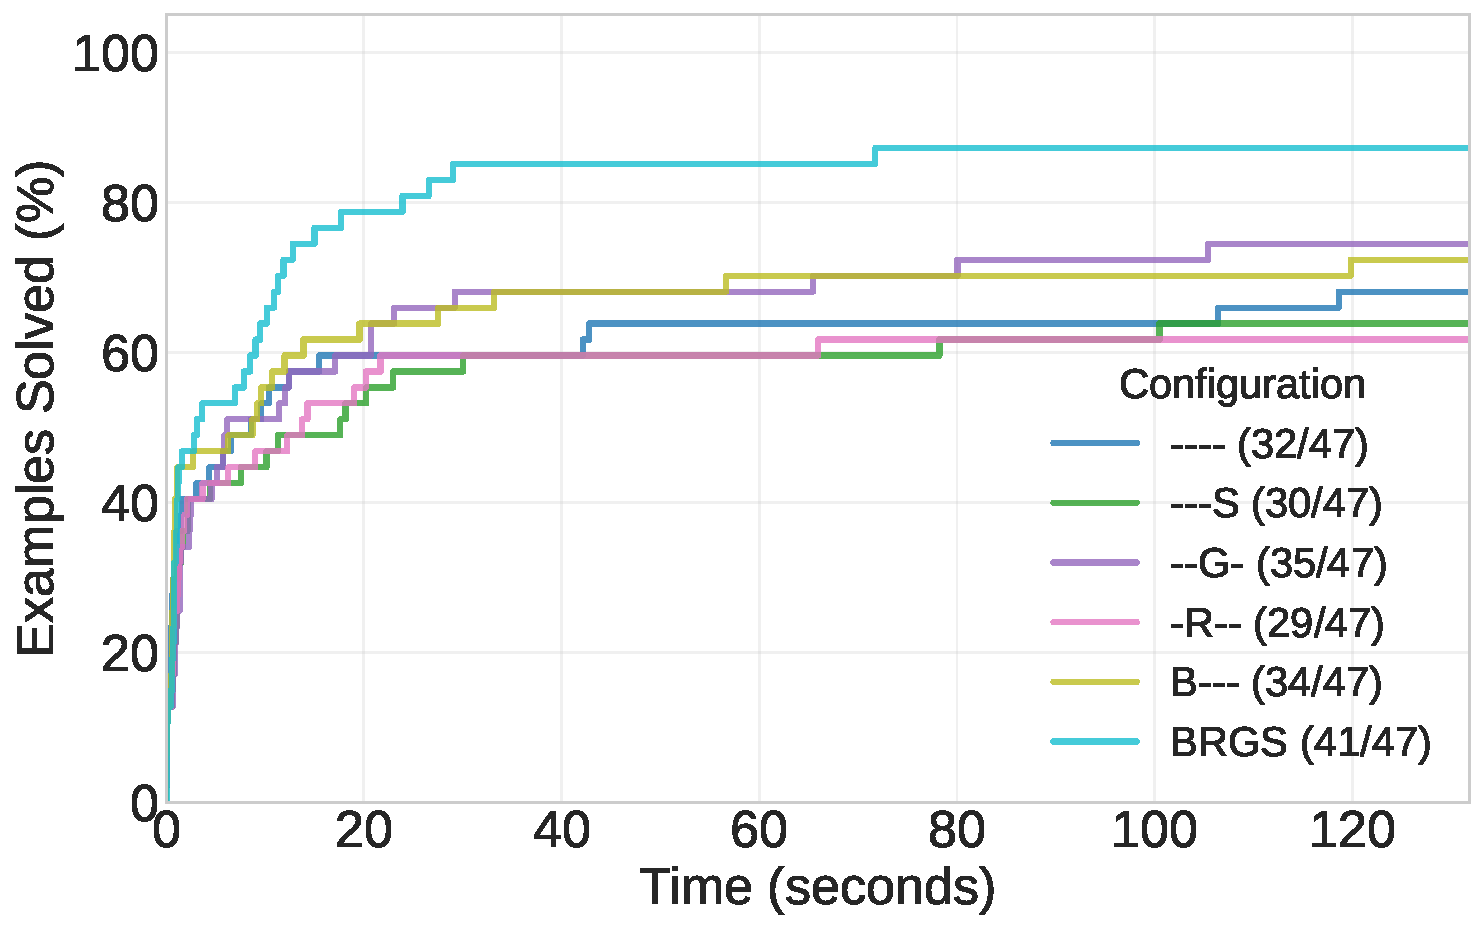
\includegraphics[width=\linewidth]{figures/cactus_plot.pdf}
		\captionof{figure}{Solved instances (\texttt{TIMEOUT} $150$ s).}
		\label{fig:timeout_cumulative_solved_log}
	\end{minipage}\hfill
	\begin{minipage}[htbp]{0.48\textwidth}
		\centering
		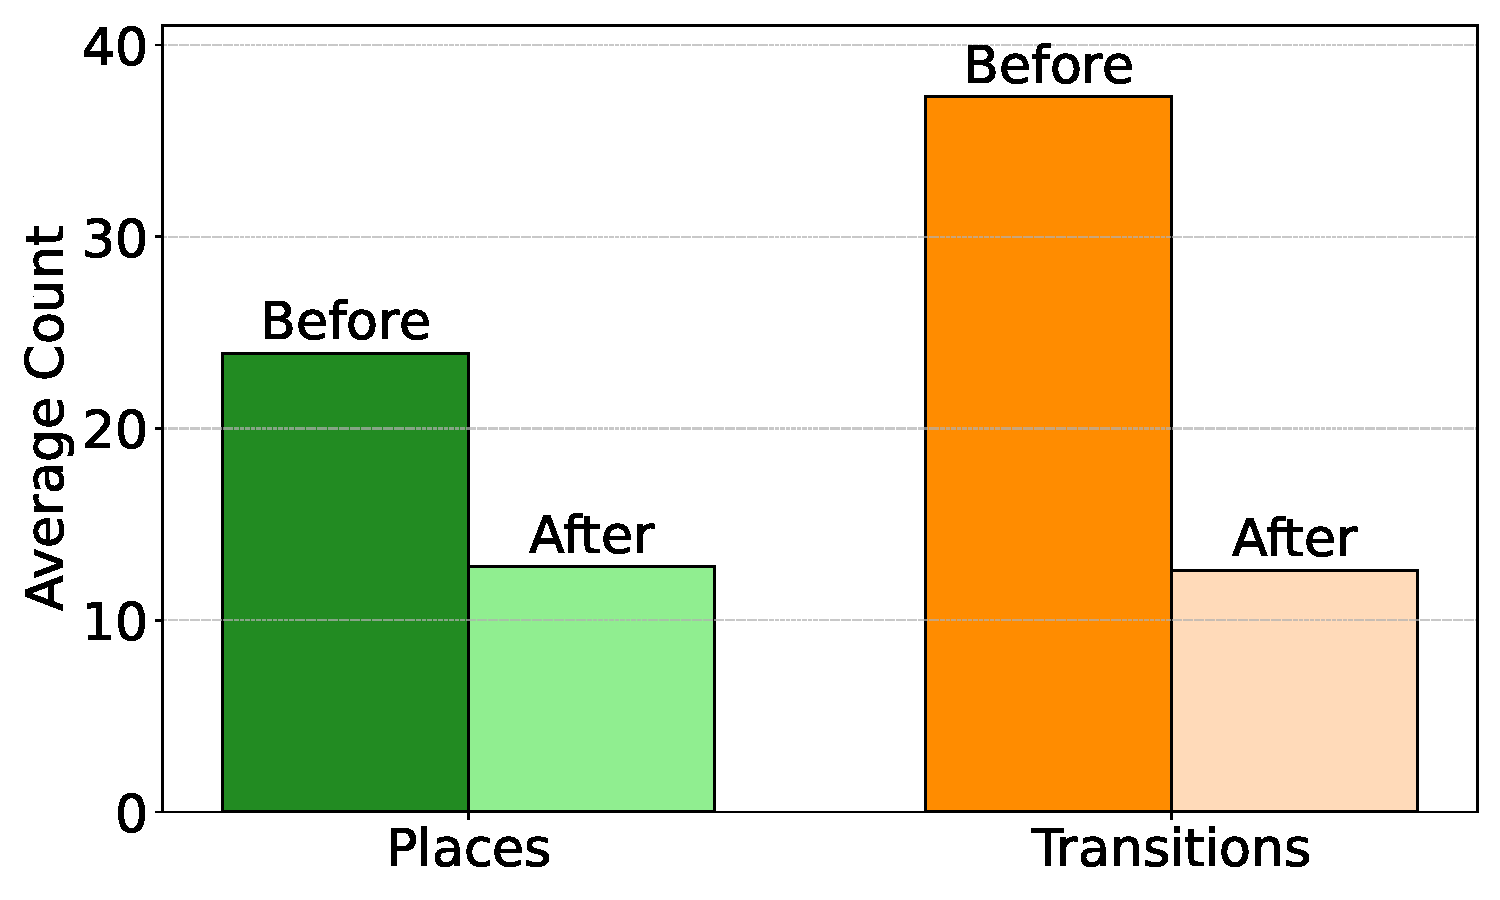
\includegraphics[width=\linewidth]{figures/petri_size_reduction_plot.pdf}
		\captionof{figure}{PN size reduction via pruning.}
			%(timeout 150 seconds)
			%.}
		\label{fig:petri_size_reduction}
	\end{minipage}
\end{center}

\begin{table}[!htbp]
	\centering
	\begin{minipage}[t]{0.48\linewidth}
	\centering
	\begin{table}[H]
	\centering
	\begin{tabular}{l r r r r}
		\toprule
		& \multicolumn{2}{c}{Average (ms)} 
		& \multicolumn{2}{c}{Median (ms)} \\
		\cmidrule(lr){2-3} \cmidrule(lr){4-5}
		Category
		& \shortstack{cert.}
		& total
		& \shortstack{cert.}
		& total \\
		\midrule
		\textcolor{ForestGreen}{Serializable}      &   2{,}273 &  25{,}531 &  1{,}178 &  2{,}238 \\
		\textcolor{red}{Not serializable}  &  42{,}076 &  42{,}980 &   773 &   830 \\
		All               &  39{,}613 &  52{,}858 &   797 &  2{,}080 \\
		\bottomrule
	\end{tabular}
\end{table}

	\caption{Runtime for generated certificates (\texttt{total} also includes validation).}
	%			Values are rounded to the nearest integer, to reduce clutter. 
	%The \textit{total} column also includes the time for validation.}
	% NOTE - this excludes the 2 non-terminating runs (artifact also includes TIMEOUTs I think)
	\label{tab:stats-summary}
	\end{minipage}\hfill
	\begin{minipage}[t]{0.48\linewidth}
	\centering
	\begin{table}[H]
	\centering
	\begin{tabular}{l c c c c}
		\toprule
		& \multicolumn{2}{c}{components} & \multicolumn{2}{c}{periods/component} \\
		\cmidrule(lr){2-3} \cmidrule(lr){4-5}
		& average & max & average & max \\
		\midrule
	\texttt{\text{B}\text{R}\text{G}\text{S}} & 2.91 & 22 & 1.33 & 4 \\
	\texttt{\text{B}\textcolor{red}{-}\text{G}\text{S}} & 8.79 & 194 & \textbf{1.64} & 11 \\
	\texttt{\text{B}\text{R}\textcolor{red}{-}\text{S}} & \textbf{651.41} & \textbf{20{,}484} & 1.28 & \textbf{15} \\
	\texttt{\text{B}\text{R}\text{G}\textcolor{red}{-}} & 2.91 & 22 & 1.35 & 4 \\
  \bottomrule
	\end{tabular}
\end{table}

	\caption{Semilinear set size reduction via optimizations (baseline is [\texttt{\text{B}\text{R}\text{G}\text{S}}]).}
	\label{tab:semilinear-size-reduction}
\end{minipage}
\end{table}

%\begin{table}[!htbp]
%	\centering
%	% Load the tabular from the external file:
%	\begin{table}[H]
	\centering
	\begin{tabular}{l c c c c}
		\toprule
		& \multicolumn{2}{c}{number of components} & \multicolumn{2}{c}{periods per component} \\
		\cmidrule(lr){2-3} \cmidrule(lr){4-5}
		& average & max & average & max \\
		\midrule
	all optimizations (baseline) & 2.91 & 22 & 1.33 & 4 \\
	without remove-redundant & 8.79 & 194 & \textbf{1.64} & 11 \\
	without generate-less & \textbf{651.41} & \textbf{20{,}484} & 1.28 & \textbf{15} \\
	without smart-kleene-order & 2.91 & 22 & 1.35 & 4 \\
  \bottomrule
	\end{tabular}
\end{table}

%	\caption{Semilinear set size reduction via optimizations.}
%	\label{tab:semilinear-size-reduction}
%\end{table}

%\todo{Limitations?}
%Examples we cannot solve, future work that would help

%\newpage

%\vspace{-5pt}



%\newpage

\section{Related Work}
\label{sec:related-work}

% from the CAV-2010 Vafeiadis paper (+ some other papers in our slack RW thread):
%
%1. model checking techniques - find violations, but do not prove correctness as they work on finite-state systems
%
%2. static (and specifically, shape) analysis techniques (sometimes) work on unbounded threads but ,any of these require linearization points (annotated manually or automatically). Also, a ``failed'' proof can indicate incorrect linearization.
%
%3. manual verification efforts

%\subsection{Notions of serializability.}
%\label{subsec:related:notions-of-serializability}
%\smallskip
%\noindent
%\textbf{Notions of serializability.}
%Serializability (or \emph{atomicity}) was
%first introduced by Eswaran et al.~\cite{EsGrKoTr76}, which can be viewed as a relaxtion of \emph{conflict serializability} 
%%--- a stricter property, 
%%that not only require that the final state of the system be attained by an equivalent serial execution, but also, that this equivalence be attained by reordering non-conflicting operations.
%%formalized by Eswaran et al.~\cite{EsGrKoTr76} as a correctness condition for transactional systems, introducing \emph{conflict serializability}, a stricter variant 
%%that requires equivalence to a serial 
%%schedule solely by reordering non-conflicting operations (e.g., two reads by 
%%different threads). 
%and \emph{Strict serializability} (SSR)~\cite{Pa79}. Herlihy and Wing~\cite{HeWe87,HeWi90} adapted these ideas to define \emph{linearizability} for concurrent data structures,
%% --- this can also be viewed as a case of SSR in 
%%which each transaction consists of a single action, operating on a single 
%%concurrent object~\cite{WaSt06a}.
%giving rise to additional consistency models~\cite{ZhChWa13, RaMeBrKoSi93, La78,AhNeBuKoHu95}, 
%%Subsequent variants include \emph{quasi-linearizability}~\cite{ZhChWa13} and \emph{predicate-wise serializability}~\cite{RaMeBrKoSi93}. Weaker models like 
%%\emph{causal consistency}~\cite{La78,AhNeBuKoHu95}, realized in systems such as \texttt{COPS}~\cite{LlFrKaAn11}, 
%inspiring extensive research on model-checking and complexity analyses~\cite{BoEnGuHa17,ZeBiBoEnEr19,LaBo20}.



%\todo{original}
%
%\subsection{Notions of serializability.}
%\label{subsec:related:notions-of-serializability}
%
%Serializability (also termed 
%\textit{atomicity}) was first formalized by Eswaran et al.~\cite{EsGrKoTr76} as 
%a 
%correctness condition for concurrent transactional systems. 
%Their work also introduced what was later referred to as \textit{conflict 
%serializability}, a stricter variant that requires equivalence to a serial 
%schedule solely by reordering non-conflicting operations (e.g., two reads by 
%different threads). 
%%
%\textit{Strict serializability} (a.k.a. SSR~\cite{Pa79}) is a stronger 
%consistency 
%notion in which an execution need not only be serializable but also respects 
%the real-time ordering of the transactions, i.e., it is not enough for the 
%interleaving to be equivalent to a serial one, but the serial execution must 
%also preserve the ordering of the transactions.
%%
%%Strict serializability:
%%
%%Guerraoui et al.~\cite{GuHeJoSi08} present a algorithm for model checking 
%%strict serializability fro two threads. The work was later 
%%extended~\cite{GuHeSi11}, to include a manual proof for an arbitrary number of 
%%threads.
%%
%%Konig and Wehrheim recently proved that it is possible to decide whether 
%%all executions of a program are strictly serializable, given that the 
%%transactions are live~\cite{KoWe21}.
%%
%Herlihy and Wing~\cite{HeWe87, HeWi90} defined \textit{linearizability} as a 
%similar notion to that of serializability, but adapted from transactional 
%programs 
%to concurrent data structures. In this setting, a linearizable data structure 
%is one for which every concurrent execution 
%with any operations manipulating it, appearing as if the operations occurred 
%atomically, while respecting real-time ordering and obeying the object's 
%specification. 
%%
%Equivalently, this can also be viewed as a case of strict serializability in 
%which each transaction consists of a single action, operating on a single 
%concurrent object~\cite{WaSt06a}.
%%
%Due to the similarity between serializability and linearizability, we cover 
%related work pertaining to both notions.
%%
%Zhang et al.~\cite{ZhChWa13} relaxed the notion of linearizability to 
%\textit{quasi 
%linearizability}, and put forth a method to identify violations thereof in 
%concurrent data structures.
%%
%Rastogi et al.~\cite{RaMeBrKoSi93} introduced the notion of 
%\textit{predicate-wise serializability} (PWSR), which preserves database 
%invariants 
%while permitting non-atomic transactions.
%%
%Other non-serializability-related notions focus on weaker consistency models, 
%and include Lamport’s \textit{causal 
%consistency}~\cite{La78}, which was later generalized to shared 
%memory~\cite{AhNeBuKoHu95} 
%and implemented in systems like 
%COPS~\cite{LlFrKaAn11}, while motivating extensive research on model checking and 
%complexity analysis~\cite{BoEnGuHa17,ZeBiBoEnEr19,LaBo20}. 


%\subsection{Deciding serializability and linearizability}

%\medskip
%\noindent
\textbf{Theoretical results.}
Serializability (or \emph{atomicity}) was
first introduced by Eswaran et al.~\cite{EsGrKoTr76},
%, which can be viewed as a relaxtion of \emph{conflict serializability} 
%and \emph{Strict serializability} (SSR)~\cite{Pa79}. 
later motivating Herlihy and Wing's~\cite{HeWe87,HeWi90} similar notion of \emph{linearizability} for concurrent data structures. 
%,
%giving rise to additional consistency models~\cite{ZhChWa13, RaMeBrKoSi93, La78,AhNeBuKoHu95}, 
%inspiring extensive research on model-checking and complexity analyses~\cite{BoEnGuHa17,ZeBiBoEnEr19,LaBo20}.
%
The \emph{membership problem} --- deciding if a specific interleaving is serializable --- is \texttt{NP}-complete~\cite{Pa79}, a result that was later extended to linearizability~\cite{GiKo97}, as well as to other consistency models~\cite{BiEn19}. 
%Likewise, membership for 
% 
%(and  
%is also \texttt{NP}-complete in general
% --- a result that was later 
%extended to \textit{collections}~\cite{EmEn18}).
The \emph{correctness problem} --- whether \emph{all} executions satisfy this criterion --- is \texttt{EXPSPACE} when threads are bounded~\cite{AlMcPe96} and undecidable otherwise~\cite{BoEmEnHa13}, though decidable for bounded-barrier programs (and hence, for serializability). Bouajjani et al.~\cite{BoEmEnHa18} further show that unbounded-thread linearizability for certain ADTs reduces to VASS coverability in \texttt{EXPSPACE}~\cite{Ra78}. The \toolname{} toolchain is, to our knowledge, the first to implement Bouajjani et al.’s serializability algorithm~\cite{BoEmEnHa13}, adapting it to distributed transactions, extending it with a proof certificate mechanism, and scaling it with various optimizations to multiple, real-world programs. 
%Furthermore, we harness research theoretical advancements in PN model checking and are the first to generate serializability proofs for arbitrary programs.

%\todo{original}
%\subsubsection{Theoretical Results}
%%
%The \textit{membership problem} of serializability, is deciding whether a 
%specific interleaving is serializable. This has been proven to be 
%\texttt{NP}-complete 
%by Papadimitriou~\cite{Pa79}, a result that was later extended~\cite{BiEn19} to 
%other consistency models.
%Regarding linearizability, the easier, membership problem is 
%\texttt{NP}-complete in 
%general, as proven by Gibbons and Korach~\cite{GiKo97}. Their result was later 
%extended to \textit{collections}~\cite{EmEn18}.
%%\guy{Mark could you check EmEn18?}
%%
%The \textit{correctness problem} on the other hand, is much harder, and 
%pertains to deciding whether \textit{all} executions of a program are 
%serializable.
%%
%While the correctness problem of linearizability is in 
%\texttt{EXPSPACE}~\cite{AlMcPe96} when bounding the number of threads, 
% Bouajjani et al.~\cite{BoEmEnHa13} proved that it is undecidable otherwise. 
% The authors also prove that the correctness problem of 
%linearizability becomes decidable on the fragment of finite-barrier programs. 
%As serializability can be viewed as a case in which there are no barriers, this 
%implies that serializability membership is in fact decidable. 
%%
%In follow-up work, Bouajjani et al. prove that linearizability is decidable 
%also 
%in the unbounded case for specific abstract data types~\cite{BoEmEnHa18}, in 
%which the authors rely on checking coverability in a Vector Addition System 
%with States (VASS), which was proven to be in \texttt{EXPSPACE}~\cite{Ra78}.
%%
%Our work can be viewed as the first tool to implement serializability proofs, 
%building upon the theoretical algorithm proposed by Bouajjani et 
%al.~\cite{BoEmEnHa13}. While our setting differs from theirs in various aspects 
%(e.g., we derive 
%the serial specification directly from the program and provide a correctness 
%proof; our setting is a transactional distributed system while their setting pertains to a single concurrent object, etc.), the core connection makes our work an implementation of their approach 
%in spirit. However, despite the theoretical foundation, the implementation 
%itself is the key novelty --- translating their algorithm into a practical, 
%scalable tool required significant advancements which are highly
%non-trivial, demanding various optimizations such as automatic invariant 
%inference, automaton minimization, and additional techniques to handle 
%unbounded systems efficiently. 

\medskip
\noindent
\textbf{Model checking and runtime verification.}
%
Runtime checks for serializability and conflict/view‐serializability were proposed by Wang and Stoller~\cite{WaSt06a,WaSt06b}.  
TLA logic~\cite{La94} can express various serializability forms~\cite{CoOlPnTuZu07}, however, such approaches~\cite{SoVaVi20,Ho24} remain restricted to bounded systems due to finite‐state tools (\texttt{TLC}, \texttt{Apalache}~\cite{YuMaLa99,KoKuTr19}).  
Heuristic or enumeration-based model checkers include \texttt{Line-up}~\cite{BuDeMuTa10} (built upon \texttt{CHESS}~\cite{MuQaBaBaNaNe08}), \texttt{LinTSO}~\cite{BuGoMuYa12}, \texttt{Violat}~\cite{EmEn19} and its schema precursor~\cite{EmEn18}, bridge‐predicate methods~\cite{BuNeSe11,BuSe09}, and PAT‐based refinement checking~\cite{LiChLiSuZhDo12,SuLuDoPa09,LiChLiSu09,Zh11}.  
Recent work includes \texttt{RELINCHE} for bounded linearizability~\cite{GoKoVa25}, \texttt{CDSSpec}~\cite{OuDe17} (for \texttt{C/C++11}), \texttt{Lincheck}~\cite{KoDeSoTsAl23}, and \texttt{SAT}‐based~\cite{BiHeCa09,ViWeMa15} approaches~\cite{BuAlMa07}.  
Symbolic testing~\cite{EmEnHa15} can expose violations of observational refinement~\cite{FiOhRiYa10,BoEmCoHa15}.  
Other checkers, e.g. \texttt{SPIN}/\texttt{PARGLIDER}~\cite{Fl04,VeYaYo09,Ho97,VeYa08}, depend on explicit linearization points, which are difficult to determine~\cite{VeYaYo09}.  
Overall, existing methods are typically incomplete, bounded, or assume prior knowledge.  
By contrast, our method covers unbounded threads and uniquely produces serializability certificates.



%\smallskip
%\noindent
%\textbf{Model checking and runtime verification}
%
%Wang and Stoller propose runtime checks for serializability and conflict/view‐serializability by recombining executions~\cite{WaSt06a,WaSt06b}. 
%TLA logic~\cite{La94} provides a formal specification to ensure only serializable (or conflict-serializable~\cite{CoOlPnTuZu07}) executions occur. While it can naturally express ``real” serializability via final‐state equivalence, existing TLA-based methods~\cite{SoVaVi20, Ho24} 
%are confined to bounded transaction systems, as TLA-based model checkers like \texttt{TLC} and \texttt{Apalache} ~\cite{YuMaLa99, KoKuTr19} cannot handle unbounded transaction counts.
%While TLA encodings can capture ``real'' serializability (based on final-state 
%equivalence), as well as conflict-serializability~\cite{CoOlPnTuZu07}, 
%are confined solely to bounded systems due to finite‐state tools like \texttt{TLC} and \texttt{Apalache}~\cite{YuMaLa99,KoKuTr19}. Heuristic and enumeration‐based model checkers include \texttt{Line-up}~\cite{BuDeMuTa10} (built upon \texttt{CHESS}~\cite{MuQaBaBaNaNe08}), \texttt{LinTSO} for TSO~\cite{BuGoMuYa12}, \texttt{Violat} (and its schema‐based predecessor)~\cite{EmEn19,EmEn18}, bridge‐predicate methods~\cite{BuNeSe11,BuSe09}, and PAT‐based refinement checking~\cite{LiChLiSuZhDo12,SuLuDoPa09,LiChLiSu09,Zh11}. 
%and RELINCHE for bounded linearizability~\cite{GoKoVa25}. 
%Golovin et al.~\cite{GoKoVa25} recently introduced \texttt{RELINCHE}, a model checker for bounded linearizability that limits the number of invocable operations.
%Additional tools include \texttt{CDSSpec} (with regard to the \texttt{C/C++ 11} memory model)~\cite{OuDe17}, \texttt{Lincheck}~\cite{KoDeSoTsAl23}, SAT‐based methods~\cite{BuAlMa07}. Others have put forth symbolic  testing methods~\cite{EmEnHa15} to identify violations of \textit{observational refinement} --- a property equivalent to linearizability in some settings~\cite{FiOhRiYa10, 
%	BoEmCoHa15}.
%Furthermore, checkers such as \texttt{SPIN}/\texttt{PARGLIDER} rely on explicit linearization points~\cite{Fl04,VeYaYo09,Ho97,VeYa08}, which are hard to identify~\cite{VeYaYo09}.
%
%Furthermore, the remaining aforementioned methods are incomplete, limited to finite threads, or assume prior knowledge.
 %
%Unlike these, our method affords complete coverage for unbounded threads and is also the only one to produce serializability certificates.
%\guy{The above point is a bit tricky because SMPT is not complete..}



%\todo{original:}
%
%\subsubsection{Model checking and runtime verification}
%
%In a series of papers, Wang and Stoller put forth runtime techniques for 
%detecting serializability violations~\cite{WaSt06a} as well as conflict serializability and view-serializability~\cite{WaSt06b}. 
%%They do so 
%%by  checking whether a given execution can be recombined to generate 
%%non-serializable executions.
%%
%The expressive TLA logic~\cite{La94} is used to encode a 
%formal specification that validates whether only serializable executions (or 
%conflict-serializable~\cite{CoOlPnTuZu07}) always occur. 
%While TLA can naturally encode ``real'' serializability (based on final-state 
%equivalence), existing TLA-based approaches~\cite{SoVaVi20, Ho24} remain 
%limited to bounded transaction systems. This limitation stems from TLA/TLA+ 
%model checkers like \texttt{TLC} and \texttt{Apalache}~\cite{YuMaLa99, 
%KoKuTr19}, which require 
%finite-state verification and cannot handle unbounded transaction counts.
%%
%\texttt{Line-up}~\cite{BuDeMuTa10} (built on the \texttt{CHESS} model 
%checker~\cite{MuQaBaBaNaNe08}) includes a heuristic-driven technique that 
%searches for violations of linearizability by enumerating all possible 
%serializations. Similar to spirit is \texttt{LinTSO}~\cite{BuGoMuYa12} which 
%search for 
%linearizability violations in the Total Store
%Order (TSO) weak memory model.
%%
%\texttt{Violat}~\cite{EmEn19} is a tool that generates tests to identify 
%linearizability violations, by 
%enumeration linearizations efficiently, per program schema (instead of per 
%execution, as in~\cite{BuDeMuTa10}).This follows the authors' previous runtime verification technique~\cite{EmEn18}, which enumerates minimal visibility relations.
%%
%Additional model checking techniques were proposed by Burnim et 
%al.~\cite{BuNeSe11}, which are similar to Line-up~\cite{BuDeMuTa10} but based 
%on leveraging bridge predicates~\cite{BuSe09}. 
%%
%Liu et al.~\cite{LiChLiSuZhDo12} build upon \texttt{PAT}~\cite{SuLuDoPa09} 
%(also used 
%in~\cite{LiChLiSu09, Zh11}) and verify linearizability through the lens of 
%refinement checking optimization, for a finite number of threads.
%%
%%\guy{Mark, could you please check LiChLiSu09,Zh11}
%%
%Recently, Golovin et al.~\cite{GoKoVa25} presented \texttt{RELINCHE}, a model 
%checker for bounded-linearizability, in which a predefined number of operations 
%can be invoked.
%%
%Other automatic linearizability checking tools include the \texttt{CDSSpec} 
%specification checker under the C/C++ 11 memory model, and 
%\texttt{Lincheck}~\cite{KoDeSoTsAl23} for verifying linearizability in JVM by 
%Ou and 
%Demsky~\cite{OuDe17}. 
%%
%Burckhardt et al.~\cite{BuAlMa07} employ a SAT solver and check for 
%linearizability violations of specific client programs.
%%
%We also note the symbolic-reasoning-based (incomplete) approach by Emmi et 
%al.~\cite{EmEnHa15} to identify violations of \textit{observational refinement} 
%--- a property equivalent to linearizability in some settings~\cite{FiOhRiYa10, 
%	BoEmCoHa15}.
%%
%As far as we are aware, unlike our algorithm, none of these tools afford 
%complete coverage for the case of unbounded threads, nor afford a certificate for serializability.
%%
%Other model checking techniques (e.g.,~\cite{Fl04}) rely on specifying 
%\textit{linearization points} (a.k.a. commit points) --- points in which the 
%event occurs logically, and are challenging to identify~\cite{VeYaYo09}.
%%We note 
%%that identifying all such points can be quite challenging~\cite{VeYaYo09}.
%%
%These include the work of Vechev et al.~\cite{VeYaYo09}, built upon 
%\texttt{SPIN}~\cite{Ho97}, and extending the \texttt{PARGLIDER} 
%tool~\cite{VeYa08}.~\footnote{Vechev et al. can also apply their 
%technique without linearization points, but solely on bounded executions.}


\medskip
\noindent
\textbf{Static analysis.}
Static methods prove linearizability for bounded~\cite{AmRiReSaYa07,MaLeSaRaBe08} and unbounded systems~\cite{BeLeMaRaSa08,Va09,Va10}, but usually rely on heuristics or annotated linearization points (e.g.~\cite{DrPe14}).  
	Lian and Feng~\cite{LiFe13} propose a logic for non‐fixed points.  
%	Other approaches also depend on linearization points~\cite{OhRiVeYaYo10,ZhPeHa15,AbJoTr16}.  
	However, annotation‐based analyses~\cite{OhRiVeYaYo10,ZhPeHa15,AbJoTr16} may be inconclusive, as failures can stem from incorrect annotations rather than from true violations~\cite{BoEmCoHa15}.

\medskip
\noindent
\textbf{Manual proofs and specific data types.}
Tasiran~\cite{Ta08} proves serializability for \texttt{Bartok-STM}, while Colvin et al.~\cite{CoGrLuMo06} use I/O automata for list‐set linearizability.  
	Simplifications exist for specific data structures~\cite{BoEmEnMu17,FeEnMoRiSh18}.
%	, and verification has been pursued with~\cite{CoGrLuMo06} or without~\cite{DoGrLuMo04} proof assistants.  
	Other notable linearizability results include Wing and Gong's~\cite{WiGo93} on unbounded FIFO/priority queues, Chakraborty et al.~\cite{ChHeSeVa15} on queues, and Cerný et al.’s \texttt{CoLT} for linked heaps (which is complete only under bounded threads~\cite{CeRaZuChAl10}).  
	Bouajjani et al.~\cite{BoEnWa17} introduce a recursive priority‐queue violation detector, akin to their stack/queue methods~\cite{BoEmEnHa18}.

\medskip
\noindent
\textbf{Further approaches.}
Other strategies include testing~\cite{WiGo93,PrGr12,PrGr13,EmEn17,Lo17}, theorem proving~\cite{CoDoGr05,DeScWe11}, and the use of additional verification frameworks~\cite{BoEmEnMu17,FeEnMoRiSh18,EnKo24}.



%\smallskip
%\noindent
%\textbf{Static analysis}
%%
%Static techniques prove linearizability for bounded~\cite{AmRiReSaYa07,MaLeSaRaBe08} and unbounded~\cite{BeLeMaRaSa08,Va09,Va10} systems, but typically depend on heuristics or annotations of linearization points as well. Lian and Feng~\cite{LiFe13} offer a logic that handles non‐fixed points. Additional techniques that rely on linearization points include~\cite{OhRiVeYaYo10,ZhPeHa15,AbJoTr16}. 
%However, annotation‐based checkers and analyses are inconclusive, since failures may reflect incorrect annotation rather than true violations~\cite{BoEmCoHa15}.


%\todo{original:}
%
%\subsubsection{Stataic analysis}
%
%Static analysis techniques may prove linearizability for the 
%bounded~\cite{AmRiReSaYa07, BeLeMaRaSa08, MaLeSaRaBe08} and unbounded 
%cases~\cite{BeLeMaRaSa08, Va09, 
%	Va10}, but typically rely on heuristics and the manual/automatic annotation 
%	of 
%linearization points. 
%%
%Lian and Feng~\cite{LiFe13} propose a sound program logic that can prove 
%linearizability with non-fixed linearization points.
%%
%Other techniques that depend on linearization points 
%include~\cite{OhRiVeYaYo10, ZhPeHa15, AbJoTr16}. 
%%
%%\guy{Mark can you take a look at Va10, LiFe13, and ZhPeHa15?}
%%
%We note that both the model-checking techniques (e.g.,~\cite{CeRaZuChAl10}) and 
%the static analysis techniques which rely on linearization points are 
%inconclusive, as any failed proof can be due to incorrect annotation of the 
%linearization points~\cite{BoEmCoHa15}.
%%
%\smallskip
%\noindent
%\textbf{Manual proofs and specific data types}
%
%Tasiran~\cite{Ta08} proved serializability of the \texttt{Bartok STM}, and Colvin et al.~\cite{CoGrLuMo06} showed list‐set linearizability via I/O automata. 
%%
%Other methods demonstrate that in some cases, proofs can be simplified for specific data structures to which certain properties hold~\cite{BoEmEnMu17,FeEnMoRiSh18}.
%%
%Additional verification attempts of linearizability have been presented both 
%with~\cite{CoGrLuMo06} and without~\cite{DoGrLuMo04} the use of 
%proof assistants.
%%
%Wing and Gong~\cite{WiGo93} established linearizability for unbounded FIFO and priority queues, and Chakraborty et al.~\cite{ChHeSeVa15} developed a queue‐checking technique. Cerný et al.’s CoLT checks singly‐linked heap objects, however, this method is complete only for bounded threads~\cite{CeRaZuChAl10}. Bouajjani et al.~\cite{BoEnWa17} present a recursive priority‐queue violation detector, akin to their stack and queue methods~\cite{BoEmEnHa18}.
%
%
%\todo{original}
%
%\subsubsection{Manual proofs and results for specific data types}
%
%Tasiran~\cite{Ta08} proved serializability of the \texttt{Bartok STM}, and 
%Colvin et 
%al.~\cite{CoGrLuMo06} prove that a list-based set algorithm is linearizable by 
%simulating the observed behavior with input/output automata.
%%
%%\guy{Mark could you take a 2nd look at CoGrLuMo06? Not sure if this is 
%%considered manual. One paper which I put in the slack channel mentioned that it 
%%semiautomatically verifies linearizability of an implementation.}
%%
%Other methods demonstrate that in some cases, proofs can be simplified for specific data structure to which certain properties hold~\cite{BoEmEnMu17, FeEnMoRiSh18}.
%%
%Additional verification attempts of linearizability have been presented both 
%with (e.g.~\cite{CoGrLuMo06}) and without (e.g.~\cite{DoGrLuMo04}) the use of 
%proof assistants.
%%
%Linearizability has also been proven for specific data types. For example. 
%Wing and Gong~\cite{WiGo93} prove it for  (unbounded) FIFO queues, (unbounded) 
%priority queues and other data structures. Chakraborty et al.~\cite{ChHeSeVa15} 
%later provided a method for checking linearizability of queue-based algorithms, 
%without the use of linearization points. Cern{\`y} et al.~\cite{CeRaZuChAl10} 
%present \texttt{CoLT}, a model checker for linearizability of singly-linked 
%heap-based 
%objects. However, their approach is complete only with regard to a bounded 
%number of threads. 
%%
%Bouajjani et al.~\cite{BoEnWa17} present a recursive algorithm for identifying 
%linearizability violations in priority queues (based on register automata), in 
%a method similar to the one for finding linearizability violations in stacks 
%and (regular) queues~\cite{BoEmEnHa18}.
%%

%\smallskip
%\noindent
%\textbf{Additional approaches.}
%%
%Additional approaches include  testing~\cite{WiGo93,PrGr12,PrGr13,EmEn17,Lo17}, theorem‐proving~\cite{CoDoGr05,DeScWe11}, and more~\cite{BoEmEnMu17,FeEnMoRiSh18,EnKo24}.

%
%\todo{original}
%\subsubsection{Additional approaches}
%
%%
%Some methods combine multiple approaches, e.g., Shacham et 
%al.~\cite{ShBrAiSaVeYa11} use dynamic analysis to identify 
%violations of linearizability in concurrent data structures, and combine it 
%with a manual proof when their technique did not find a violation.
%%
%Other techniques attempt to generate tests for linearizability~\cite{WiGo93, 
%PrGr12, PrGr13, EmEn17}. For example, 
%Lowe~\cite{Lo17} presents a testing framework for linearizability by randomly 
%generating histories and subsequently testing if they are 
%linearizable.
%%
%There has also been ample research in technique for linearizability  and simplifying proofs for data structures pertaining ~\cite{BoEmEnMu17, FeEnMoRiSh18, EnKo24} 
%%
%Other techniques for linearizability proof include the use of theorem provers, 
%e.g.~\cite{CoDoGr05, DeScWe11} and proof assistance techniques~\cite{EnKo24}.
%
%\guy{Mark EnKo24 is the OOPSLA paper, is it legit to cite it as a proof assistance technique?} 
%Additional related work includes~\cite{BoEmEnMu17, FeEnMoRiSh18, EnKo24}.
%
%EnKo24: OOPSLA paper (Mark) trying to formalize and prove existing reduction techniques, and introduce a new abstraction for splitting linearizability checking scenarios (cases) and check if they covers all the checks. They don't actually check linearizability but say there it can help other checkers

%FeEnMoRiSh18 simplify proofs for some types of data structures

%BoEmEnMu17 also show that proof can be simplified sometimes 

%
%\subsection{Deciding conflict serializability}
%
%%\todo{original:} 
%
%\smallskip
%\noindent
%\textbf{Runtime enforcement.}
%Although conflict serializability is a more conservative measure than 
%serializability, it is easier for database schedulers to enforce during 
%runtime, either by \textit{pessimistic} locking approaches~\cite{BeHaGo87}, or 
%\textit{optimistic} approaches~\cite{KuRo81, BuMo06}, both ensuring  acyclicity in the conflict graph --- a necessary and 
%sufficient condition for conflict serializability. 
%However, by ignoring program semantics, they can reject executions that are serializable despite conflict cycles.
%
%%However, 
%%because these approaches \textit{ignore program semantics}, these may 
%%incorrectly reject executions that, although not conflict-serializable, are 
%%still valid serializable executions.
%%i.e., have the same result as a serial 
%%execution. 
%%
%%We note that the subject matter of this work is around the notion of (``real'') 
%%serializability, which takes 
%%into account the program semantics, and regards whether the final result of the 
%%program can be attained by a serial execution.
%%
%
%\smallskip
%\noindent
%\textbf{Theoretical results.}
%From the theoretical perspective, Alur et al.~\cite{AlMcPe96} established that the 
%correctness problem for conflict serializability is decidable (and in 
%\texttt{PSPACE}) 
%for bounded transaction systems. Bouajjani et al.~\cite{BoEmEnHa13} later 
%proved that decidability also holds in the unbounded case (and is \texttt{EXPSPACE}-complete). Their key insight reveals that while the conflict 
%graph 
%becomes infinite, cycle detection, and thus conflict serializability, is 
%independent of the transaction count. 
%%
%%By modeling transactions via Vector Addition Systems (equivalent to Petri 
%%Nets), they provide a finite framework for analyzing infinite behaviors. This 
%%approach inspired our use of Petri Nets to capture Int(S).
%%
%
%\smallskip
%\noindent
%\textbf{Approaches and techniques.}
%%
%Dynamic and monitoring‐based methods for checking conflict serializability, include Farzan and Mahusudan’s bounded monitoring~\cite{FaMa08}, Flanagan et al.’s \texttt{Velodrome}~\cite{FlFrYi08}, and other dynamic approaches include~\cite{FlFr04,XuBoRa05,WaSt06a,CoOlPnTuZu07,EmMaMa10,SiMaWaGu11a}. Hatcliff et al. leverage \texttt{Bogor} with Lipton’s mover theory~\cite{HaRoDw04,Li75}, while Elmas et al. use mover‐based program rewriting~\cite{ElQaSeSuTa10}. 
%Nagar and Jagannathan~\cite{KaJa18} presented an 
%automatic static analysis technique to find violations of conflict 
%serializability.
%Sinha et al. developed an incomplete predictive analysis technique, building on Sinha and Malik’s runtime checker~\cite{SiMaWaGu11b,SiMa10}, and Von Praun and Gross offer an unsound static checker~\cite{VoGr04}. Type-system approaches appear in~\cite{FlQa03,FlFrLiQa08}. 
%Brutschy et al.~\cite{BrDiMuVe17} present a dynamic analysis algorithm and a 
%tool that checks whether a given program execution is conflict serializable, in 
%an eventually consistent data store. A follow-up work~\cite{BrDiMuVe18} 
%further bridges these concepts by statically detecting 
%non-(conflict)-serializable behaviors in causally consistent databases.
%Conflict serializability has also been studied under weak memory models~\cite{EnFa16}.

%
%\todo{original:}
%
%\subsubsection{Approaches and techniques}
%
%Various works focus on checking conflict serializability, e.g., Farzan and 
%Mahusudan~\cite{FaMa08} present a monitoring-based decision procedure for 
%conflict serializability of a bounded number of operations, and Flanagan et 
%al.~\cite{FlFrYi08} present \texttt{Velodrome} --- a dynamic analyzer for 
%conflict 
%serializability. Additional dynamic approaches include~\cite{FlFr04, XuBoRa05, 
%WaSt06a, CoOlPnTuZu07, EmMaMa10, SiMaWaGu11a} and others.
%%
%%Other works~\cite{XuBoRa05} have also put forth techniques to automatically 
%%detect conflict-serializability violations.
%%
%Hatcliff et al.~\cite{HaRoDw04} demonstrate the use of the \texttt{Bogor} model 
%checker~\cite{RoDwHa03} and check atomicity w.r.t. Liptopn's reduction theory 
%of left/right movers~\cite{Li75} (which is reminiscent of 
%conflict-serializability).
%%
%Elmas et al.~\cite{ElQaSeSuTa10} also use the notion of movers and present an 
%(incomplete) technique to prove linearizability by iteratively rewriting an 
%input program.
%%
%%\guy{Mark can you please check out ElQaSeSuTa10}
%%
%Nagar and Jagannathan~\cite{KaJa18} presented an 
%automatic static analysis technique to find violations of conflict 
%serializability.
%%
%Sinha et al.~\cite{SiMaWaGu11b} present a sound and incomplete predictive 
%analysis technique for detecting violations of conflict serializability, 
%following the previous work of Sinha and Malik~\cite{SiMa10} which put forth a 
%runtime conflict serializability checker.
%%
%Von Praun and Gross~\cite{VoGr04} present an unsound static analysis technique 
%for identifying potential atomicity violations. Additional static analysis 
%techniques are based on type systems, e.g.~\cite{FlQa03, FlFrLiQa08}.
%%
%Brutschy et al.~\cite{BrDiMuVe17} present a dynamic analysis algorithm and a 
%tool that checks whether a given program execution is conflict serializable, in 
%an eventually consistent data store. In a follow-up work~\cite{BrDiMuVe18} 
%further bridges these concepts by statically detecting 
%non-(conflict)-serializable behaviors in causally consistent databases.
%%
%%Rinetzky et al.~\cite{RiBoRaSaYa} present a conservative static analysis 
%%techniques for verifying view-serializability on specific program sub-types.
%%
%%\guy{Mark, please see my masked comment on RiBoRaSaYa. Do we need to mention 
%%	them?}
%%
%We also note that conflict serializability has been studied in relation to weak 
%memory models~\cite{EnFa16}.
%%







% Specifically, our implementation leverages \texttt{SMPT}~\cite{AmDa23}, a 
% state-of-the-art Petri Net model checker that combines SMT-solving with 
% structural invariants~\cite{AmBeDa21, AmDaHu22}. At a high level, SMPT 
% formulates reachability as satisfiability queries (dispatched to the 
% \texttt{Z3} 
% solver~\cite{DeBj08}) while curtailing the search space~\footnote{As far as we 
% aware, the only two sound reachability solvers for unbounded Petri Nets are 
% \texttt{KReach}~\cite{DiLa20} and \texttt{SMPT}~\cite{AmDa23}. Although only 
% \texttt{KReach} is claimed as possibly complete, we decided in our 
% implementation to use \texttt{SMPT} as it was 
% reported~\cite{Am23} that \texttt{KReach} is unable to solve various 
% reachability 
% problems. 
% Still, our Petri Nets are encoded in the standard \texttt{.nnet} format, and 
% the property file is encoded in the standard \texttt{.XML} format --- in order 
% for our tool to be compatible with off-the-shelf solvers.
% }.
%
%We refer the reader to a survey by Esparza and Nielsen~\cite{EsNi94} (recently republished in~\cite{EsNi24}) for a comprehensive summary of additional decidability results pertaining to Petri Nets.
%
%Finally, we believe that our various, nontrivial optimizations, and first and 
%foremost --- the automatic invariant inference, are interesting in their own, 
%allowing the speedy termination of queries that otherwise timed-out. 

 
 






%Serializability first introduced by Eswaran et al.~\cite{EsGrKoTr76}. It is the first to put forth serializability as a correctness condition for concurrent transaction execution.
%The paper also covers conflict serializability --- a strictly stronger consistency property than serializability, that does not only require that the final state of the system be attained by an equivalent serial execution, but also, that this equivalence be attained by allowing only specific (``non-conflicting'') operations to be reordered.
%%
%Papadimitriou~\cite{Pa79} proved that it is NP-hard to decide whether even the history of a single interleaving is serializable. 
%%
%Moreover, although conflict serializability is more conservative measure than serializability, it is easier to enforce during runtime by various approaches. 
%%
%These approaches are typically categorized as either \textit{pessimistic} locking approaches, e.g, 2-Phase Locking~\cite{BeHaGo87}, or alternatively --- \textit{optimistic} locking approaches, e.g., Optimistic Concurrency Control (OCC)~\cite{KuRo81, BuMo06}.
%%
%
%Furthermore, most work, both in theory and in practice, focuses on proving theorems on conflict serializability, due to is being more straightforward, and corresponding to the programs dependency graph, and \textit{without taking the actual semantics into account}.
%%
%Alur et al.~\cite{AlMcPe96} cover the complexity for deciding conflict serializability, given a bound on the number of transactions. 
%%
%This work was later continued by Bouajjaniet al.~\cite{BoEmEnHa13}, which demonstrate that the problem of deciding whether a program with an \textit{unbounded} number of transaction is conflict serializable, is also decidable and is EXPTIME-complete. The authors show that although the conflict graph in such a case is infinite (and hence, infeasible to traverse) --- conflict serializability can still be decided as the size of the cycle (if it exists), surprisingly, does not depend on the number of transactions. The authors also emulate multiple transactions in a shared memory system with a Vector addition system, and equivalent object to a Petri Net. We took inspiration by defining a Petri Net to capture Int(S). 
%
%In another line of work, there is an attempt to \textit{directly} validate (regular, non-conflicting) serializability by encoding this specification in the highly expressive \textit{Logic of Temporal Actions} (TLA)~\cite{La94}. 
%%
%Although, unlike the aforementioned works, TLA itself allows encoding serializability in the original form (focusing on the final state of the variables), such works~\cite{SoVaVi20, Ho24} cannot validate this behavior for an \textit{unbounded} number of transactions. This is because, although TLA/TLA+ allow encoding the properties of interest, their model checkers (such as TLC and Apalache)~\cite{YuMaLa99, KoKuTr19} can only operate on a finite and predefined number of transactions.
%%
%Although these works present important progress, as far as we are aware, our work is the first to decide serializability for all executions, based solely on the program semantics and final state, regardless of read/write conflicts. Furthermore, ours is the first to handle the unbounded case; and to supply an actual end-to-end implementation.
%
%
%Other work relaxes the (strong) consistency notion of serializability and allows weaker consistency notions. For example, Rastogi et al.~\cite{RaMeBrKoSi93}
%introduce \textit{predicate-wise serializability} (PDSR) --- a relaxation of serializability in which transactions might not be atomic, but are still required to maintain some desired database consistency predicate
%%
%Furthermore, other relaxations focus on weaker consistency models. One such model is causal consistency, which was put forth by Lamport~\cite{La78}, en extended to shared memory systems as \textit{causal memory}~\cite{AhNeBuKoHu95}. (include causal + consistency, designed in COPS~\cite{LlFrKaAn11}). The have been a plethora of works on model checking systems that adhere to causal consistency, and hence the complexity of such procedures~\cite{BoEnGuHa17,ZeBiBoEnEr19,LaBo20}.
%%
%We also note that some work combine various consistency notions. These include the recent work by Brutschy et al.~\cite{BrDiMuVe18}, who put form a method to statically detect non-serializable executions on top of
%causally-consistent databases.
%
%
%
%
%Our work also builds upon both theoretical literature, as well as practical results, pertaining to Petri Nets~\cite{Mu89, Es96, Re12}.
%%
%Firstly, our undecidability result is based on a classic result by Hack~\cite{Ha76, HaThesis76}, showing that, given two Petri Nets, it is undecidable to answer whether they have equivalent reachability sets. Hack based his result on the work of Rabin (which was never published). These undecidability results follow from a series of reductions, originating from Hilbert's 10th problem, i.e., deciding if a Diophantine polynomial has an integer root (a problem that was proved undecidable by Matijas{\'e}vi{\v{c}}~\cite{Ma70}).
%%
%Later, Jan{\v{c}}ar~\cite{Ja95} proved this result by demonstrating that Petri Nets can simulate 2-counter Minsky Machines~\cite{Mi67}, which are universally computable and hence undecidable. Moreover, Jan{\v{c}}ar strengthened the original result and proved that reachability equivalence is undecidable even for Petri Nets with five unbounded places~\cite{Ja95}.
%%
%
%Our decision procedure itself is based on an algorithm for deciding whether a given marking is reachable, for a Petri Net.
%%
%Mayr~\cite{Ma81} was the first to put forth an algorithm for this problem 
%given a (potentially, unbounded) Petri Net (note that for bounded case this is 
%straightforward, as you can enumerate all reachable markings.)
%%
%Mayr's reachability algorithm was later improved and simplified by Kosaraju~\cite{Ko82}, and then again by Lambert~\cite{La92}.
%%
%Very recently, this problem was also proven to be Ackermann complete~\cite{CzWo22}, implying that, although decidable, it is practically infeasible to solve on large nets.
%%
%Furthermore, these theoretical algorithms have inspired various tools, such as K-Reach~\cite{DiLa20}, DICER~\cite{XiZhLi21}, MARCIE~\cite{HeRoSc13}, and others. 
%%
%Specifically, our tool employs SMPT~\cite{AmDa23}, a state-of-the-art Petri Net reachability tool, which employs an SMT-based approach~\cite{AmBeDa21, AmDaHu22}. SMPT curtails the search space by reducing the reachability problem to a satisfiability query (that is subsequently dispatched to the Z3 solver~\cite{DeBj08}) and inferring invariants on the net's structure.
%%
%We refer the reader to a survey by Esparza and Nielsen~\cite{EsNi94} (recently republished in~\cite{EsNi24}) for a comprehensive summary on additional decidability results pertaining to Petri Nets.


%\vspace{-1.5pt}



\section{Discussion}
\label{sec:discussion}

%\subsection{Conclusion}


%




%\subsection{Limitations}
%\smallskip
%\noindent
\textbf{Limitations.}
Petri-net reachability is \texttt{Ackermann}-complete~\cite{CzWo22}, so some complex benchmarks time out despite optimizations. Our current backend (\texttt{SMPT}~\cite{AmDa23}) may also miss existing proofs. Finally, the NS model assumes request/response interactions and does not cover streaming, callbacks, or partial responses.

%\subsection{Future Work}
\smallskip
\noindent
\textbf{Future Work.}
We are developing polyhedral reductions~\cite{AmBeDa21,Be87,BeLeDa20} to verify reduced nets and lift proofs to the original. We also plan to support richer communication models beyond independent clients.
%\todo{old}
%
%\paragraph{Scalability.}
%
%Our evaluation shows that some benchmarks still time out.
%To improve \textit{scalability}, we are developing both theory and implementation of \textit{polyhedral reductions}~\cite{AmBeDa21} --- that are structural reductions~\cite{Be87,BeLeDa20} of the form $(N_1, m_1) \vartriangleright_E (N_2, m_2)$ where $N_2$ is a simpler Petri Net and $E$ is a formula enabling reconstruction of $N_1$'s state space from $N_2$'s. This would let us verify the reduced net and lift proofs back to the original net.
%
%\guy{Nicolas are you sure about the next sentence? Do you have an explanation or a "negative proof"?}
%
%Furthermore, we note that polyhedral reductions are the only type of structural reduction for which such a conversion is possible.
%
%We are developing both theory and implementation for this extension.
%
%\todo{Limitations?}
%Examples we cannot solve, future work that would help
%To conclude..
%
%
%
%In another axis, we aim to \textit{extend our framework to more diverse communication patterns.}
%\paragraph{Extensions to diverse communication models.}
%Currently, clients act independently: each issues a request, receives a response, then verification is centralized. Stronger models allow inter-client communication or partial orderings (Lamport’s \textit{happens-before}~\cite{La78}); weaker ones forbid post-response communication or permit only limited summaries. Addressing such settings will require decentralized certification or streaming proofs under communication constraints. Extending our framework along these axes would capture a broader class of practical distributed-system guarantees.


%\paragraph{Extensions to diverse communication models.}
%
%Our current framework assumes that clients act independently --- each submits a request, receives a response, and only afterward collaborates to verify (in a centralized manner) whether the combined outcomes are serializable. However, in a stronger model, clients may communicate during execution or enforce partial ordering of their interactions. More generally, this can be formalized via Lamport’s \textit{happens‐before} relation over request/response pairs~\cite{La78}. 
%%
%In contrast, a weaker model disallows communication --- in which case clients either cannot communicate after receiving responses or may only share limited summaries. Jointly deciding serializability in this setting will require decentralized certification techniques or streaming proofs that respect tight communication constraints. 
%%
%By extending our theory and tool along these two axes, we aim to cover a broad spectrum of practical distributed‐system guarantees, that are more complex and match broader, real-world scenarios.

%
%
%
%\todo{Different notions of serializability}
%\begin{itemize}
%    \item \todo{Current notion: clients independently submit a request and get a response, and later they all get together and see if what they got was serializable}
%    \item \todo{Stronger: clients are not independent, or sequentially execute some parts. General: we have some happens-before on the requests/responses}
%    \item \todo{Weaker: the clients cannot communicate with each other afterwards to determine whether what they got was serializable, or they can only communicate in a limited way}
%    \item \todo{Infinite / unbounded executions}
%\end{itemize}



\smallskip
\noindent
\textbf{Conclusion.}
We presented the first implemented tool that verifies serializability for unbounded concurrent systems and generates proof certificates, bridging theory and practice with a decision procedure, key optimizations, and an evaluation on diverse, realistic benchmarks.



\newpage

{
	\bibliographystyle{abbrv}
	\bibliography{references}
}

\newpage
%\newpage
%% Appendix
\appendix


\section{Tour of Examples}
\label{appendix:tour}


Next, we will walk through a series of examples, in varying levels of complexity. Each example will demonstrate different aspects of serializable vs. non-serializable programs.
%
The first examples are relatively basic, while the last examples have higher complexity and are motivated by real-world programs, e.g., BGP routing policy updates.
%
Each thread is spawned any number of times (and at any point in time) by a \textit{request} from the user, marked {\color{ForestGreen}$\blacklozenge_\text{req}$}. The request executes, and eventually returns a \textit{response}  {\color{red}$\blacklozenge_\text{resp}$}.
%
For instance, in the three examples presented in \Cref{sec:introduction} (Listings~\ref{lst:MotivatingExample1Ser},~\ref{lst:MotivatingExample2NonSer}, and~\ref{lst:MotivatingExample3Ser}), there is a single type of request {\color{ForestGreen}$\blacklozenge_\text{main}$} and (up to) two types of responses {\color{red}$\blacklozenge_0$}, {\color{red}$\blacklozenge_1$}.
% 
We analyze serializability through the lens of such {\color{ForestGreen}$\blacklozenge_\text{req}$}/{\color{red}$\blacklozenge_\text{resp}$} pairs. Specifically, the programs in Listings~\ref{lst:MotivatingExample1Ser} and~\ref{lst:MotivatingExample3Ser} only induce pairs of the type {\color{ForestGreen}$\blacklozenge_\text{main}$}/{\color{red}$\blacklozenge_1$}, while the program in Listing~\ref{lst:MotivatingExample2NonSer} can also induce {\color{ForestGreen}$\blacklozenge_\text{main}$}/{\color{red}$\blacklozenge_0$}, as formulated by our Network System framework (see \Cref{sec:problem-definition}). 
%
We depict global variables with upper-case characters, while local variables (per each request) are depicted with lower-case ones.
%
Unless explicitly stated otherwise, all global and local variables are initialized to 0.
%
The symbol \texttt{?} depicts a nondeterministic choice between 0 and 1. All other constructs (\texttt{while}, \texttt{yield}, and \texttt{if}) have their standard interpretation, and are based on the \toolname{} semantics covered in Appendix~\ref{appendix:ser-semantics}.

\subsection{Example 1}

%\subsubsection{Example 1}

We start with a basic example, describing a single request {\color{ForestGreen}$\blacklozenge_\text{A}$}, a single local variable (\texttt{x}) per each request; and a single global variable (\texttt{FLAG}) shared among all in-flight requests. 
%
In Listing~\ref{lst:BasicSer}, an in-flight request assigns to \texttt{x} the value of \texttt{FLAG} (hence, initially, \texttt{[x:=0]}). Then, the request non-deterministically chooses whether to \texttt{yield} or to flip the value of \texttt{x}. Subsequently, \texttt{FLAG} is assigned 1 and the value of \texttt{x} is returned as the response to request {\color{ForestGreen}$\blacklozenge_\text{A}$}. 
%
Note that the presence of the \texttt{else} branch renders the program serializable, as intuitively, 
for any interleaving that modifies \texttt{x} via the \texttt{if} branch, there exists a corresponding serial execution in which the \texttt{else} branch is taken, yielding an equivalent outcome.
%
However, this changes in  Listing~\ref{lst:BasicNonSer},
%
%
%\begin{wrapfigure}{r}{0.62\textwidth}
%	\vspace{-0.5\intextsep} % tighten top
%	\centering
%	\begin{minipage}[t]{0.25\textwidth}
%		\begin{lstlisting}[caption={Serializable},label={lst:BasicSer},numbers=none]
%request A: 
%    x := FLAG
%
%    if (?):
%        yield
%    else:
%        x := 1 - x
%
%    FLAG := 1
%    return x
%		\end{lstlisting}
%	\end{minipage}\hspace{1.2em}% <-- small gap here
%	\begin{minipage}[t]{0.25\textwidth}
%		\begin{lstlisting}[caption={Not serializable},label={lst:BasicNonSer},numbers=none]
%request A: 
%    x := FLAG 
%
%    if (?): 
%        yield
%    // no else
%
%
%    FLAG := 1 
%    return x
%		\end{lstlisting}
%	\end{minipage}
%	\vspace{-0.9\intextsep} % tighten bottom
%\end{wrapfigure}
%
%
in which there is no \texttt{else} branch --- an update that makes the program non-serializable.
%
Now, any serial execution will have \textit{at most one} pair of {\color{ForestGreen}$\blacklozenge_\text{A}$}/{\color{red}$\blacklozenge_0$} (this is in fact the first request, returning the original zero-initialized value of \texttt{FLAG}).
%
As the first request also assigns \texttt{[FLAG:=1]} before terminating, any subsequent request in a serial run will assign \texttt{[x:=1]} and hence, will return only responses of {\color{red}$\blacklozenge_1$}. 
%, and $(i-1)$ pairs of {\color{ForestGreen}$\blacklozenge_\text{A}$}/{\color{red}$\blacklozenge_1$}.
%
%
%
%Any serial execution will match the first request {\color{ForestGreen}$\blacklozenge_\text{A}$} the response {\color{red}$\blacklozenge_0$} (as $[x:=FLAG]$, which is initially 0). 
%
%
%
%
%Differently put, for any serial execution with i requests --- we have exactly one (first) request/response pair {\color{ForestGreen}$\blacklozenge_\text{A}$}/{\color{red}$\blacklozenge_0$}, and $(i-1)$ pairs of {\color{ForestGreen}$\blacklozenge_\text{A}$}/{\color{red}$\blacklozenge_1$}.
%
%\noindent
However, given that the first request can also \texttt{yield}, it is possible for another request to concurrently run the program after the first request yields and before it resumes. This, in turn, will allow more than one request to assign \texttt{[x:=0]}, and hence, for example, we can attain \textit{multiple} {\color{ForestGreen}$\blacklozenge_\text{A}$}/{\color{red}$\blacklozenge_0$} pairs. Thus, Listing~\ref{lst:BasicNonSer} is not serializable.
%\noindent
%\begin{minipage}[t]{0.30\textwidth}
%	\begin{lstlisting}[caption={Serializable},
%		label={lst:BasicSer}]
%request A: 
%    x := FLAG
%
%    if (?):
%        yield
%    else:
%       x := 1 - x
%
%    FLAG := 1
%    return x
%	\end{lstlisting}
%\end{minipage}
%\hfill
%\begin{minipage}[t]{0.30\textwidth}
%	\begin{lstlisting}[caption={Not serializable},
%		label={lst:BasicNonSer}]
%request A: 
%    x := FLAG 
%
%    if (?): 
%        yield
%    // no else
%
%
%    FLAG := 1 
%    return x
%	\end{lstlisting}
%\end{minipage}%


%\todo{original:}

%\vspace{2em}
%example - 2

% Second row
\noindent
\begin{minipage}[t]{0.45\textwidth}
	\begin{lstlisting}[caption={Serializable},
		label={lst:BasicSer},numbers=none]
request A: 
    x := FLAG
    if (?):
        yield
    else:
        x := 1 - x
    FLAG := 1
    return x
	\end{lstlisting}
\end{minipage}
\hfill
\begin{minipage}[t]{0.45\textwidth}
	\begin{lstlisting}[caption={Not serializable},
	label={lst:BasicNonSer},numbers=none]
request A: 
    x := FLAG 
    if (?): 
        yield
    // no else
	
    FLAG := 1 
    return x
		\end{lstlisting}
\end{minipage}%

\subsection{Example 2}

%\subsubsection{Example 2}
The following program pairs have a single global variable (\texttt{X}), and two requests --- {\color{ForestGreen}$\blacklozenge_\text{incr}$} which increments \texttt{X} by 1, and {\color{ForestGreen}$\blacklozenge_\text{decr}$} which decrements \texttt{X} by 1. Both programs have loops that guarantee that \texttt{X} will always be between 0 to 3, otherwise the \texttt{while} loop will yield ad infinitum. Both requests return the value of \texttt{X} after updating it.
%
In the first case, Listing~\ref{lst:FredSer} presents a serializable program, due to the absence of any \texttt{yield} between the increment/decrement of \texttt{X} and its return. Equivalently, in each of the requests, the update of \texttt{X} and the returned value can be thought of as \textit{a single atomic execution}.
%
However, in Listing~\ref{lst:FredNonSer}, we add an additional \texttt{yield} (and a local variable \texttt{y}), occurring in each of the requests, between the update of \texttt{X} and its return.
%
This change allows requests of the same type to update \texttt{X} to the same value ---  resulting in outputs such as
$\{{\color{ForestGreen}\blacklozenge_\text{incr}}/{\color{red}\blacklozenge_\text{1}},{\color{ForestGreen}\blacklozenge_\text{incr}}/{\color{red}\blacklozenge_\text{2}},{\color{ForestGreen}\blacklozenge_\text{incr}}/{\color{red}\blacklozenge_\text{3}},{\color{ForestGreen}\blacklozenge_\text{decr}}/{\color{red}\blacklozenge_\text{2}},{\color{ForestGreen}\blacklozenge_\text{decr}}/{\color{red}\blacklozenge_\text{2}}\}$ which cannot be obtained in any serial execution.

%
%
%
%  incr/1
%incr/3
%incr/2
%(decr/2)^2
 %

%\vspace{2em}
%\newpage
%example - 3

% Third row
\noindent
\begin{minipage}[t]{0.45\textwidth}
	\begin{lstlisting}[caption={Serializable},
		label={lst:FredSer},numbers=none]
request incr: 
    while (X == 3):
        yield


    X := X + 1
    return X		

request decr: 
    while (X == 0): 
        yield


    X := X - 1
    return X
		\end{lstlisting}
\end{minipage}
\hfill
\begin{minipage}[t]{0.45\textwidth}
	\begin{lstlisting}[caption={Not serializable},
		label={lst:FredNonSer},numbers=none]
request incr:
    while (X == 3):
        yield
    y := X
    yield
    X := y + 1
    return X		

request decr: 
    while (X == 0):
        yield
    y := X
    yield
    X := y - 1
    return X
		\end{lstlisting}
\end{minipage}
	
\subsection{Example 3}
%\subsubsection{Example 3}	
%\todo{continue}	
%example - 6

The next example (see Listing~\ref{lst:ComplexWhileNonSer}) has a global variable \texttt{X} and, for each in-flight request, a local variable \texttt{i}. The {\color{ForestGreen}$\blacklozenge_\text{flip}$} request flips \texttt{X} (initialized to 0); the {\color{ForestGreen}$\blacklozenge_\text{main}$} request attempts to decrement \texttt{i} five times.
%
%It is straightforward to observe that the program in Listing~\ref{lst:ComplexWhileSer} is trivially serializable, as there are no yields.
%
Any serial execution cannot induce a response {\color{red}$\blacklozenge_1$}, 
as it will have a single request in-flight, with \texttt{X} being either 0 or 1. Thus, exactly one of the \texttt{while} loops will run indefinitely, prohibiting any {\color{ForestGreen}$\blacklozenge_\text{main}$}/{\color{red}$\blacklozenge_1$} pairs.
%
%Specifically, in any serial execution of requests, the local i variable is either 0 or 1, and hence --- serial execution do no produce any request/response pairs.
%
To prove that the program is not serializable, we show that an interleaving \emph{can} result in a non-empty set of outputs. 
%
%However, some interleavings can allow the program to output a response {\color{red}$\blacklozenge_1$}. 
%
Specifically, given at least \texttt{[i=5]} interleavings of in-flight {\color{ForestGreen}$\blacklozenge_\text{flip}$} requests, it is possible for a {\color{ForestGreen}$\blacklozenge_\text{main}$} request to terminate and bypass all \texttt{while} loops, something that cannot occur in any serial execution.
%
%Here is some text that will flow around the code listing. You can introduce the snippet and then let the text wrap naturally alongside it.

\vspace{1em}  
\begin{wrapfigure}{r}{0.38\textwidth}
	  \vspace{-1em}  % pull the top of the figure up by 1em
	\centering
	\begin{lstlisting}[caption={Not serializable},label={lst:ComplexWhileNonSer},numbers=none]
request flip: 
    X := 1 - X 

request main:
    i := 5
    while (i > 0):
        while (X == 0):
            yield
        while (X == 1):
            yield
        i := i - 1

    return 1        
	\end{lstlisting}
\vspace{-0.5em}  % tighten space at bottom of the listing
\end{wrapfigure}
\vspace{1em}  % space below the wrapfigure; change as needed

%This paragraph will flow to the left of the listing. Continue writing your explanation or narrative here, and the text will neatly wrap around the code block on the right. You can add as much text as you like, and LaTeX will handle the wrapping automatically.

%\bigskip

%If you need to reference the listing elsewhere, use \texttt{\textbackslash ref~\{lst:ComplexWhileNonSer\}} to point to it, e.g., Listing~\ref{lst:ComplexWhileNonSer}.

% Second row
%\noindent
%\begin{minipage}[t]{0.45\textwidth}
%	\begin{lstlisting}[caption={Serializable},
%		label={lst:ComplexWhileSer}]
%		    request flip: 
%		        X := 1 - X 
%		    
%		    request main:
%		        i := 5
%		        while (i > 0):
%		            while (X == 0):
%		                pass
%		            while (X == 1):
%		                pass
%		            i := i - 1
%		        
%		        return 1       
%				\end{lstlisting}
%\end{minipage}%
%\hfill
%\begin{minipage}[t]{0.45\textwidth}
%	\begin{lstlisting}[caption={Not serializable},
%		label={lst:ComplexWhileNonSer}]
%		    request flip: 
%		        X := 1 - X 
%		
%		    request main:
%		        i := 5
%		        while (i > 0):
%		            while (X == 0):
%		                yield
%		            while (X == 1):
%		                yield
%		            i := i - 1
%		
%		        return 1        
%					\end{lstlisting}
%\end{minipage}
	

	
\subsection{Example 4}
%\subsubsection{Example 4: Banking System}


We illustrate a simple banking system inspired by Chandy and Lamport’s distributed snapshot algorithm~\cite{ChLa85}.  The system manages a client’s funds across multiple accounts; we use two accounts, \texttt{A} and \texttt{B}, but the same pattern extends to any number of accounts.  
%
Each {\color{ForestGreen}$\blacklozenge_{\mathit{transfer}}$} request transfers \texttt{\$50} from \texttt{A} to \texttt{B}, and each {\color{ForestGreen}$\blacklozenge_{\mathit{interest}}$} request adds an interest rate of \texttt{t\%} to each account (we set \texttt{[t=100\%]} for simplicity).
Both requests return the combined total \texttt{[A + B]}.
%
In every serial execution with one {\color{ForestGreen}$\blacklozenge_{\mathit{interest}}$} request, and any number of {\color{ForestGreen}$\blacklozenge_{\mathit{transfer}}$} requests, the total balance satisfies the invariant
\texttt{[A$_{\text{after}}$ + B$_{\text{after}}$ = (1 + t\%) \,$\bigl($A$_{\text{before}}$ + B$_{\text{before}}\bigr)$]}
.
%
%
%\[
%(A_{\text{after}} + B_{\text{after}})
%= (1 + t\%) \,\bigl(A_{\text{before}} + B_{\text{before}}\bigr),
%\]
Although the individual balances of \texttt{A} and \texttt{B} depend on the chosen serial order, the \textit{combined} sum always reflects exactly one application of the interest rate.
%
However, non-serial interleavings can violate this invariant.  For instance, if a {\color{ForestGreen}$\blacklozenge_{\mathit{transfer}}$} request deducts \texttt{\$50} from \texttt{A} (yielding \texttt{[50,50]}) and then yields, then an {\color{ForestGreen}$\blacklozenge_{\mathit{interest}}$} request may double both balances to \texttt{[100,100]} before the transfer resumes --- resulting in \texttt{[100,150]} and a missing \texttt{\$50}.  By contrast, any serial ordering of these two operations yields \texttt{[A + B = (100+50)$\times$2 = 300]}, with final states \texttt{[150,150]} or \texttt{[100,200]} depending on which request runs first.
%
%
% original
%The next example emulates a simple banking system, as motivated by Chandy and Lamport's seminal paper on distributed snapshots~\cite{ChLa85}. The system operates on number of bank accounts owned by the same client. For simplicity, we'll choose two bank account denoted by the global variables $A$ and $B$, and initialized to have $100\$$ and $50\$$ respectively. 
%%
%Each {\color{ForestGreen}$\blacklozenge_\text{transfer}$} request allocates $50\$$ from account $A$ to account $B$, and every {\color{ForestGreen}$\blacklozenge_\text{interest}$} request adds $t\%$ interest to each account. For simplicity, and without loss of generality, we chose $t=100\%$, hence doubling the funds in each account, per each such request. We also note that for simplicity we depict two accounts ($A$ and $B$), although this example is valid for any number of accounts.
%%
%Both requests return the final sum of the client funds in both the accounts.  
%%
Listing~\ref{lst:BankSer} has a serial version of this banking system (without \texttt{yield}), and Listing~\ref{lst:BankNonSer} includes \texttt{yield} statements between the adjustment of accounts \texttt{A} and \texttt{B} (we note that this is motivated by real-world systems in which accounts can be sharded and partitioned across different nodes).
%


\noindent
\begin{minipage}[t]{0.45\textwidth}
	\begin{lstlisting}[caption={Serializable},
		label={lst:BankSer},numbers=none]
A := 100, B := 50

request transfer: 
    // transfer $50
    A := A - 50
    // no yield
    B := B + 50
    return A + B
	
request interest: 
    // add a 100% interest
    A := A + A
    // no yield
    B := B + B
    return A + B      
			\end{lstlisting}
\end{minipage}
\hfill
\begin{minipage}[t]{0.45\textwidth}
	\begin{lstlisting}[caption={Not serializable},
		label={lst:BankNonSer},numbers=none]
A := 100, B := 50
	
request transfer: 
    // transfer $50
    A := A - 50
    yield
    B := B + 50
    return A + B

request interest: 
    // add a 100% interest
    A := A + A
    yield
    B := B + B
    return A + B
      		\end{lstlisting}
\end{minipage}
	

%Interestingly, in this setting, serializability also corresponds to correctness invariants pertaining to the program. Specifically, in every serializable execution, it holds that for $A_{\textit{before}},B_{\textit{before}}$ marking the funds before running a single {\color{ForestGreen}$\blacklozenge_\text{interest}$} request, and any number of {\color{ForestGreen}$\blacklozenge_\text{transfer}$} requests (and $A_{\textit{after}},B_{\textit{after}}$ marking the corresponding state after those requests), then:
%\[
%\bigl(A_{\mathit{after}} + B_{\mathit{after}}\bigr)
%= (1 + t\%)\,\bigl(A_{\mathit{before}} + B_{\mathit{before}}\bigr).
%\]
%
%This invariant always holds for any such serial execution, while having the specific division \textit{between} accounts $A$ and $B$ depending on the actual order of the serial execution.
%%
%However, this correctness invariant does not hold for non serializable executions. For example, in a setting in which there is a single {\color{ForestGreen}$\blacklozenge_\text{transfer}$} request, which deduces $50\%$ from account $A$, and then yields (resulting to a temporary state in which $[A=50\$,B=50\$]$); subsequently followed by an  {\color{ForestGreen}$\blacklozenge_\text{interest}$} request which runs until completion, in which case  $[A=100\$,B=100\$]$, and then, the remainder of the yielded {\color{ForestGreen}$\blacklozenge_\text{transfer}$} request is executed, resulting finally to $[A=100\$, B=150\$]$.  This result in $50\$$ ``missing'' from our system, due to this non serializable behavior.
%%
%As mentioned, a serial execution of a these two request will always result to 
%$A+B=2\cdot (100\$+50\$)=300\$$, with either a final state of $[A=150\$, B=150\$]$ or $[A=100\$, B=200\$]$, depending on the scheduled serializable order.




%\newpage
\subsection{Example 5}

The following example is motivated by~\cite{NaGhSa24} and demonstrates how reasoning about serializability corresponds to correctness of routing policies in software‐defined networks (SDNs). In an SDN, switches not only forward packets but can also be programmed in domain‐specific languages (e.g., \texttt{P4}~\cite{BoDaGiIzMcReScTaVaVaWa14}). At runtime, a centralized controller node can adjust the global network policy by periodically sending control packets to each switch, causing it to adjust its routing policy.
%
An instance of a simple network with two competing policies is shown in Fig.~\ref{fig:BgpRoutingPolicies}. This network consists of four nodes (numbered \texttt{0} through \texttt{3}), with the two middle nodes --- node \texttt{1} (labeled \texttt{WEST}) and node \texttt{2} (labeled \texttt{EAST}), serving as ingress points from where traffic nondeterministically enters the network. The controller selects one of two policies: a \textcolor{NavyBlue}{blue} policy, which routes traffic from West to East, or an \textcolor{darkorange}{orange} policy, which routes it in the opposite direction.

%
%
%// [WEST, switch 1] ---> [EAST, switch 2] ---> [out, switch 3] 
%else:
%B := 0 // red/orange policy
%// [out, switch 0] <--- [WEST, switch 1] <--- [EAST, switch 2] 
%
\begin{wrapfigure}{r}{0.45\textwidth}  % “r” = wrap on the right, width = 45% of line
	\centering
	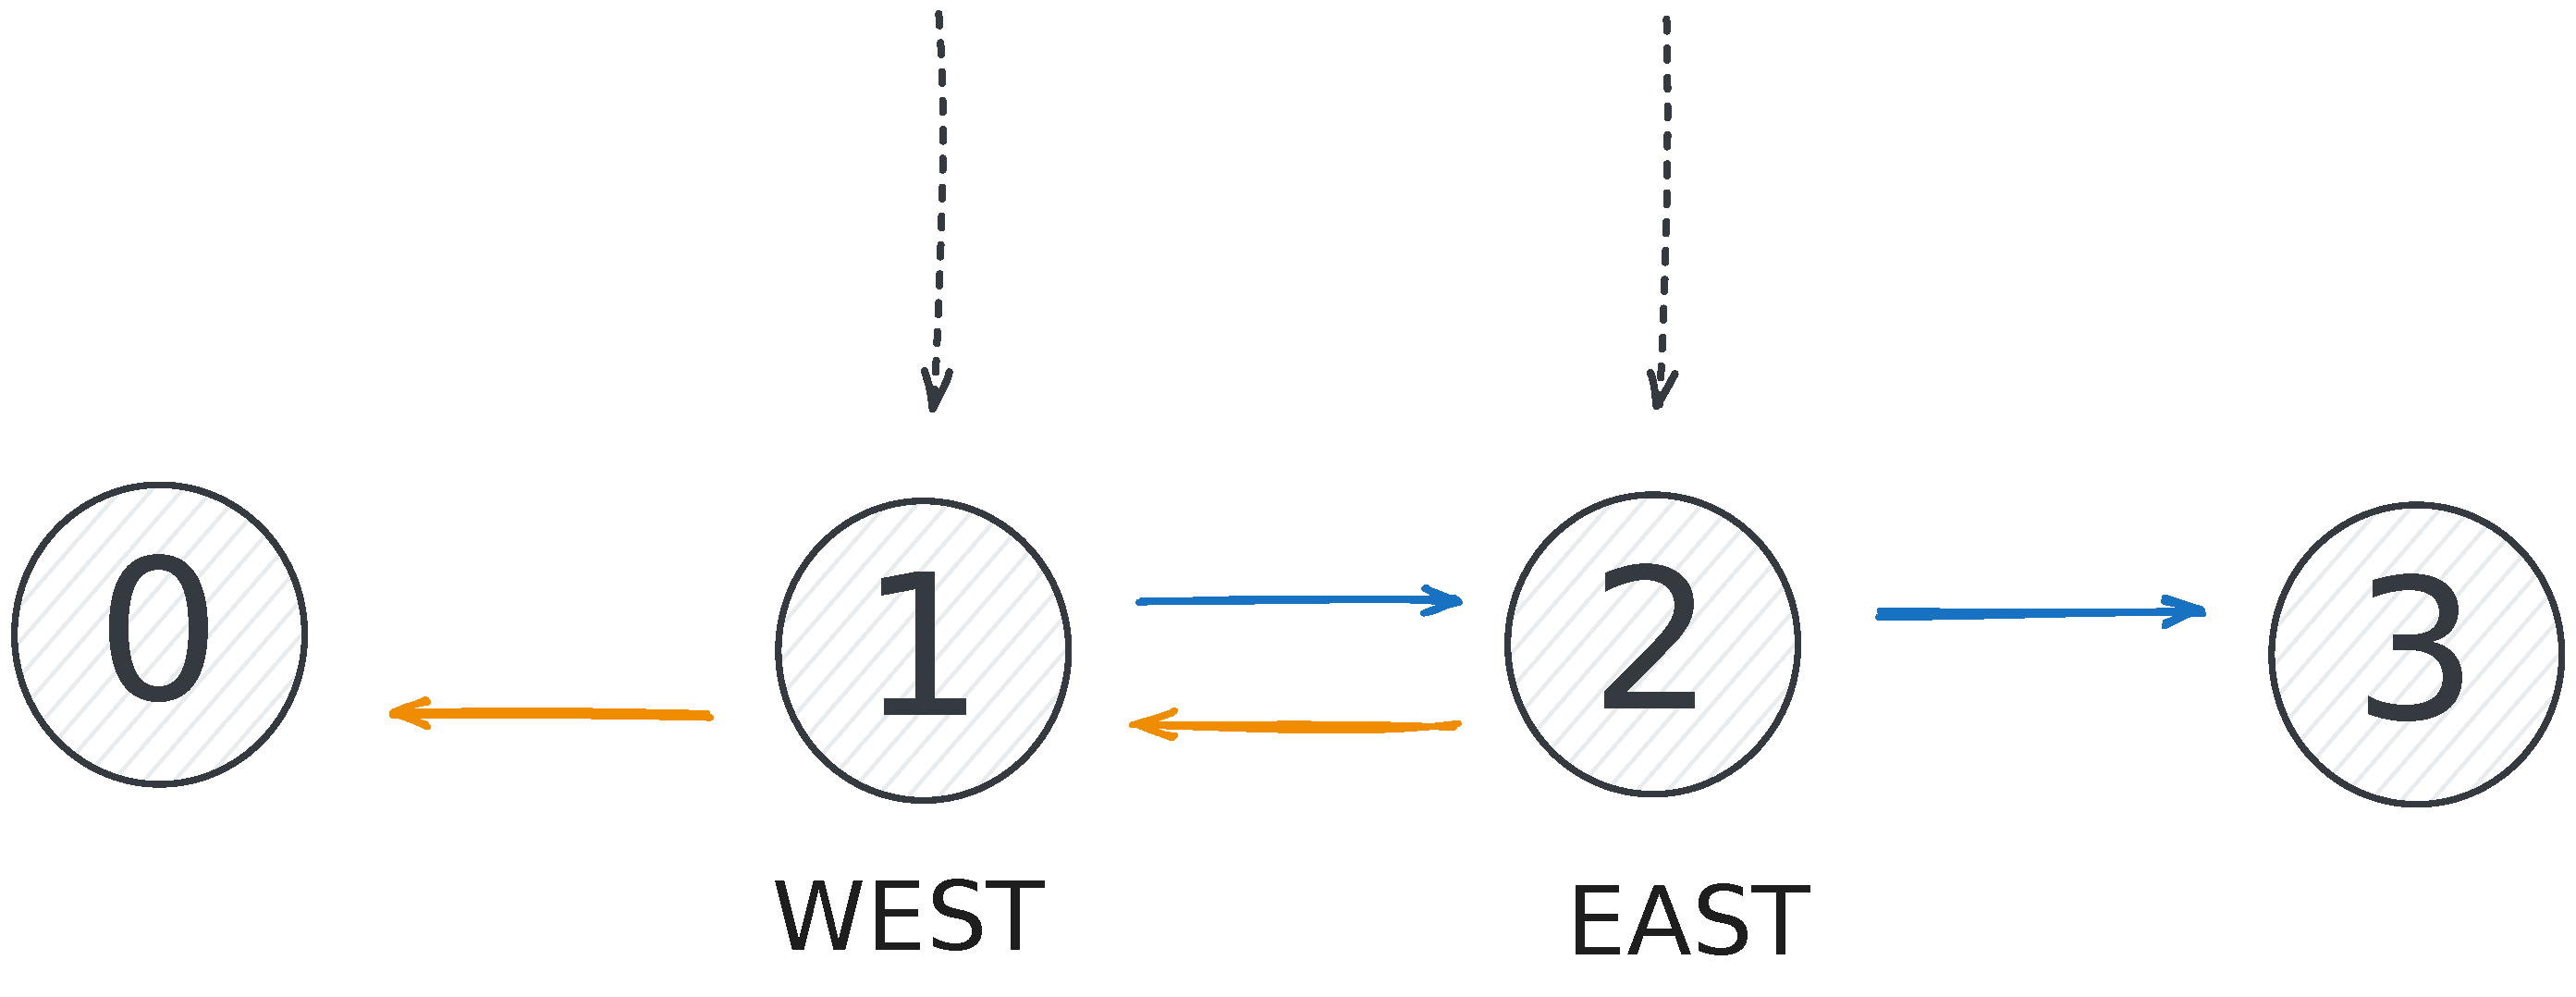
\includegraphics[
	width=\linewidth,
	trim=10 15 15 5,   % {left bottom right top} — tweak as needed
	clip
	]{plots/east_west_routing_updated_colors.pdf}
	\caption{Two routing policies.}
	\label{fig:BgpRoutingPolicies}
\end{wrapfigure}
%
%\begin{figure}[H]
%	\centering
%	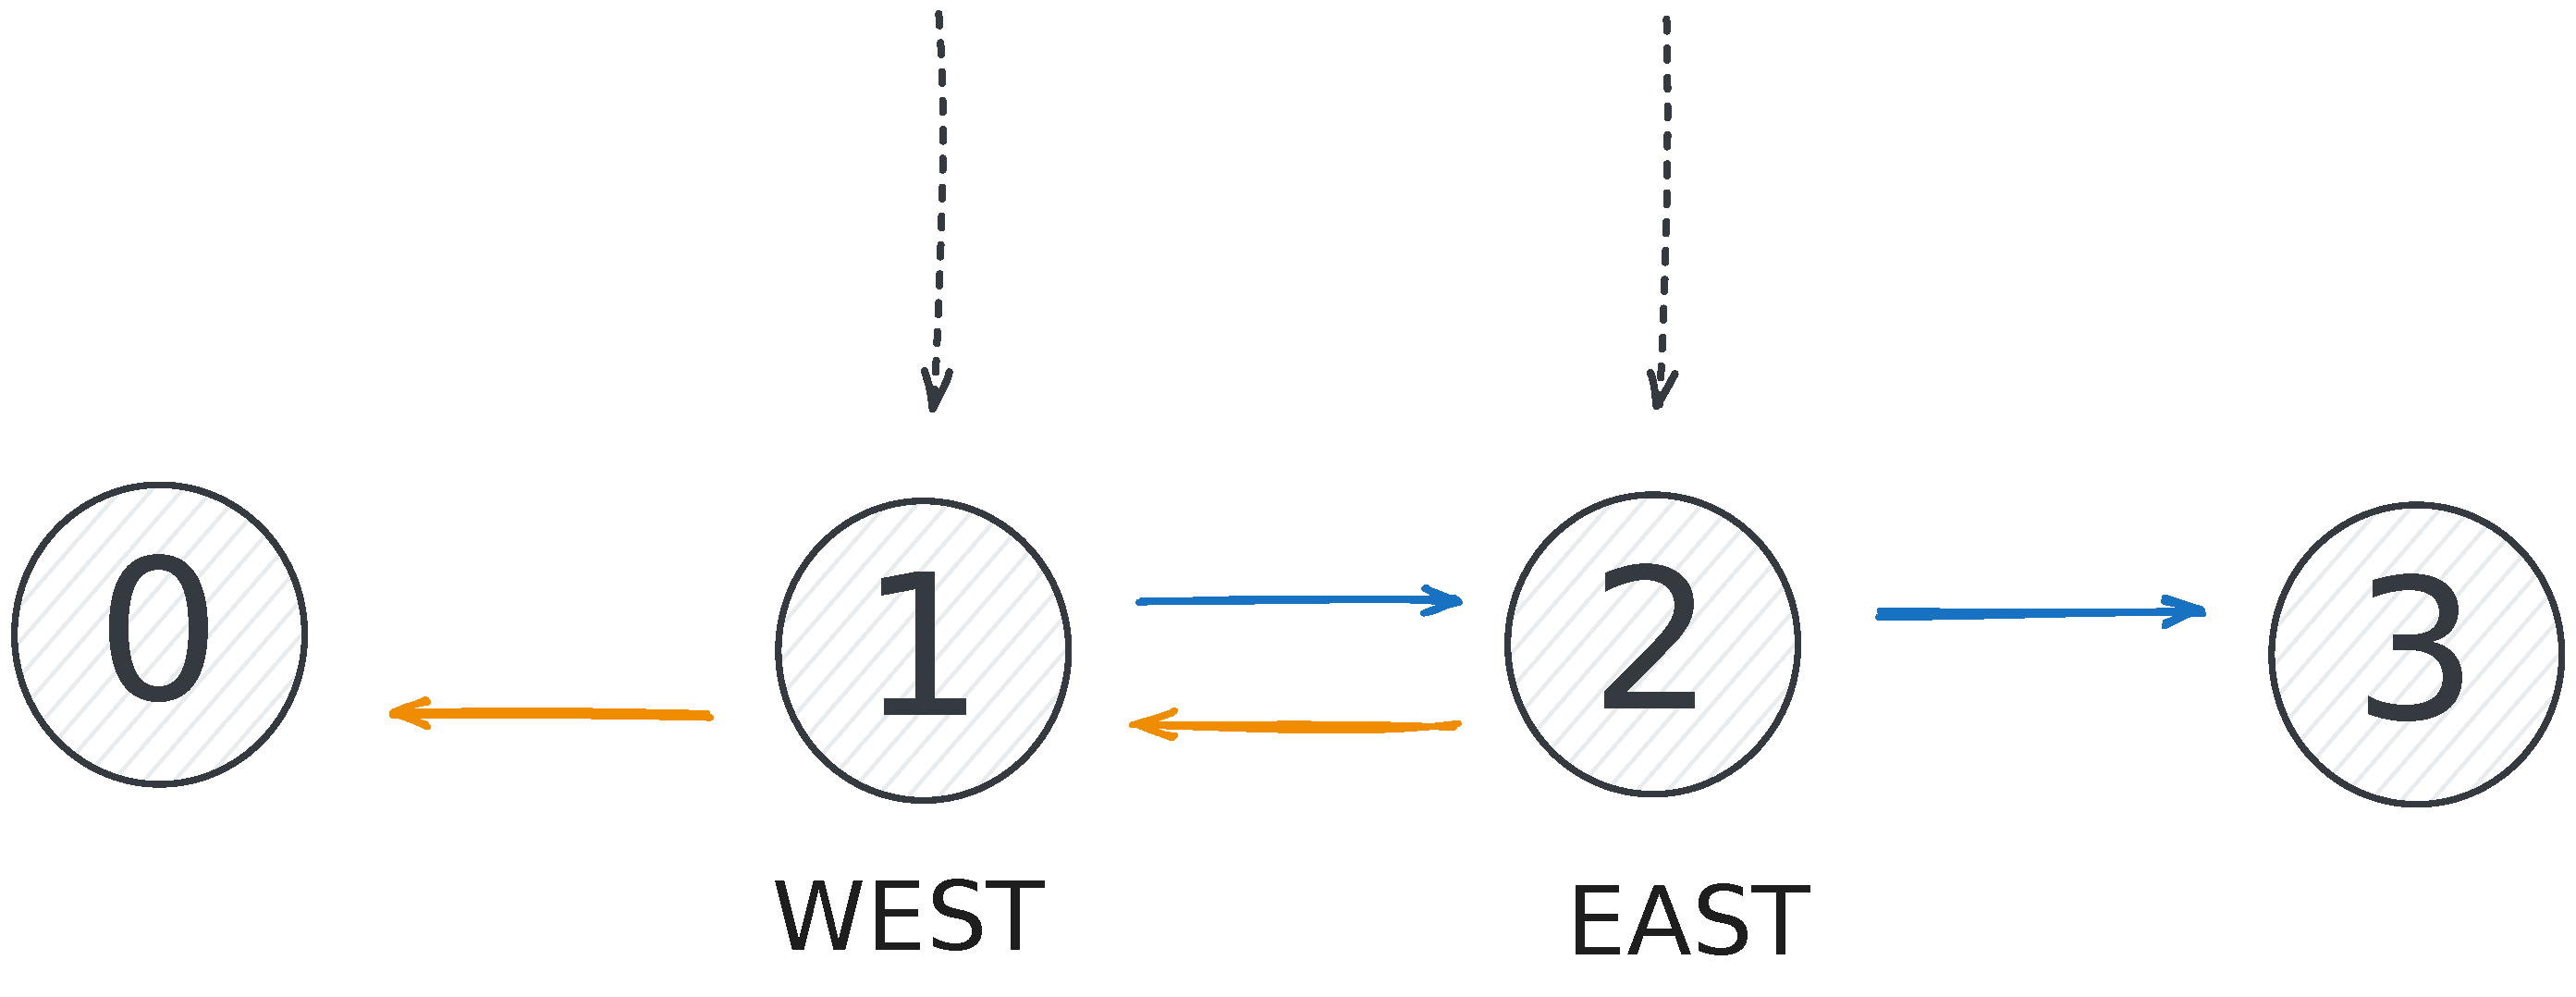
\includegraphics[width=0.5\linewidth]{plots/east_west_routing_updated_colors.pdf}
%	\caption{Routing policy in example 5.}
%	\label{fig:BgpRoutingPolicies}
%\end{figure}
%
This SDN-controlled routing policy is realized in the pseudo-code in Listing~\ref{lst:BgpNonSerializable}.
%
The program includes a single global variable \texttt{B}, indicating whether the current routing policy is \textcolor{NavyBlue}{blue} (\texttt{[B=1]}) or \textcolor{darkorange}{orange} (\texttt{[B=0]}).
%
The program has three types of requests:
%\begin{itemize}
%	
%	\item
	(i)
	{\color{ForestGreen}$\blacklozenge_\text{policy\_update}$}:
%	\textit{policy update}:
 represents a controller  update, which nondeterministically decides whether to update the policy (i.e., flip the value of  variable \texttt{B}) or not;
%	
%		\item
(ii)
	{\color{ForestGreen}$\blacklozenge_\text{route\_west}$}:
	 a request representing a packet entering the network from the \texttt{WEST} node; and 
%	
%		\item
(iii)
{\color{ForestGreen}$\blacklozenge_\text{route\_east}$}: a request representing a packet entering the network from the \texttt{EAST} node.
	%
%\end{itemize}
%
%Each of the routing requests represents a single packet entering the network. The request includes a local \textit{current} variable representing the index of the current node visited. This variable is initialized as the ingress node value, and updated to emulate the chosen routing path. There is also a \textit{visited\_east} variable (or a \textit{visited\_west} variable, depending on the request in question).
%%
%The return value of the {\color{ForestGreen}$\blacklozenge_\text{route\_from\_west}$} requests is the sum \textit{(current+current+visited\_east)}. This is an identifier encoding all possible \textit{(current\_switch, visited\_east)} pairs.
%%
%The program is not serializable, as witnessed by an interleaving that can give rise to final return value of \textit{(current+current+visited\_east)=1} (due to \textit{current=0} and \textit{visited\_east=1}). This represents a routing cycle in the network, which is possible only when updated the routing policy after a request has already been routed based on the previous policy.
%Legal, acyclic routes of this request have either a return value of 0 (in the case of [\textit{current=0}, \textit{visited\_east=0}]) or 7 (in the case of [\textit{current=3}, \textit{visited\_east=1}]).
%Potential routing cycles can also be observed via non serializable executions also for the  {\color{ForestGreen}$\blacklozenge_\text{route\_from\_east}$} requests.


\begin{center}
\begin{minipage}[!htbp]{1.0\textwidth}
	\begin{lstlisting}[caption={BGP routing (not serializable)},label={lst:BgpNonSerializable},numbers=none]
 request policy_update:
     if (?): // nondeterministically 1 or 0
         B := 1  // blue policy 
     else:
         B := 0 // orange policy
		
 request route_west:
     current := 1 // initial node
     while (current == 1) or (current == 2): // still routing        
         if (current == 1): // west (switch 1)
             if (B == 1): // blue policy
                 current := 2
             else: // orange policy
                 current := 0
         if (current == 2): // east (switch 2)
             visited_east := 1
             if (B == 1): // blue policy
                 current := 3
             else: // orange policy
                 current := 1
         yield
     return current + current + visited_east
     
 request route_east: ... // dual case      
		\end{lstlisting}
\end{minipage}
\end{center}


Each of the routing requests represents a single packet entering the network. The request includes a local \texttt{current} variable representing the index of the current node visited. This variable is initialized as the ingress node value and is updated to emulate the chosen routing path. There is also a \texttt{visited\_east} variable (or a \texttt{visited\_west} variable, depending on the request in question).
%
The return value of the {\color{ForestGreen}$\blacklozenge_\text{route\_west}$} requests is the sum \texttt{[current+current+visited\_east]}, an identifier encoding all possible \texttt{(current\_switch, visited\_east)} pairs.
%
The program is not serializable, as witnessed by an interleaving that can give rise to a final return value of \texttt{[current+current+visited\_east=1]} (due to \texttt{[current=0]} and \texttt{[visited\_east=1]}). This represents a \textit{routing cycle} in the network, which is possible only when there is an interleaving between a control packet ({\color{ForestGreen}$\blacklozenge_\text{policy\_update}$}) and a routing packet (e.g., {\color{ForestGreen}$\blacklozenge_\text{route\_west}$}). Specifically, this occurs when a request has already been spawned and began routing based on the previous policy, subsequently yields, and eventually returns after the policy was flipped based on another control packet --- hence resulting in a routing cycle.
%
More formally, this is conveyed by response values that represent these cycles and are obtained only via non-serial executions. For example, acyclic routes of this request have either a return value of 0 (in the case of [\texttt{current=0}, \texttt{visited\_east=0}]) or 7 (in the case of [\texttt{current=3}, \texttt{visited\_east=1}]).
Dually, routing cycles could also occur in the case of {\color{ForestGreen}$\blacklozenge_\text{route\_east}$} interleavings.


\subsection{Example 6}


The next program captures serializability through the lens of the \textit{snapshot isolation} consistency model, which is used in various real-world database systems, including \texttt{PostgreSQL}~\cite{postgresql-transaction-iso} and \texttt{CockroachDB}~\cite{cockroachdb-si-docs}, and has been linked to real‐world anomalies (e.g., duplicate‐key errors in the latter~\cite{cockroach-issue-14099}).
%
The depicted program has two nodes (represented by the global variables \texttt{N$_1$} and \texttt{N$_2$}) which monitor ongoing traffic in the network, and are originally both active, as indicated by their initial values: \texttt{[N$_1$=1]}, \texttt{[N$_2$=1]}.
%
The {\color{ForestGreen}$\blacklozenge_\text{main}$} request takes a snapshot of the system, i.e., locally records the current activation status of each of the two nodes.
%
Then, in the first request, and in any future ones in which both nodes are active, each in-flight request non-deterministically decides which of the two nodes to deactivate, i.e., set \texttt{[N$_i$:=0]}, for maintaining overall energy efficiency.
%
The {\color{ForestGreen}$\blacklozenge_\text{main}$} request eventually returns the current sum of active nodes in the system.
%
In order for the system to emulate multiple non-trivial interleavings, our setting also includes two additional requests, {\color{ForestGreen}$\blacklozenge_\text{activate\_n1}$} and {\color{ForestGreen}$\blacklozenge_\text{activate\_n2}$}, which activate nodes \texttt{N$_1$} and \texttt{N$_2$}, respectively.
%
We note that the program is not serializable due to the \texttt{yield} statement that appears immediately after the recorded snapshot of the node activation status. One such example of a non-serializable behavior occurs when two {\color{ForestGreen}$\blacklozenge_\text{main}$} requests are both in-flight, and each of them records two active monitor nodes and then executes \texttt{yield}; Then, each request might turn off a complement monitor node. As a result of each request operating based on its isolated snapshot of the global state, both monitor nodes can be turned off --- inducing a request with {\color{ForestGreen}$\blacklozenge_\text{main}$}/{\color{red}$\blacklozenge_0$} (for \texttt{[N$_1$+N$_2$=0+0=0]}).
%
We note that in any serial execution, no two {\color{ForestGreen}$\blacklozenge_\text{main}$} requests can \textit{simultaneously} record both monitors as active, and hence, a response of {\color{red}$\blacklozenge_0$} cannot be obtained by serial executions.




\begin{minipage}[htbp]{1.1\textwidth}
	\begin{lstlisting}[caption={Snapshot-based monitor deactivation (not serializable)},numbers=none]
// initialize both monitors to be active
N_1_ACTIVE := 1
N_2_ACTIVE := 1

request main:
    // take snapshot
    n_1_active_snapshot := N_1_ACTIVE
    n_2_active_snapshot := N_2_ACTIVE
    yield

    if (n_1_active_snapshot == 1) and (n_2_active_snapshot == 1):
        // if both nodes active --- choose which one to deactivate 
        if (?): 
            N_1_ACTIVE := 0
        else:
            N_2_ACTIVE := 0

    return N_1_ACTIVE + N_2_ACTIVE  // total active nodes


request activate_n1:
    N_1_ACTIVE := 1

request activate_n2:
    N_2_ACTIVE := 1
		
		
	\end{lstlisting}
\end{minipage}


%We include an additional network‐monitoring example under \textit{snapshot isolation} in Appendix~\ref{appendix:snapshotIsolationExample}. Snapshot isolation is supported by production databases such as \texttt{PostgreSQL}~\cite{postgresql-transaction-iso} and \texttt{CockroachDB}~\cite{cockroachdb-si-docs}, and has been linked to real‐world anomalies (e.g., duplicate‐key errors in the latter~\cite{cockroach-issue-14099}).

%We add an additional example for network monitoring and \textit{snapshot isolation} in Appendix~\ref{appendix:snapshotIsolationExample}. Snapshot isolation is a consistency model used in production systems such as \texttt{PostgreSQL}~\cite{postgresql-transaction-iso} and \texttt{CockroachDB}~\cite{cockroachdb-si-docs}, and has been implicated in real-world bugs (e.g.,see the report on duplicate key errors ins \texttt{CockroachDB}~\cite{cockroach-issue-14099}).


%We add an additional example for network monitoring and \textit{snapshot isolation} in Appendix~\ref{appendix:snapshotIsolationExample}.%, and its relation to serializability.
%\guy{suddenly I'm not so sure about this example. It is indeed sound but maybe a bit silly?}




\section{SER Small-Step Semantics}
\label{appendix:ser-semantics}

%
%\subsection{Semantics}
%
The set \(\texttt{V}\) is a finite set of numeric constants; booleans use $0/1$. We respectively denote with \(\texttt{VARS}\) and \(\texttt{vars}\) the (finite) sets of global and local variables. Mappings $\rho:{\texttt{vars}}\to \texttt{V}$ and $g:{\texttt{VARS}}\to \texttt{V}$ respectively map a local or global variable to its current value in \(\texttt{V}\).
%
Configurations are denoted as $\cfg{e}{\rho}{g}$, with \(e\) being a valid \toolname{} expression. 
%
Small steps are denoted $(\step)$, while big steps are denoted $(\pstep)$, and may comprise of a sequence of small steps (also denoted $\step^{*}$).
%
%program configurations $\langle g , \Pi\rangle$ with \(g\) being a global state and \(\Pi\) being set of in-flight \((e,\ell)\) pairs.
%
%We denote with \(\ell_0\) the initial local state of every packet.

\smallskip
\noindent\textit{Small step} $(\step)$.
\begin{mathpar}
	\inferrule*[right=ND-0]{ }{\cfg{\nondet}{\rho}{g} \step \cfg{0}{\rho}{g}}
	\and
	\inferrule*[right=ND-1]{ }{\cfg{\nondet}{\rho}{g} \step \cfg{1}{\rho}{g}}\\
	
	\inferrule*[right=LOCAL-READ]{\rho(x)=v\quad v\in{\texttt{V}}}{\cfg{x}{\rho}{g} \step \cfg{v}{\rho}{g}}
	\and
	\inferrule*[right=GLOBAL-READ]{g(X)=v \quad v\in{\texttt{V}}}{\cfg{X}{\rho}{g} \step \cfg{v}{\rho}{g}}\\
	
	\inferrule*[right=LOCAL-WRITE-STEP]{\cfg{e}{\rho}{g} \step \cfg{e'}{\rho'}{g'}}{\cfg{x := e}{\rho}{g} \step \cfg{x := e'}{\rho'}{g'}}
	\and
	\inferrule*[right=LOCAL-WRITE-DONE]{v\in{\texttt{V}}}{\cfg{x := v}{\rho}{g} \step \cfg{v}{\update{\rho}{x}{v}}{g}}
	
	\inferrule*[right=GLOBAL-WRITE-STEP]{\cfg{e}{\rho}{g} \step \cfg{e'}{\rho'}{g'}}{\cfg{X := e}{\rho}{g} \step \cfg{X := e'}{\rho'}{g'}}
	\and
	\inferrule*[right=GLOBAL-WRITE-DONE]{v\in{\texttt{V}}}{\cfg{X := v}{\rho}{g} \step \cfg{v}{\rho}{\update{g}{X}{v}}}
	
	\inferrule*[right=EQ-L]{\cfg{e_1}{\rho}{g} \step \cfg{e_1'}{\rho'}{g'}}{\cfg{e_1 == e_2}{\rho}{g} \step \cfg{e_1' == e_2}{\rho'}{g'}}
	\and
	\inferrule*[right=EQ-R]{\cfg{e_2}{\rho}{g} \step \cfg{e_2'}{\rho'}{g'}}{\cfg{v_1 == e_2}{\rho}{g} \step \cfg{v_1 == e_2'}{\rho'}{g'}}
	\and
	\inferrule*[right=EQ-T]{v_1=v_2\quad v_1, v_2\in{\texttt{V}}}{\cfg{v_1 == v_2}{\rho}{g} \step \cfg{1}{\rho}{g}}
	\and
	\inferrule*[right=EQ-F]{v_1\neq v_2 \quad v_1, v_2\in{\texttt{V}}}{\cfg{v_1 == v_2}{\rho}{g} \step \cfg{0}{\rho}{g}}
	\end{mathpar}
	
	\begin{mathpar}
	\inferrule*[right=SEQ-STEP]{\cfg{e_1}{\rho}{g} \step \cfg{e_1'}{\rho'}{g'}}{\cfg{e_1 ; e_2}{\rho}{g} \step \cfg{e_1' ; e_2}{\rho'}{g'}}
	\and
	\inferrule*[right=SEQ-DONE]{v\in{\texttt{V}}}{\cfg{v ; e_2}{\rho}{g} \step \cfg{e_2}{\rho}{g}}

	\inferrule*[right=IF-GUARD]{\cfg{e_1}{\rho}{g} \step \cfg{e_1'}{\rho'}{g'}}{\cfg{\ifkw(e_1)\{e_2\}\elsekw\{e_3\}}{\rho}{g} \step \cfg{\ifkw(e_1')\{e_2\}\elsekw\{e_3\}}{\rho'}{g'}}
	\and
	\inferrule*[right=IF-T]{ }{\cfg{\ifkw(1)\{e_2\}\elsekw\{e_3\}}{\rho}{g} \step \cfg{e_2}{\rho}{g}}
	\and
	\inferrule*[right=IF-F]{ }{\cfg{\ifkw(0)\{e_2\}\elsekw\{e_3\}}{\rho}{g} \step \cfg{e_3}{\rho}{g}}
	
	\inferrule*[right=WHILE-UNFOLD]{ }{\cfg{\whilekw(e_1)\{e_2\}}{\rho}{g}
		\step
		\cfg{\ifkw(e_1)\{\,e_2 ; \whilekw(e_1)\{e_2\}\,\}\elsekw\{0\}}{\rho}{g}}
\end{mathpar}

\noindent\textit{Big step} $(\pstep)$ and scheduling.
\begin{mathpar}
	\inferrule*[right=YIELD]{\cfg{e}{\rho}{g} \step^{*} \cfg{\yieldkw ; e'}{\rho'}{g'}}{\cfg{e}{\rho}{g} \pstep \cfg{e'}{\rho'}{g'}}
	\\
%	\inferrule*[right=START]{\cfg{e_i}{\rho}{g}\pstep \cfg{e'_i}{\rho'}{g'} \quad name_i\{e_i\}\in P_0}{\langle \requestkw\ name_i\{e_i\}, \rho, g \rangle \pstep  \cfg{e'_i}{\rho'}{g'} }
%	\and
	\inferrule*[right=TERMINATE]{\cfg{e}{\rho}{g} \step^{*} \cfg{v}{\rho'}{g'} \quad v\in{\texttt{V}}}{\cfg{e}{\rho}{g} \pstep \cfg{v}{\rho'}{g'}}	
\end{mathpar}



\smallskip
\noindent
\textbf{Note.}
Instead of defining a \texttt{spawn} instruction, as exists in some languages --- \toolname{} captures \textit{external} spawning via requests.
%
This setting can equivalently capture self-spawning (by using additional global variables), while translating more naturally to the networking domain --- in which threads are captured by packets sent by an external user.


\section{Additional NS Examples}
\label{appendix:MoreNsExamples}


%\subsection{Motivating Examples --- Explanation}
%
%
%Observe the simple program depicted in Listing~\ref{lst:MotivatingExample1Ser}. Each  {\color{ForestGreen}$\blacklozenge_\text{main}$} gives rise to a fresh in-flight request. The variable ``X'' is global, and shared among all in-flight requests, while the variable ``y'' is a local variable, per each request. 
%%
%As there are no yields, it is straightforward to see that the program is trivially serializable, with every request {\color{ForestGreen}$\blacklozenge_\text{main}$}: (i) assigning 1 to the global variable X; (ii) assigning y the value of X, i.e., always 1; (iii) assigning X the value 0; and (iv) returning the response y ({\color{red}$\blacklozenge_1$}). This results to every request/response pair to be of the form {\color{ForestGreen}$\blacklozenge_\text{main}$}/{\color{red}$\blacklozenge_1$}.
%%
%The program is slightly altered (in Listing~\ref{lst:MotivatingExample2NonSer}), by adding a yield operation between the aforementioned steps (i) and (ii). Now, by running two {\color{ForestGreen}$\blacklozenge_\text{main}$} requests that interleave, it is possible to attain a {\color{ForestGreen}$\blacklozenge_\text{main}$}/{\color{red}$\blacklozenge_0$} request/response pair, which is unattainable in any serial execution of Listing~\ref{lst:MotivatingExample2NonSer} --- as any such serial execution is equivalent to Listing~\ref{lst:MotivatingExample1Ser}, which always responds {\color{red}$\blacklozenge_1$} to any request {\color{ForestGreen}$\blacklozenge_\text{main}$}.
%%
%The program is altered once again in in Listing~\ref{lst:MotivatingExample3Ser}, by adding a fresh global variable ``L'', indicating whether the critical section is locked ($L=1$) or not ($L=0$).
%By adding a global lock variable, even if an interleaving occurs after yielding, the lock will allow only the first request to terminate, and will then release the lock for the next request. Hence, despite having yields, we attain serializable executions, and only {\color{ForestGreen}$\blacklozenge_\text{main}$}/{\color{red}$\blacklozenge_1$} request/response pairs are produced, similar to the original program in Listing~\ref{lst:MotivatingExample1Ser}.
%%
%This simple example demonstrates the motivation for automatic serializability checking, as even small, toy programs can be surprisingly difficult to reason about when assessing their serializable behavior.
%





\subsection{Motivating Example \#1}
\label{appendix:subsec::Ex1A:NS}


For our first motivating example, presented in Listing~\ref{lst:MotivatingExample1Ser}, we present the Network System in Fig.~\ref{fig:code1ExampleNS}, the Serialized NFA in Fig.~\ref{fig:code1ExampleNFA}, and the Interleaving Petri Net in Fig.~\ref{fig:code1ExamplePN}.


%\begin{minipage}[t]{0.3\textwidth}
%	\begin{lstlisting}[caption={Without yield or lock (serializable)}]
%	request main: 
%		X := 1 
%		// no yield
%		y := X 
%		X := 0
%		return y 
%	\end{lstlisting}
%\end{minipage}

\begin{figure}[!htbp]
	\centering
	% \includegraphics[width=\textwidth]{plots/code_single_path_NS.png}\\[1ex]
	
	\begin{tikzpicture}[
		node distance=1.5cm and 2.5cm,
		>=stealth,
		thick,
		every node/.style={font=\small}
		]
		%––– Request (main) –––
		\node[
		draw=black,
		line width=0.8pt,
		fill=ForestGreen!20,
		text=black,
		diamond,
		aspect=2,
		inner sep=2pt,
		scale=0.7
		] (main) {\texttt{main}};
		
		%––– First state: y=0 + full program –––
		\node[right=0.7cm of main, align=center] (state1) {
			\begin{tikzpicture}[baseline=(ybox.base)]
				\node[
				draw=black,
				line width=0.8pt,
				fill=brightyellow,
				text=black,
				rectangle,
				rounded corners=1pt,
				inner sep=2pt
				] (ybox) {\texttt{y=0}};
			\end{tikzpicture}\\[-2.5pt]
			\begin{minipage}{2cm}
				\begin{lstlisting}[language=CustomPseudoCode,numbers=none,basicstyle=\tiny\ttfamily]
X := 1
// no yield
y := X
X := 0
return y
				\end{lstlisting}
			\end{minipage}
		};
		
		%––– Second state: y=1 + //end –––
		\node[right=of state1, align=center] (state2) {
			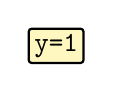
\begin{tikzpicture}[baseline=(ybox.base)]
				\node[
				draw=black,
				line width=0.8pt,
				fill=brightyellow,
				text=black,
				rectangle,
				rounded corners=1pt,
				inner sep=2pt
				] (ybox) {\texttt{y=1}};
			\end{tikzpicture}\\[-2.5pt]
			\begin{minipage}{0.8cm}
				\begin{lstlisting}[language=CustomPseudoCode,numbers=none,basicstyle=\tiny\ttfamily]
// end
				\end{lstlisting}
			\end{minipage}
		};
		
		%––– Response "1" –––
		\node[
		right=0.6cm of state2,
		draw=black,
		line width=0.8pt,
		fill=RedViolet!20,
		text=black,
		diamond,
		aspect=2,
		inner sep=2pt,
		scale=0.7,
		font=\Large
		] (resp1) {\texttt{1}};
		
		%––– Arrows –––
		\draw[->] (main) -- (state1);
		
		% Single transition label: X=0 -> X=1
		\draw[->] (state1) -- node[above] {%
			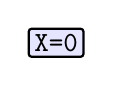
\begin{tikzpicture}[baseline=(a.base)]
				\node[draw=black,line width=0.8pt,fill=blue!10,rectangle,rounded corners=1pt,inner sep=2pt] (a) {\texttt{X=0}};
			\end{tikzpicture}
			$\to$
			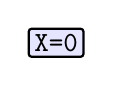
\begin{tikzpicture}[baseline=(b.base)]
				\node[draw=black,line width=0.8pt,fill=blue!10,rectangle,rounded corners=1pt,inner sep=2pt] (b) {\texttt{X=0}};
			\end{tikzpicture}
		} (state2);
		
		% To response "1"
		\draw[->] (state2) -- (resp1);
		
	\end{tikzpicture}
	
	\caption{Network System for interleaving executions of the program in Listing~\ref{lst:MotivatingExample1Ser}.}
\label{fig:code1ExampleNS}
\end{figure}



%\begin{figure}[!htbp]
%	\centering
%	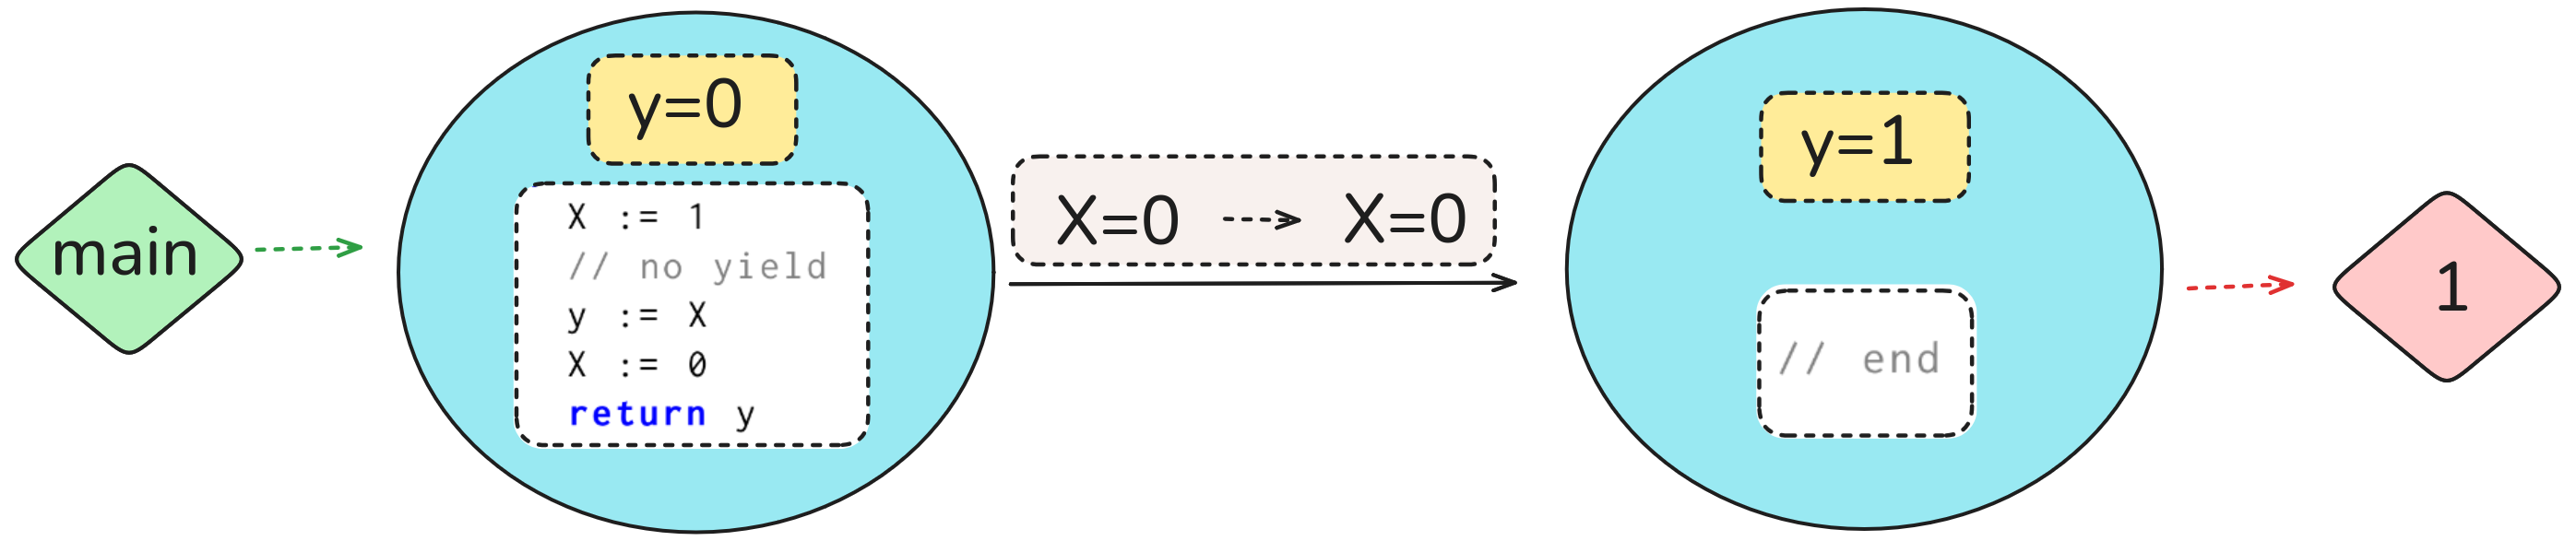
\includegraphics[width=0.9\textwidth]{plots/code_1_NS.png}
%	\caption{Network System for interleaving executions of the program in Listing~\ref{lst:MotivatingExample1Ser}.}
%	\label{fig:code1ExampleNS}
%\end{figure}


%\begin{figure}[!htbp]
%	\centering
%	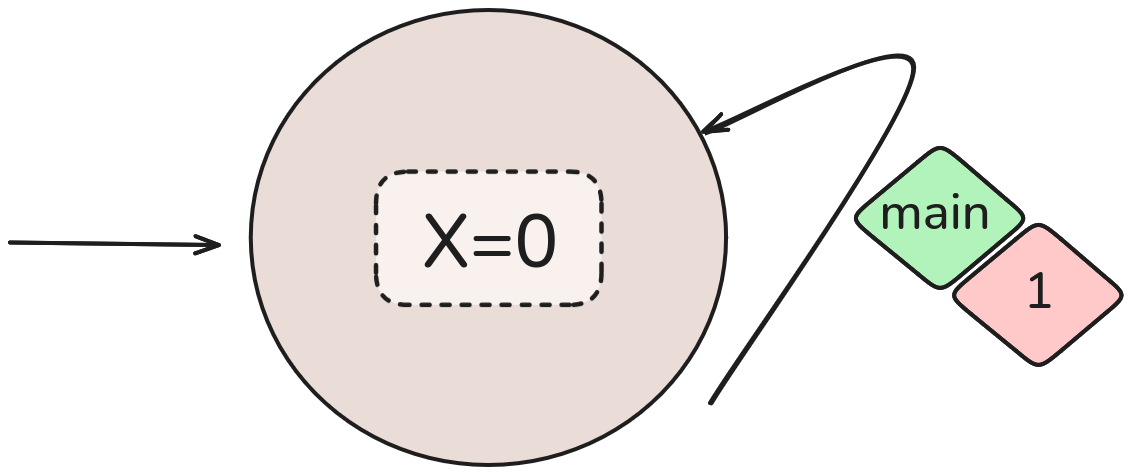
\includegraphics[width=0.35\textwidth]{plots/code_1_NFA.png}
%	\caption{NFA for serial executions of the program in Listing~\ref{lst:MotivatingExample1Ser}.}
%	\label{fig:code1ExampleNFA}
%\end{figure}


\begin{figure}  [!htbp]
	\centering
	% \includegraphics[width=0.48\textwidth,trim=0 0 0 0,clip]{plots/code_single_X0_NFA.pdf}
	
	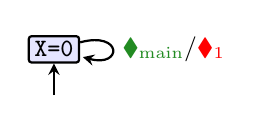
\begin{tikzpicture}[
		->,>=stealth,
		thick,
		node distance=2.5cm,
		state/.style={
			draw=black,
			line width=0.8pt,
			fill=blue!10,
			rectangle,
			rounded corners=1pt,
			inner sep=2pt,
			font=\small
		},
		every node/.style={font=\small}
		]
		% Single state
		\node[state] (X0) {\texttt{X=0}};
		
		% Initial state arrow
		\draw[->] ([yshift=-0.4cm]X0.south) -- (X0.south);
		
		% Self-loop with main/1 using the paper's colored lozenge notation
		\draw[->] (X0) edge[loop right]
		node[right] {${\color{ForestGreen}\blacklozenge_{\mathrm{main}}}/{\color{red}\blacklozenge_1}$} (X0);
	\end{tikzpicture}
	
	\caption{NFA for serial executions of the program in Listing~\ref{lst:MotivatingExample1Ser}.}
\label{fig:code1ExampleNFA}
\end{figure}




\begin{figure}[H]
	\centering
	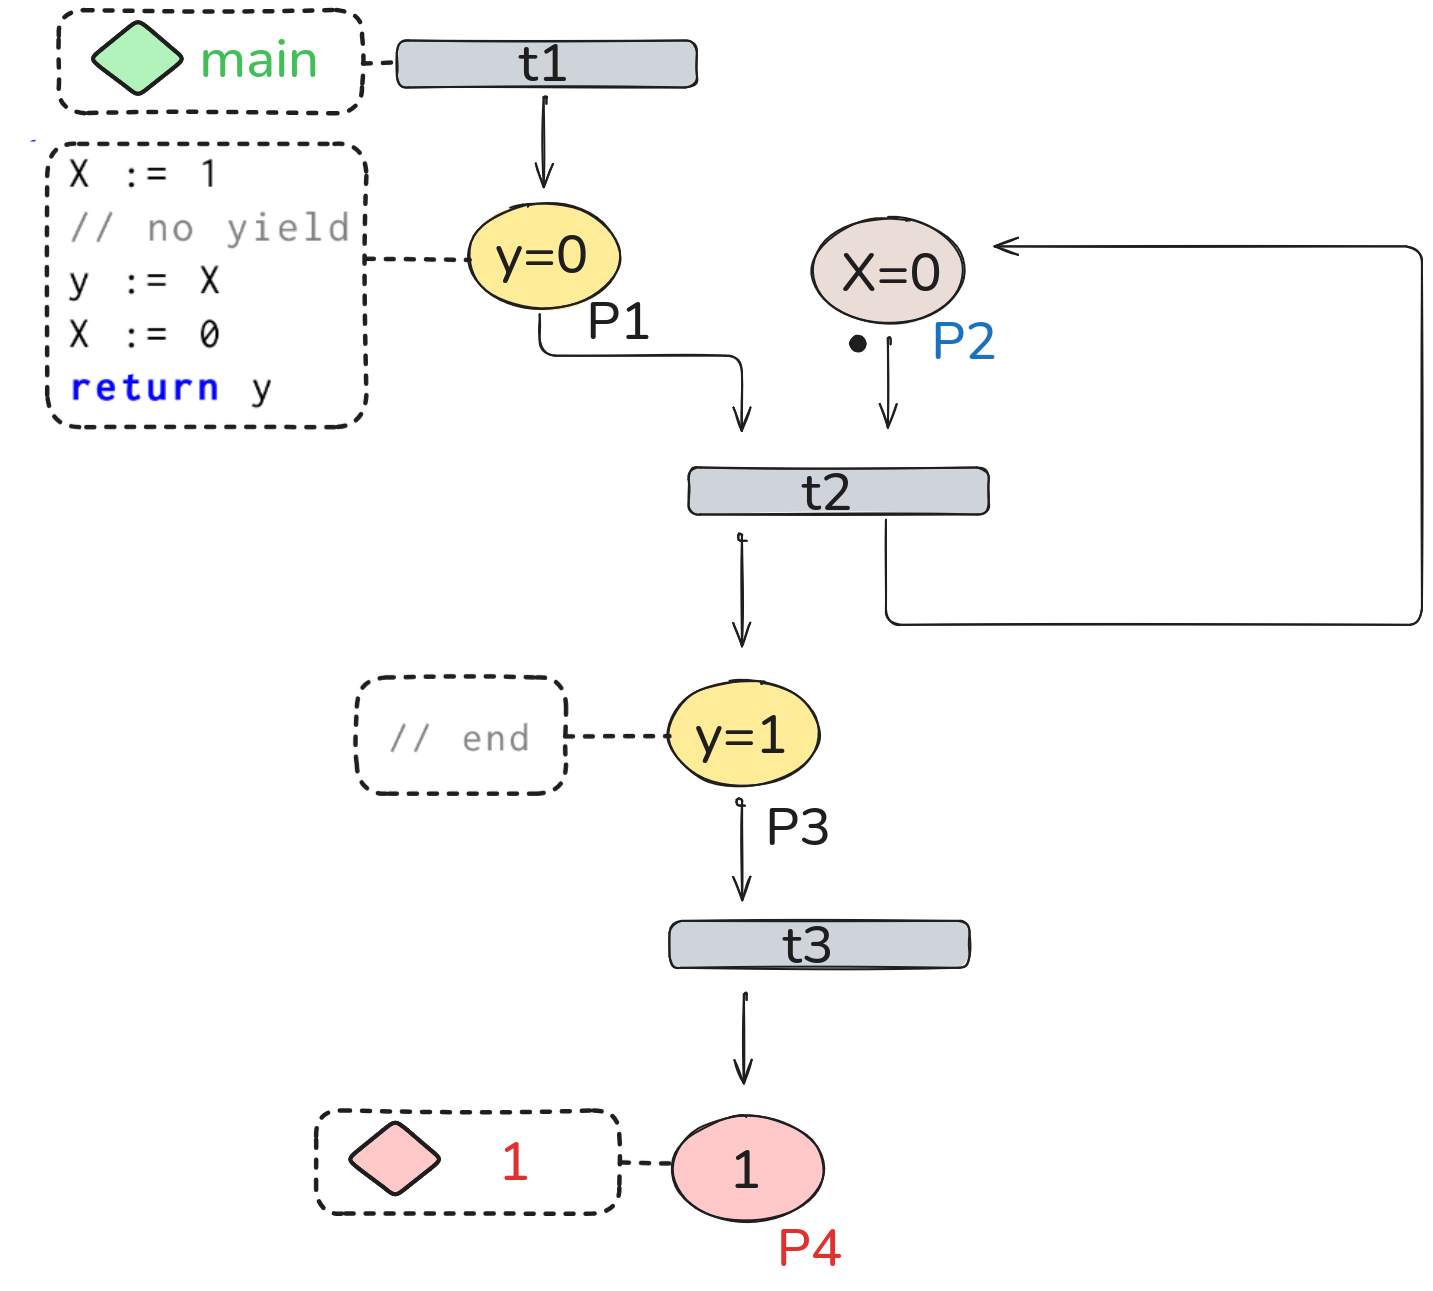
\includegraphics[width=0.6\textwidth]{plots/code_1_PN_with_annotation.png}
	\caption{Petri Net for interleaving executions of the program in Listing~\ref{lst:MotivatingExample1Ser}.}
	\label{fig:code1ExamplePN}
\end{figure}


%

\subsection{Motivating Examples \#2}
\label{appendix:subsec::Ex1B:NS}

For details, see the main text (Sec.~\ref{sec:problem-definition}).


\subsection{Motivating Examples \#3}
\label{appendix:subsec:Ex1C:NS}


For our third motivating example, presented in Listing~\ref{lst:MotivatingExample3Ser}, we present the Network System in Fig.~\ref{fig:code3ExampleNS}, the Serialized NFA in Fig.~\ref{fig:code3ExampleNFA}, and the Interleaving Petri Net in Fig.~\ref{fig:code3ExamplePN}

%\begin{minipage}[t]{0.3\textwidth}
%	\begin{lstlisting}[caption={With yield and lock (serializable)}]
%		request foo: 
%			// lock
%			while (L == 1): 
%				yield
%			L := 1 
%		
%			X := 1
%			yield
%			y := X 
%			X := 0
%		
%			// unlock    
%			L := 0
%			return y 
%	\end{lstlisting}
%\end{minipage}
%
%This program corresponds to the following Network System (NS):

%\begin{figure}[!htbp]
%	\centering
%	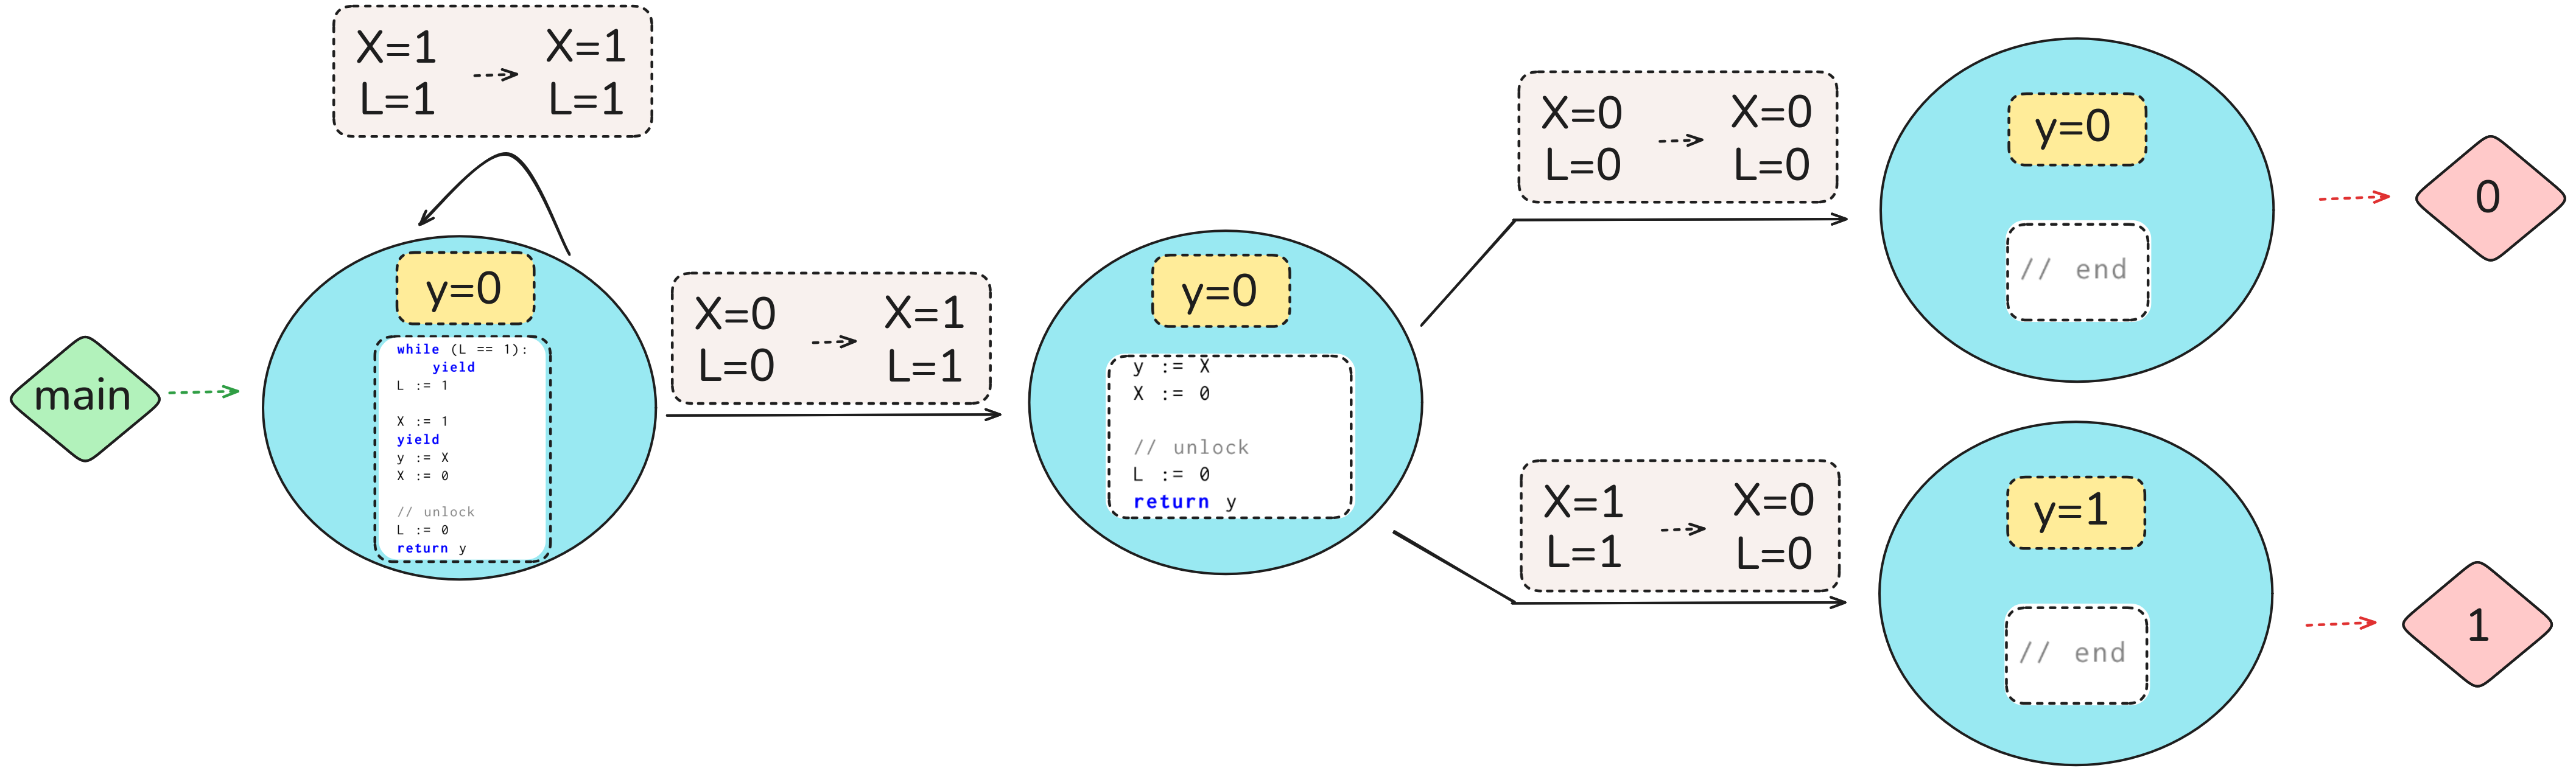
\includegraphics[width=1.1\textwidth]{plots/code_3_NS.png}
%	\caption{Network System for interleaving executions of the program in Listing~\ref{lst:MotivatingExample3Ser}.}
%	\label{fig:code3ExampleNS}
%\end{figure}


\begin{figure}[!htbp]
	\centering
	% \includegraphics[width=\textwidth]{plots/code_locking_NS.png}\\[1ex]
	
	\begin{tikzpicture}[
		node distance=1.5cm and 2.5cm,
		>=stealth,
		thick,
		every node/.style={font=\small}
		]
		%–––– Request (green diamond) ––––
		\node[
		draw=black,
		line width=0.8pt,
		fill=ForestGreen!20,
		text=black,
		diamond,
		aspect=2,
		inner sep=2pt,
		scale=0.7
		] (main) {\texttt{main}};
		
		%–––– State 1: y=0 + locked program ––––
		\node[right=0.7cm of main, align=center] (state1) {
			\begin{tikzpicture}[baseline=(ybox.base)]
				\node[
				draw=black,
				line width=0.8pt,
				fill=brightyellow,
				text=black,
				rectangle,
				rounded corners=1pt,
				inner sep=2pt
				] (ybox) {\texttt{y=0}};
			\end{tikzpicture}\\[-2.5pt]
			\begin{minipage}{2.6cm}
				\begin{lstlisting}[language=CustomPseudoCode,numbers=none,basicstyle=\tiny\ttfamily]
while (L == 1):
	yield
L := 1

X := 1
yield
y := X
X := 0

// unlock
L := 0
return y
				\end{lstlisting}
			\end{minipage}
		};
		
		%–––– State 2: y=0 + tail program ––––
		\node[right=of state1, xshift=12mm, align=center] (state2) {
			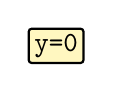
\begin{tikzpicture}[baseline=(ybox.base)]
				\node[
				draw=black,
				line width=0.8pt,
				fill=brightyellow,
				text=black,
				rectangle,
				rounded corners=1pt,
				inner sep=2pt
				] (ybox) {\texttt{y=0}};
			\end{tikzpicture}\\[-2.5pt]
			\begin{minipage}{2.0cm}
				\begin{lstlisting}[language=CustomPseudoCode,numbers=none,basicstyle=\tiny\ttfamily]
y := X
X := 0

// unlock
L := 0
return y
				\end{lstlisting}
			\end{minipage}
		};
		
		%–––– State 3 (top-right): //end, y=0 ––––
		\node[above right=-0.5cm and 2.2cm of state2, align=center] (state3) {
			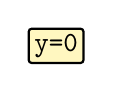
\begin{tikzpicture}[baseline=(ybox.base)]
				\node[
				draw=black,
				line width=0.8pt,
				fill=brightyellow,
				text=black,
				rectangle,
				rounded corners=1pt,
				inner sep=2pt
				] (ybox) {\texttt{y=0}};
			\end{tikzpicture}\\[-2.5pt]
			\begin{minipage}{0.9cm}
				\begin{lstlisting}[language=CustomPseudoCode,numbers=none,basicstyle=\tiny\ttfamily]
// end
				\end{lstlisting}
			\end{minipage}
		};
		
		%–––– State 4 (bottom-right): //end, y=1 ––––
		\node[below right=-0.2cm and 2.2cm of state2, align=center] (state4) {
			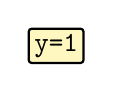
\begin{tikzpicture}[baseline=(ybox.base)]
				\node[
				draw=black,
				line width=0.8pt,
				fill=brightyellow,
				text=black,
				rectangle,
				rounded corners=1pt,
				inner sep=2pt
				] (ybox) {\texttt{y=1}};
			\end{tikzpicture}\\[-2.5pt]
			\begin{minipage}{0.9cm}
				\begin{lstlisting}[language=CustomPseudoCode,numbers=none,basicstyle=\tiny\ttfamily]
// end
				\end{lstlisting}
			\end{minipage}
		};
		
		%–––– Responses ––––
		\node[
		right=0.6cm of state3,
		draw=black,
		line width=0.8pt,
		fill=RedViolet!20,
		text=black,
		diamond,
		aspect=2,
		inner sep=2pt,
		scale=0.7,
		font=\Large
		] (resp0) {\texttt{0}};
		
		\node[
		right=0.6cm of state4,
		draw=black,
		line width=0.8pt,
		fill=RedViolet!20,
		text=black,
		diamond,
		aspect=2,
		inner sep=2pt,
		scale=0.7,
		font=\Large
		] (resp1) {\texttt{1}};
		
		%–––– Arrows ––––
		\draw[->] (main) -- (state1);
		
		% Self-loop on state1: (X=1,L=1) -> (X=1,L=1)
		\draw[->] (state1) edge[loop above]
		node[above] {%
			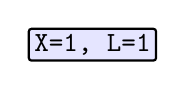
\begin{tikzpicture}[baseline=(a.base)]
				\node[draw=black,line width=0.8pt,fill=blue!10,rectangle,rounded corners=1pt,inner sep=2pt] (a) {\texttt{X=1, L=1}};
			\end{tikzpicture}
			$\to$
			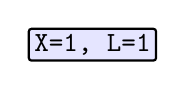
\begin{tikzpicture}[baseline=(b.base)]
				\node[draw=black,line width=0.8pt,fill=blue!10,rectangle,rounded corners=1pt,inner sep=2pt] (b) {\texttt{X=1, L=1}};
			\end{tikzpicture}
		} (state1);
		
		% Transition state1 -> state2: (X=0,L=0) -> (X=1,L=1)
		\draw[->] (state1) -- node[above] {%
			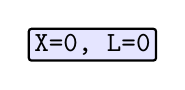
\begin{tikzpicture}[baseline=(a.base)]
				\node[draw=black,line width=0.8pt,fill=blue!10,rectangle,rounded corners=1pt,inner sep=2pt] (a) {\texttt{X=0, L=0}};
			\end{tikzpicture}
			$\to$
			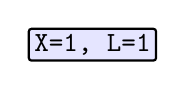
\begin{tikzpicture}[baseline=(b.base)]
				\node[draw=black,line width=0.8pt,fill=blue!10,rectangle,rounded corners=1pt,inner sep=2pt] (b) {\texttt{X=1, L=1}};
			\end{tikzpicture}
		} (state2);
		
		% Transition state2 -> state3: (X=0,L=0) -> (X=0,L=0)
		\draw[->] ([yshift=4pt]state2.east) to[out=50,in=180]
		node[above,sloped] {%
			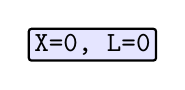
\begin{tikzpicture}[baseline=(a.base)]
				\node[draw=black,line width=0.8pt,fill=blue!10,rectangle,rounded corners=1pt,inner sep=2pt] (a) {\texttt{X=0, L=0}};
			\end{tikzpicture}
			$\to$
			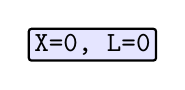
\begin{tikzpicture}[baseline=(b.base)]
				\node[draw=black,line width=0.8pt,fill=blue!10,rectangle,rounded corners=1pt,inner sep=2pt] (b) {\texttt{X=0, L=0}};
			\end{tikzpicture}
		} (state3.west);
		
		% Transition state2 -> state4: (X=1,L=1) -> (X=0,L=0)
		\draw[->] ([yshift=-16pt]state2.east) to[out=-50,in=180]
		node[below,sloped] {%
			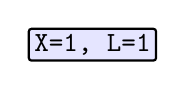
\begin{tikzpicture}[baseline=(a.base)]
				\node[draw=black,line width=0.8pt,fill=blue!10,rectangle,rounded corners=1pt,inner sep=2pt] (a) {\texttt{X=1, L=1}};
			\end{tikzpicture}
			$\to$
			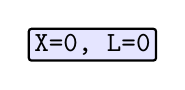
\begin{tikzpicture}[baseline=(b.base)]
				\node[draw=black,line width=0.8pt,fill=blue!10,rectangle,rounded corners=1pt,inner sep=2pt] (b) {\texttt{X=0, L=0}};
			\end{tikzpicture}
		} (state4.west);
		
		% To responses
		\draw[->] (state3) -- (resp0);
		\draw[->] (state4) -- (resp1);
		
	\end{tikzpicture}
	
	\caption{Network System for interleaving executions of the program in Listing~\ref{lst:MotivatingExample3Ser}.}
\label{fig:code3ExampleNS}
\end{figure}



%\begin{figure}[!htbp]
%	\centering
%	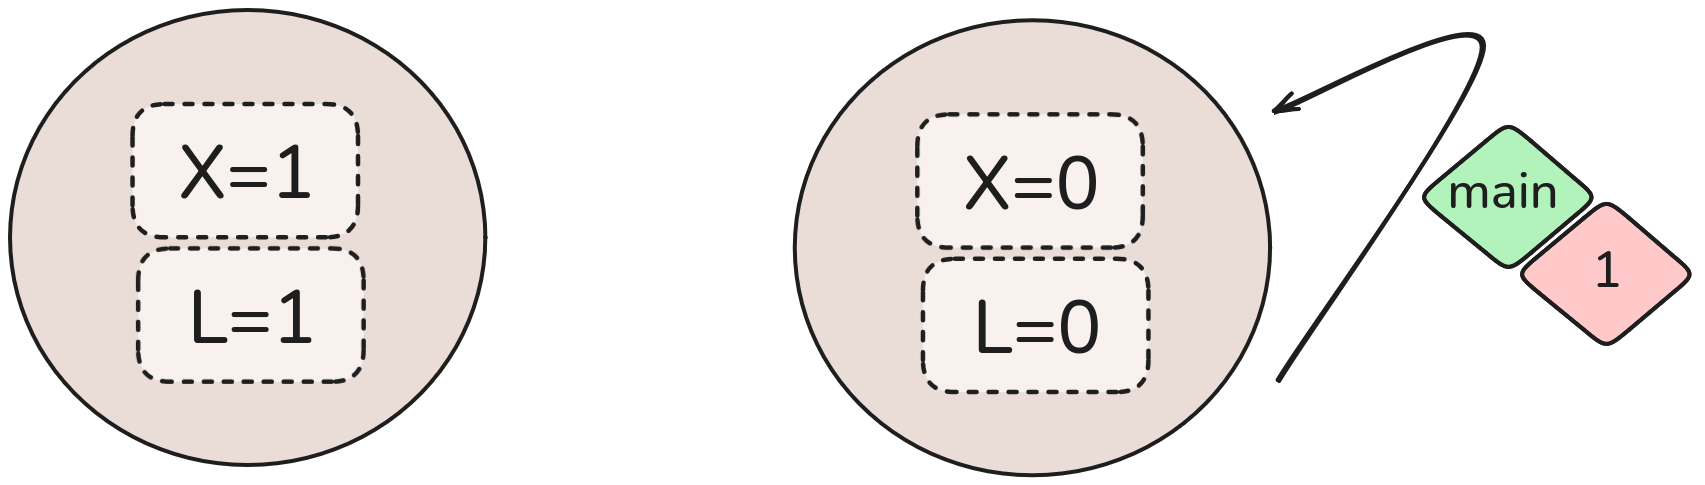
\includegraphics[width=0.4\textwidth]{plots/code_3_NFA.png}
%	\caption{NFA for serial executions of the program in Listing~\ref{lst:MotivatingExample3Ser}.}
%	\label{fig:code3ExampleNFA}
%\end{figure}


\begin{figure}  [!htbp]
	\centering
	% \includegraphics[width=0.48\textwidth,trim=0 0 0 0,clip]{plots/code_two_states_XL_NFA.pdf}
	
	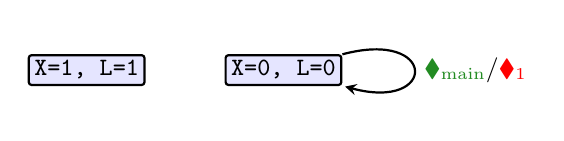
\begin{tikzpicture}[
		->,>=stealth,
		thick,
		node distance=2.5cm,
		state/.style={
			draw=black,
			line width=0.8pt,
			fill=blue!10,
			rectangle,
			rounded corners=1pt,
			inner sep=2pt,
			font=\small
		},
		every node/.style={font=\small}
		]
		% States
		\node[state] (X1L1) {\texttt{X=1, L=1}};
		\node[state, right of=X1L1] (X0L0) {\texttt{X=0, L=0}};
		
		% No edges to or from X=1, L=1 (isolated)
		
		% Self-loop on X=0, L=0 with main/1 (colored lozenge notation)
		\draw[->] (X0L0) edge[loop right]
		node[right] {${\color{ForestGreen}\blacklozenge_{\mathrm{main}}}/{\color{red}\blacklozenge_1}$} (X0L0);
	\end{tikzpicture}
	
	\caption{NFA for serial executions of the program in Listing~\ref{lst:MotivatingExample3Ser}.}
\label{fig:code3ExampleNFA}
\end{figure}




\begin{figure}[!htbp]
	\centering
	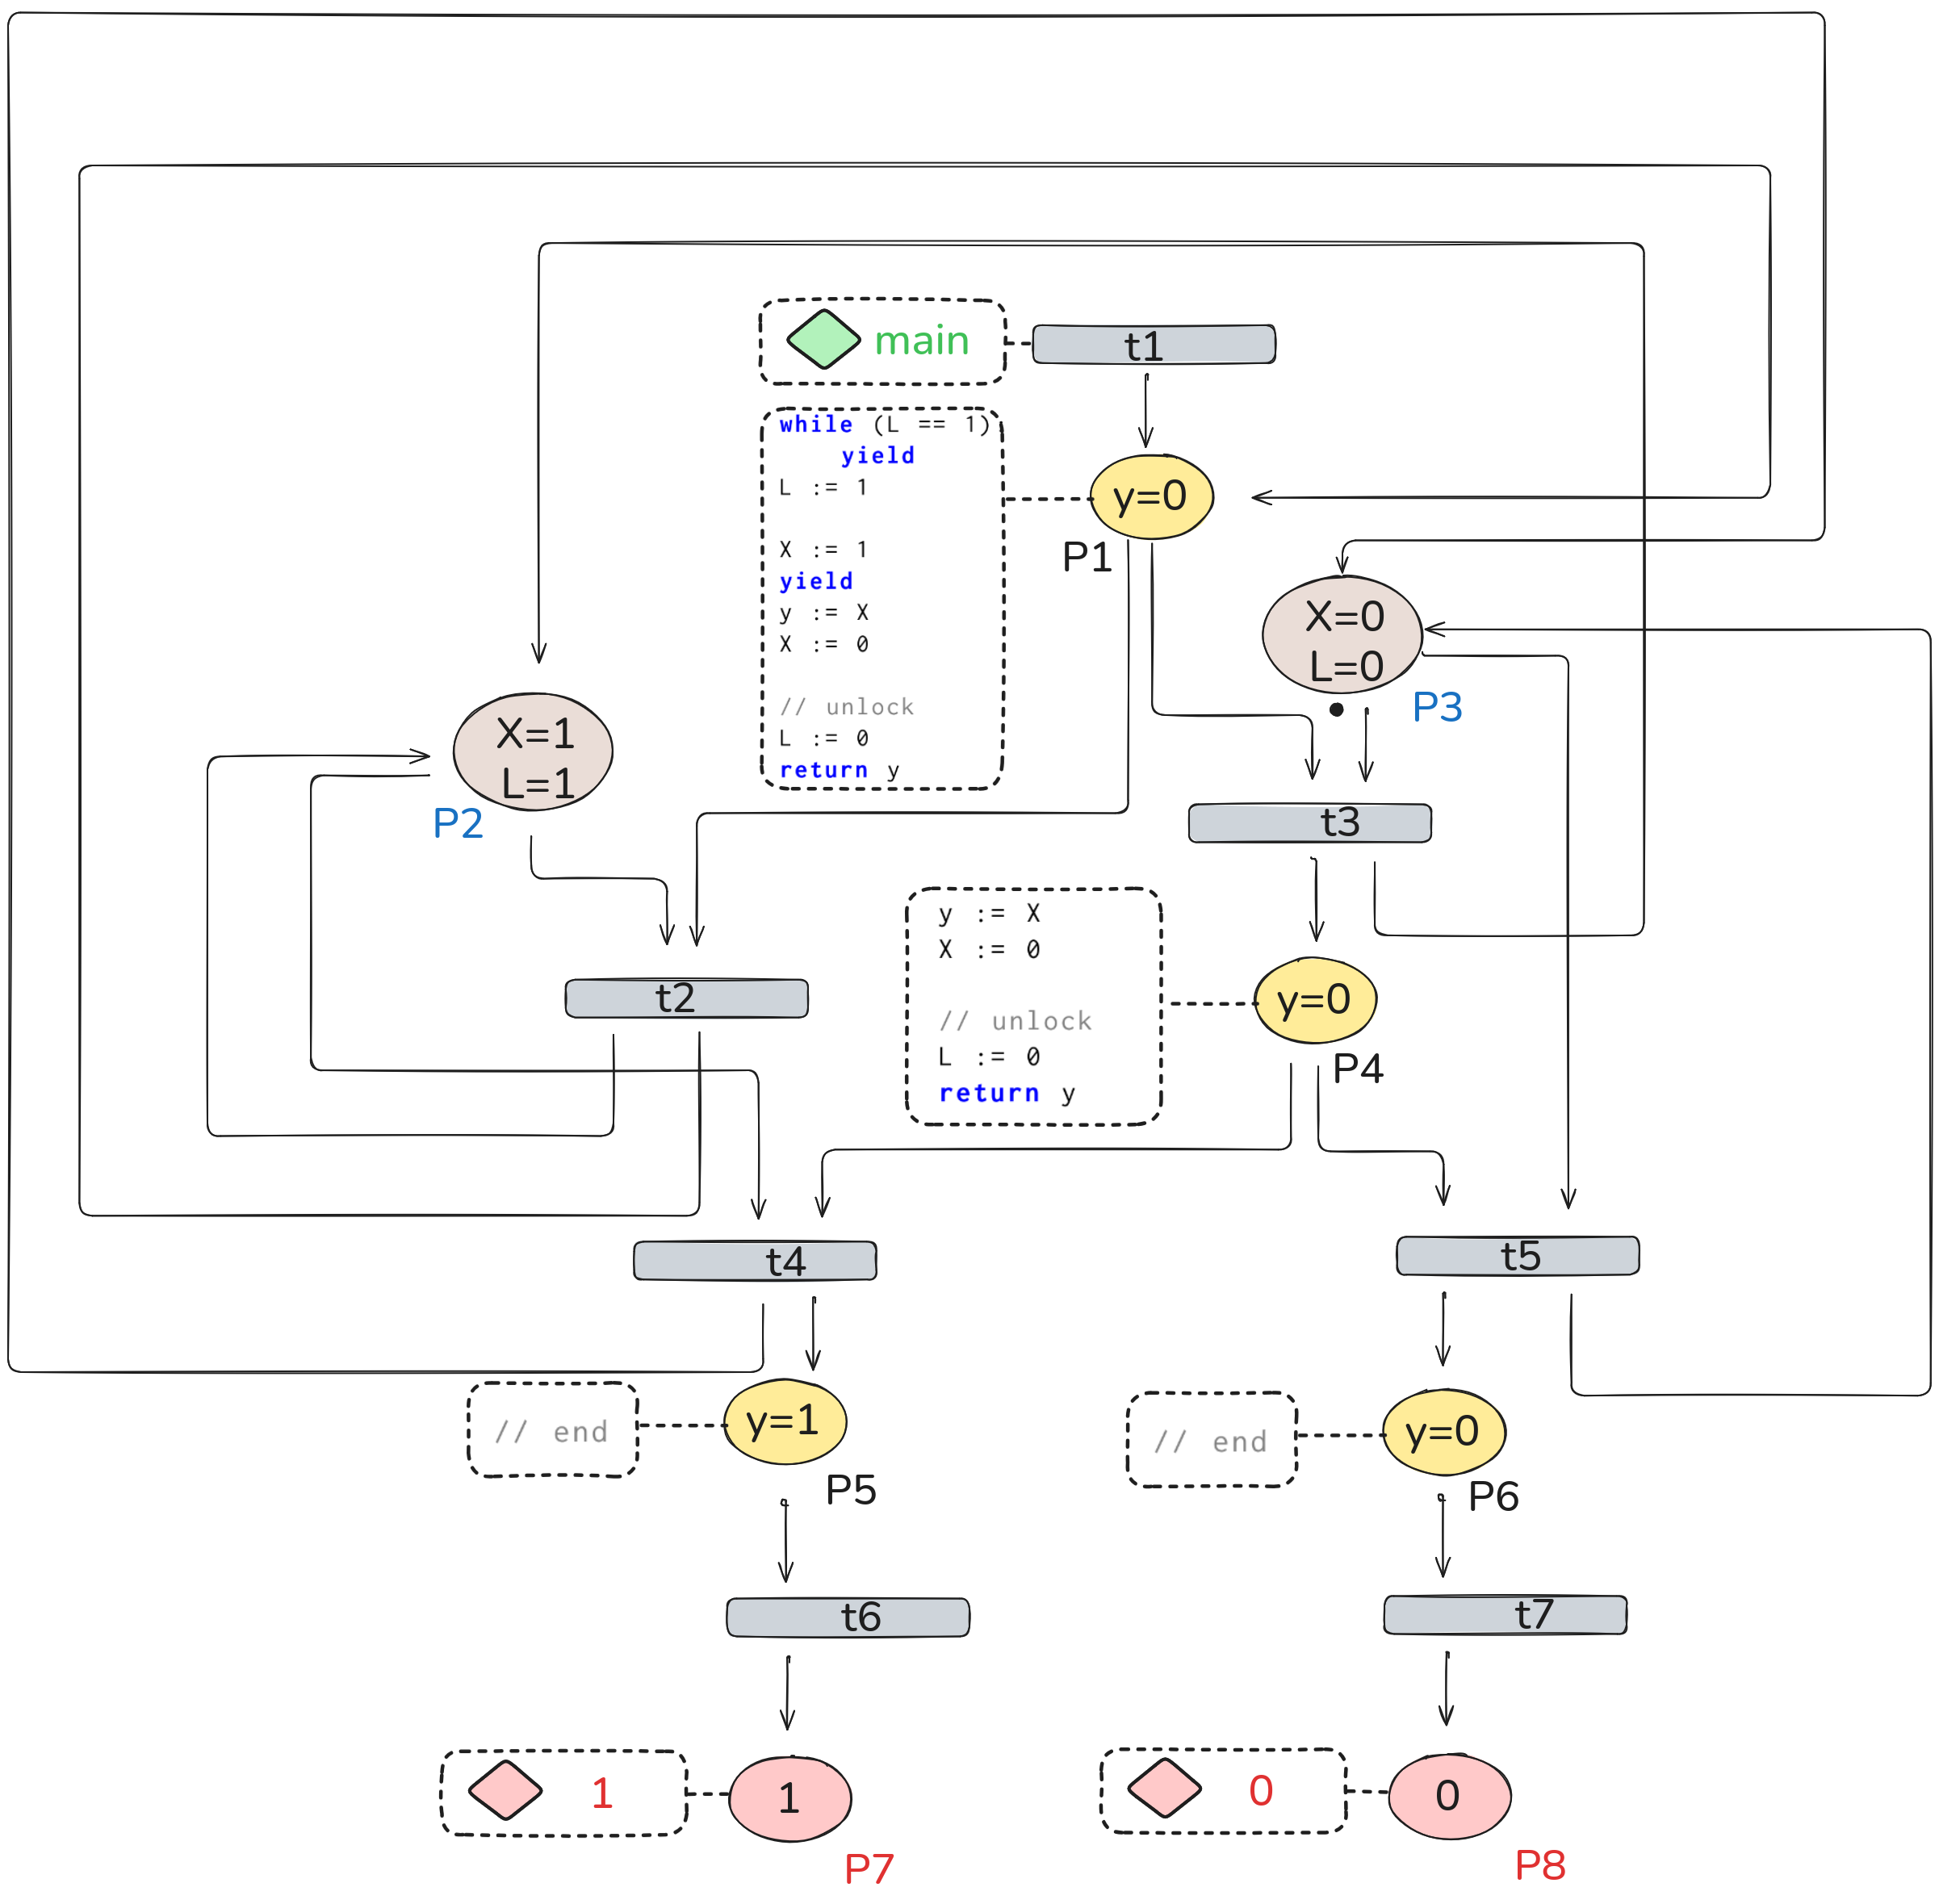
\includegraphics[width=0.8\textwidth]{plots/code_3_PN_with_annotation.png}
	\caption{Petri Net for interleaving executions of the program in Listing~\ref{lst:MotivatingExample3Ser}.}
	\label{fig:code3ExamplePN}
\end{figure}

%\newpage
\section{Ser to NS}
\label{appendix:delta-req-resp-examples}

\begin{figure}[!htbp]
	\centering
	%–––– Network system diagram ––––
	% 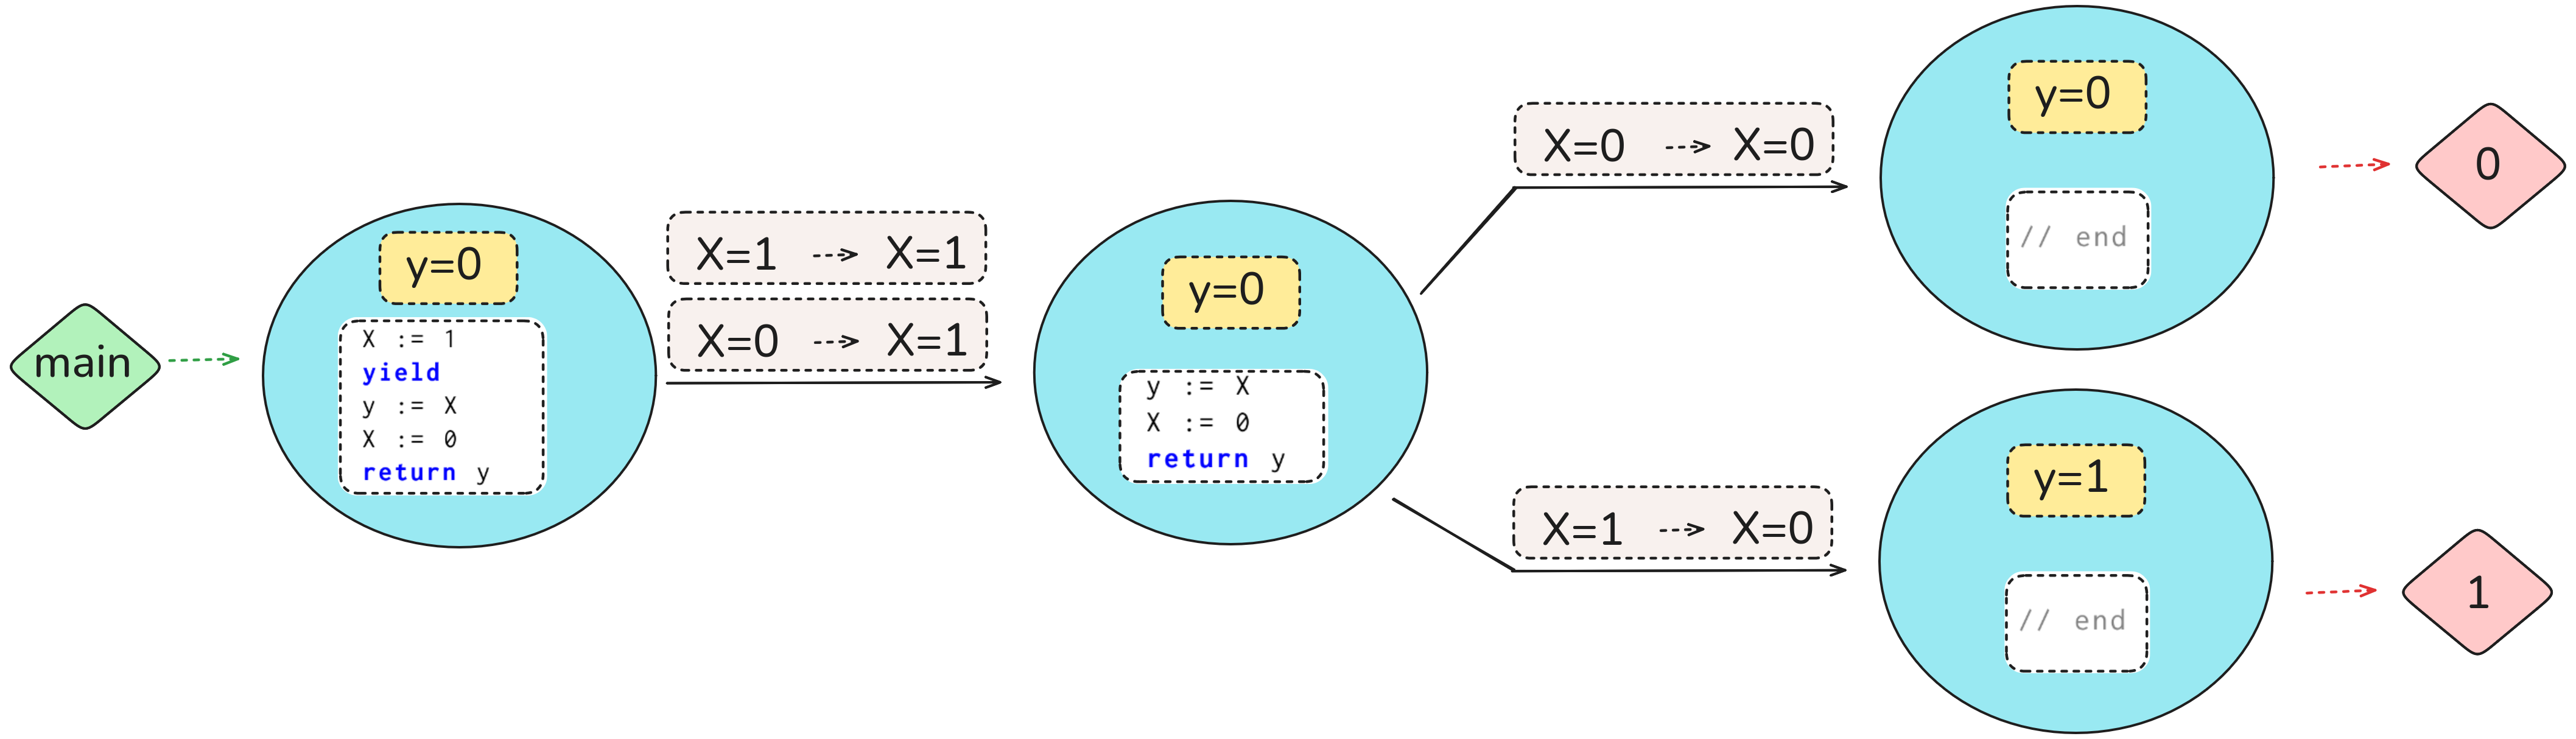
\includegraphics[width=\textwidth]{plots/code_2_NS.png}\\[1ex]
	
	%–––– req, resp, and δ definitions ––––
	\[
	\begin{array}{@{}r@{\;}l}
		req \coloneq & 
		\big\{
		\big[
		\begin{array}{c c c}
			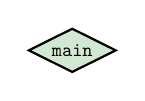
\begin{tikzpicture}[baseline=(textnode.base)]
				\node[
				draw=black,
				line width=0.8pt,
				fill=ForestGreen!20,
				text=black,
				diamond,
				aspect=2,
				inner sep=2pt,
				scale=0.7
				] (textnode) {\texttt{main}};
			\end{tikzpicture}
			&\!\!\rightarrow\!\!&
			\begin{array}{c}
				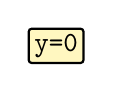
\begin{tikzpicture}[baseline=(ybox.base)]
					\node[
					draw=black,
					line width=0.8pt,
					fill=brightyellow,
					text=black,
					rectangle,
					rounded corners=1pt,
					inner sep=2pt
					] (ybox) {\texttt{y=0}};
				\end{tikzpicture}\vspace{-2pt}
				\\
				\begin{minipage}{0.20\linewidth}
					\begin{lstlisting}[language=CustomPseudoCode,numbers=none,basicstyle=\tiny\ttfamily]
						X := 1 
						yield 
						y := X
						X := 0
						return y
					\end{lstlisting}
				\end{minipage}
			\end{array}
		\end{array}
		\big]
		\big\}
		\\[2em]
		resp \coloneq &
		\big\{
		\big[
		\begin{array}{c c c}
			\begin{array}{c}
				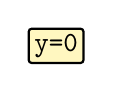
\begin{tikzpicture}[baseline=(ybox.base)]
					\node[
					draw=black,
					line width=0.8pt,
					fill=brightyellow,
					text=black,
					rectangle,
					rounded corners=1pt,
					inner sep=2pt
					] (ybox) {\texttt{y=0}};
				\end{tikzpicture}\vspace{-2pt}
				\\
				\begin{minipage}{0.11\linewidth}
					\begin{lstlisting}[language=CustomPseudoCode,numbers=none,basicstyle=\tiny\ttfamily]
						// end
					\end{lstlisting}
				\end{minipage}
			\end{array}
			&\!\!\rightarrow\!\!&
			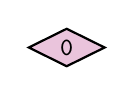
\begin{tikzpicture}[baseline=(textnode.base),scale=0.7]
				\node[
				draw=black,
				line width=0.8pt,
				fill=RedViolet!20,
				text=black,
				diamond,
				aspect=2,
				inner sep=2pt,
				font=\small
				] (textnode) {\texttt{0}};
			\end{tikzpicture}
		\end{array}
		\big]\,{},
		\big[
		\begin{array}{c c c}
			\begin{array}{c}
				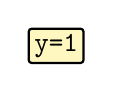
\begin{tikzpicture}[baseline=(ybox.base)]
					\node[
					draw=black,
					line width=0.8pt,
					fill=brightyellow,
					text=black,
					rectangle,
					rounded corners=1pt,
					inner sep=2pt
					] (ybox) {\texttt{y=1}};
				\end{tikzpicture}\vspace{-2pt}
				\\
				\begin{minipage}{0.11\linewidth}
					\begin{lstlisting}[language=CustomPseudoCode,numbers=none,basicstyle=\tiny\ttfamily]
						// end
					\end{lstlisting}
				\end{minipage}
			\end{array}
			&\!\!\rightarrow\!\!&
			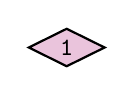
\begin{tikzpicture}[baseline=(textnode.base),scale=0.7]
				\node[
				draw=black,
				line width=0.8pt,
				fill=RedViolet!20,
				text=black,
				diamond,
				aspect=2,
				inner sep=2pt,
				font=\small
				] (textnode) {\texttt{1}};
			\end{tikzpicture}
		\end{array}
		\big]
		\big\}
		\\[2em]
		\delta \coloneq & 
		\big\{\big[(
		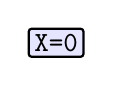
\begin{tikzpicture}[baseline=(ybox.base)]
			\node[
			draw=black,
			line width=0.8pt,
			fill=blue!10,
			text=black,
			rectangle,
			rounded corners=1pt,
			inner sep=2pt
			] (ybox) {\texttt{X=0}};
		\end{tikzpicture}\,{},
		\begin{array}{c}
			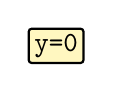
\begin{tikzpicture}[baseline=(ybox.base)]
				\node[
				draw=black,
				line width=0.8pt,
				fill=brightyellow,
				text=black,
				rectangle,
				rounded corners=1pt,
				inner sep=2pt
				] (ybox) {\texttt{y=0}};
			\end{tikzpicture}\vspace{-2pt}
			\\
			\begin{minipage}{0.14\linewidth}
				\begin{lstlisting}[language=CustomPseudoCode,numbers=none,basicstyle=\tiny\ttfamily]
					X := 1
					yield
					y := X
					X := 0
					return y
				\end{lstlisting}
			\end{minipage}
		\end{array}
		)
		\;\rightarrow\;
		(
		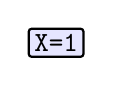
\begin{tikzpicture}[baseline=(ybox.base)]
			\node[
			draw=black,
			line width=0.8pt,
			fill=blue!10,
			text=black,
			rectangle,
			rounded corners=1pt,
			inner sep=2pt
			] (ybox) {\texttt{X=1}};
		\end{tikzpicture}\,{},
		\begin{array}{c}
			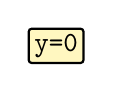
\begin{tikzpicture}[baseline=(ybox.base)]
				\node[
				draw=black,
				line width=0.8pt,
				fill=brightyellow,
				text=black,
				rectangle,
				rounded corners=1pt,
				inner sep=2pt
				] (ybox) {\texttt{y=0}};
			\end{tikzpicture}\vspace{-2pt}
			\\
			\begin{minipage}{0.14\linewidth}
				\begin{lstlisting}[language=CustomPseudoCode,numbers=none,basicstyle=\tiny\ttfamily]
					y := X
					X := 0
					return y
				\end{lstlisting}
			\end{minipage}
		\end{array}
		)
		\big],
		\\[0.5em]
		& \phantom{\big\{}
		\big[(
		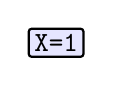
\begin{tikzpicture}[baseline=(ybox.base)]
			\node[
			draw=black,
			line width=0.8pt,
			fill=blue!10,
			text=black,
			rectangle,
			rounded corners=1pt,
			inner sep=2pt
			] (ybox) {\texttt{X=1}};
		\end{tikzpicture}\,{},
		\begin{array}{c}
			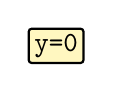
\begin{tikzpicture}[baseline=(ybox.base)]
				\node[
				draw=black,
				line width=0.8pt,
				fill=brightyellow,
				text=black,
				rectangle,
				rounded corners=1pt,
				inner sep=2pt
				] (ybox) {\texttt{y=0}};
			\end{tikzpicture}\vspace{-2pt}
			\\
			\begin{minipage}{0.14\linewidth}
				\begin{lstlisting}[language=CustomPseudoCode,numbers=none,basicstyle=\tiny\ttfamily]
					y := X
					X := 0
					return y
				\end{lstlisting}
			\end{minipage}
		\end{array}
		)
		\;\rightarrow\;
		(
		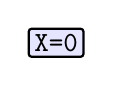
\begin{tikzpicture}[baseline=(ybox.base)]
			\node[
			draw=black,
			line width=0.8pt,
			fill=blue!10,
			text=black,
			rectangle,
			rounded corners=1pt,
			inner sep=2pt
			] (ybox) {\texttt{X=0}};
		\end{tikzpicture}\,{},
		\begin{array}{c}
			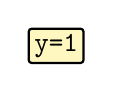
\begin{tikzpicture}[baseline=(ybox.base)]
				\node[
				draw=black,
				line width=0.8pt,
				fill=brightyellow,
				text=black,
				rectangle,
				rounded corners=1pt,
				inner sep=2pt
				] (ybox) {\texttt{y=1}};
			\end{tikzpicture}
			\vspace{-2pt}
			\\
			\begin{minipage}{0.11\linewidth}
				\begin{lstlisting}[language=CustomPseudoCode,numbers=none,basicstyle=\tiny\ttfamily]
					// end
				\end{lstlisting}
			\end{minipage}
		\end{array}
		)
		\big],
		\ldots
		\big\}
	\end{array}
	\]
	\caption{The \(\delta\) transition function, and the \(req\) and \(res\) mappings for the program in Listing~\ref{lst:MotivatingExample2NonSer}.}
	\label{fig:code2ExampleNSSecondPart}
\end{figure}

\clearpage
\section{Translating Network Systems to Petri Nets}
\label{appendix:NS-to-PN-formulation}


We denote with \(\mathbf0\) a zero vector of dimension \(|P|\), and with \(\mathbf1_{p}\) a \(|P|\)-sized indicator vector that has 0 in every coordinate except the one corresponding to place \(p \in P\), which has 1. 
% 
Pre/post maps $\mathsf{pre},\mathsf{post}:T\to\{0,1\}^{|P|}$ assign to each transition $t$ a binary vector over $P$ whose $1$-entries mark the places from which tokens are consumed (for $\mathsf{pre}(t)$) and to which tokens are produced (for $\mathsf{post}(t)$) when $t$ fires.
A transition $t$ is enabled at $M$ iff $\mathsf{pre}(t)\le M$ (component-wise); firing yields
\(
M\xrightarrow{t}M' \quad\text{where}\quad M' = M-\mathsf{pre}(t)+\mathsf{post}(t)
\).	

\medskip
\textit{Construction.}
We generate the Petri net:
\[
N_{\mathrm{int}}(\mathcal S)
= (P,\,T,\,\mathsf{pre},\,\mathsf{post},\,M_0),
\]
where
\[
P
=
P_G \;\cup\; P_{REQ,L} \;\cup\; P_{REQ,RESP}
\]

for 
\[
\begin{aligned}
	P_G
	&= \{\,p_g \mid g\in G\},\quad
	P_{REQ,L}
	= \bigl\{\,p_{({\color{ForestGreen}\blacklozenge_{\mathit{req}}},\ell)}
	\mid {\color{ForestGreen}\blacklozenge_{\mathit{req}}}\in\mathit{REQ},\,\ell\in  L\bigr\},\\[1ex]
	P_{REQ,RESP}
	&= \bigl\{\,p_{({\color{ForestGreen}\blacklozenge_{\mathit{req}}}/{\color{red}\blacklozenge_{\mathit{resp}}})}
	\mid {\color{ForestGreen}\blacklozenge_{\mathit{req}}}\in\mathit{REQ},\,
	{\color{red}\blacklozenge_{\mathit{resp}}}\in\mathit{RESP}\bigr\}.
\end{aligned}
\]


%	\[
%	\begin{aligned}
	%		P_G &= \{\,p_g \mid g\in G\},\;\,
	%		P_{REQ,L} = \{\,p_{{\color{ForestGreen}\blacklozenge_{\mathit{req}}}/\ell}
	%		\mid {\color{ForestGreen}\blacklozenge_{\mathit{req}}}\in\mathit{REQ},\,\ell\in L\},\\
	%		P_{REQ,RESP} &= \{\,p_{{\color{ForestGreen}\blacklozenge_{\mathit{req}}}/{\color{red}\blacklozenge_{\mathit{resp}}}}
	%		\mid {\color{ForestGreen}\blacklozenge_{\mathit{req}}}\in\mathit{REQ},\,
	%		{\color{red}\blacklozenge_{\mathit{resp}}}\in\mathit{RESP}\}.
	%	\end{aligned}
%	\]

%	\[
%	P_G 
%	= \{\,p_g \mid g\in G\}
%	\quad 
%%	P_L 
%%	= \{\,p_\ell \mid \ell\in L\}
%%	\quad
%	P_{REQ,L} =
%	\{\,p_{{\color{ForestGreen}\blacklozenge_{\mathit{req}}}/\ell} \mid
%	{\color{ForestGreen}\blacklozenge_{\mathit{req}}}\in \mathit{REQ}, \ell\in L\},%\\
%	\quad
%	P_{REQ,RESP}=
%	\{\,p_{{\color{ForestGreen}\blacklozenge_{\mathit{req}}}/{\color{red}\blacklozenge_{\mathit{resp}}}} \mid
%	{\color{ForestGreen}\blacklozenge_{\mathit{req}}}\in \mathit{REQ}, {\color{red}\blacklozenge_{\mathit{resp}}}\in \mathit{RESP}\},
%	\]
%	\{\,p_{{\color{ForestGreen}\blacklozenge_{\mathit{req}}}/{\color{red}\blacklozenge_{\mathit{resp}}}} \mid
%	{\color{ForestGreen}\blacklozenge_{\mathit{req}}}\in \mathit{REQ}, {\color{red}\blacklozenge_{\mathit{resp}}}\in \mathit{RESP}\},
%	\]

%	\[
%	P_{REQ,RESP}=
%	\{\,p_{{\color{ForestGreen}\blacklozenge_{\mathit{req}}}/{\color{red}\blacklozenge_{\mathit{resp}}}} \mid
%	{\color{ForestGreen}\blacklozenge_{\mathit{req}}}\in \mathit{REQ}, {\color{red}\blacklozenge_{\mathit{resp}}}\in \mathit{RESP}\},
%	\]

with \(G\) being the set of global states, \(L\) being the set of local states (in the case of a \toolname-derived NS, this is the coupling of the local variable assignments of an in-flight request and its remaining \toolname{} program to execute), \(\mathit{REQ}\) denotes the request labels; and \(\mathit{RESP}\) denotes the response labels.

\medskip
Transitions are partitioned as:
\[
T = T_{\mathit{req}} \;\cup\; T_{\delta}\;\cup\;T_{\mathit{resp}}
\]
where

%	\[
%	T_{\mathit{req}} = \{\,t_{({\color{ForestGreen}\blacklozenge_{\mathit{req}}},\ell)} \mid {(\color{ForestGreen}\blacklozenge_{\mathit{req}}},\ell)\in\mathit{req}\},\quad
%	T_{\delta} = \{\,t_{(\ell,g)\to(\ell',g')} \mid (\ell,g)\xrightarrow{}(\ell',g')\in\delta\},\quad
%	T_{\mathit{resp}} = \{\,t_{(\ell,{\color{red}\blacklozenge_{\mathit{resp}}})} \mid (\ell,{\color{red}\blacklozenge_{\mathit{resp}}})\in\mathit{resp}\}.
%	\]

\begin{align*}
	T_{\mathit{req}}
	&= \{\,t_{({\color{ForestGreen}\blacklozenge_{\mathit{req}}},\ell)} \mid {(\color{ForestGreen}\blacklozenge_{\mathit{req}}},\ell)\in\mathit{req}\},\\[1ex]
	T_{\delta}
	&= \bigl\{\,t_{((\ell,g),(\ell',g'))} 
	\mid ((\ell,g),(\ell',g'))\in\delta\bigr\},\quad
	T_{\mathit{resp}}
	= \{\,t_{(\ell,{\color{red}\blacklozenge_{\mathit{resp}}})} \mid (\ell,{\color{red}\blacklozenge_{\mathit{resp}}})\in\mathit{resp}\}.
\end{align*}



%\smallskip
%Given a local state \(\ell\) which resulted from a request \({\color{ForestGreen}\blacklozenge_{\mathit{req}}}\) (either directly or downstream due to program execution) --- the transitions are:
Their \(\mathsf{pre}\) and \(\mathsf{post}\) mappings are:
\[
\begin{alignedat}{3}
	\mathsf{pre}\bigl(t_{({\color{ForestGreen}\blacklozenge_{\mathit{req}}},\ell)}\bigr)
	&= \mathbf0, &
	\mathsf{post}\bigl(t_{({\color{ForestGreen}\blacklozenge_{\mathit{req}}},\ell)}\bigr)
	&= \mathbf1_{p_{({\color{ForestGreen}\blacklozenge_{\mathit{req}}},\ell)}}, 
	&&\text{for }({\color{ForestGreen}\blacklozenge_{\mathit{req}}},\ell)\in\mathit{req},\\
	\mathsf{pre}\bigl(t_{((\ell,g),(\ell',g'))}\bigr)
	&= \mathbf1_{p_{({\color{ForestGreen}\blacklozenge_{\mathit{req}}},\ell)}} + \mathbf1_{p_g}, &
	\mathsf{post}\bigl(t_{((\ell,g),(\ell',g'))}\bigr)
	&= \mathbf1_{p_{({\color{ForestGreen}\blacklozenge_{\mathit{req}}},\ell')}} + \mathbf1_{p_{g'}}, 
	&&\text{for }{{\color{ForestGreen}\blacklozenge_{\mathit{req}}}\in\mathit{REQ}}, ((\ell,g),(\ell',g'))\in\delta,\\
	\mathsf{pre}\bigl(t_{(\ell,{\color{red}\blacklozenge_{\mathit{resp}}})}\bigr)
	&= \mathbf1_{p_{({\color{ForestGreen}\blacklozenge_{\mathit{req}}},\ell)}}, &
	\mathsf{post}\bigl(t_{(\ell,{\color{red}\blacklozenge_{\mathit{resp}}})}\bigr)
	&= \mathbf1_{p_{({\color{ForestGreen}\blacklozenge_{\mathit{req}}}/{\color{red}\blacklozenge_{\mathit{resp}}})}}, 
	&&\text{for }{{\color{ForestGreen}\blacklozenge_{\mathit{req}}}\in\mathit{REQ},(\ell,\color{red}\blacklozenge_{\mathit{resp}}})\in\mathit{resp}
	%\ %(\ell\text{ the matching local state).
		%		}
\end{alignedat}
\]

Where for the last two cases, \({\color{ForestGreen}\blacklozenge_{\mathit{req}}}\) concerns requests that eventually give rise to a local state \(\ell \in L\) that originated downstream (during execution).

\medskip
The initial marking is a single token on the place representing the initial global state $g_0$ of the NS:
\[
M_0(p_{g_0}) = 1,
\quad
M_0(p) = 0 \text{ for all }p\neq p_{g_0},
\]
%	where \(g_0\) is the initial global state of the network system \(\mathcal S\).  



Define the projection \(\pi\) to solely include the markings of places representing completed request/response pairs.
% (with the exception of a single token on a state in \(P_G\)).
%\[
%\pi \;:\;\mathbb N^P \;\longrightarrow\;\mathbb N^{P_R}
%\quad\bigl(\pi(M)\bigr)(p_{({{\color{ForestGreen}\blacklozenge_{\mathit{req}}}/{\color{red}\blacklozenge_{\mathit{resp}}}})})\;=\;M(p_{({{\color{ForestGreen}\blacklozenge_{\mathit{req}}}/{\color{red}\blacklozenge_{\mathit{resp}}}})})\text{ for }p_{({{\color{ForestGreen}\blacklozenge_{\mathit{req}}}/{\color{red}\blacklozenge_{\mathit{resp}}}})}\in P_{REQ,RESP}.
%\]
Then, the multiset of all  (${{\color{ForestGreen}\blacklozenge_{\mathit{req}}}/{\color{red}\blacklozenge_{\mathit{resp}}}}$) pairs of the NS, obtained by \textit{any} interleaving, is:
\[
\mathsf{Int}(\mathcal S)
\;=\;
\bigl\{\;\pi(M)\;\bigm|\;M_0 \xrightarrow{}^{*} M\text{ in }N_{\mathrm{int}}(\mathcal S)\bigr\}.
\]

\section{Example: Serializable Program}
\label{appendix:ns-serializable}


Now, we observe again the adjusted program with a spin-lock (as previously described in Listing~\ref{lst:MotivatingExample3Ser}), of which we depicted figures of the corresponding Network System (Fig.~\ref{fig:code3ExampleNS}), the Serializability NFA (Fig.~\ref{fig:code3ExampleNFA}), and the Interleaving Petri net (Fig.~\ref{fig:code3ExamplePN}) in Appendix~\ref{appendix:MoreNsExamples}.
%
In this case, serializability corresponds to the Petri net being unable to reach a marking satisfying the same semilinear formula \(\mathcal {F}\) as in the non-serializable case described in the main text (subsec.~\ref{subsec:SerToNsTranslation}):

\[
\mathcal {F}:
\quad
P_1 = 0 \wedge 
\textcolor{blue}{P_2} \ge 0 \wedge \textcolor{blue}{P_3} \ge 0  \wedge P_4 = 0
\wedge P_5 = 0 \wedge P_6 = 0 \wedge \textcolor{red}{P_7} \ge 0 \wedge \textcolor{red}{P_8} \ge 1.
\]

% (note however, that this is not always the case). 
%(but this time each place $P_i$ corresponds to the new PN). 
%following formula:
%
%\[
%\textcolor{blue}
%P_1 = 0 \wedge 
%{P_2} \ge 0 \wedge \textcolor{blue}{P_3} \ge 0  \wedge P_4 = 0
%\wedge P_5 = 0 \wedge P_6 = 0 \wedge \textcolor{red}{P_7} = 0 \wedge \textcolor{red}{P_8} \ge 1.
%\]


In addition, although the target set is the same as in the previous example, the Petri net places $(P_1,\ldots,P_8)$ encode different states that correspond to the updated network system. For instance, now each place in the PN that encodes a global state accounts for two global variables, \texttt{X} and \texttt{L}, and the initial global state corresponds to the place encoding the initial assignment \textcolor{blue}{[X=0, L=0]}, etc.
%
Furthermore, unlike the case in Listing~\ref{lst:MotivatingExample2NonSer} (covered in subsec.~\ref{subsec:SerToNsTranslation}), this target set of markings (encoding request/response pairs of non-serial executions) is \textit{unreachable}, as witnessed by the inductive invariant:


\[
\begin{aligned}
	&(P_{1},\textcolor{blue}{P_{2}},\textcolor{blue}{P_{3}},P_{4},P_{5},P_{6},\textcolor{red}{P_{7}},\textcolor{red}{P_{8}})
	\;\mapsto\;\\
	&\quad
	\exists\,e_{0},\dots,e_{5}\ge0.\;
	\Bigl(
	e_{2}-e_{1}+\textcolor{blue}{P_{3}}-1=0\;\land\;
	e_{2}+P_{1}-e_{5}=0\;\land\;
	P_{5}-e_{1}+e_{4}=0\;\land\\
	&\qquad\quad
	-\,e_{4}+\textcolor{red}{P_{7}}=0\;\land\;
	P_{6}+e_{3}-e_{0}=0\;\land\;
	\textcolor{red}{P_{8}}-e_{3}=0\;\land\\
	&\qquad\quad
	-\,e_{2}+e_{1}+e_{0}+P_{4}=0\;\land\;
	-\,e_{2}+e_{1}+\textcolor{blue}{P_{2}}=0
	\Bigr)
	\;\land\;
	\bigl(P_{4}-1\ge0\;\lor\;\textcolor{blue}{P_{3}}-1\ge0\bigr).
\end{aligned}
\]


We then revert and project it on the request/response pairs of the network system.
%
We get the following inductive invariants for each of the two (reachable) global states:

\begin{proof}
	
	\medskip\noindent
	For global state \textcolor{blue}{[L=0,X=0]} the projected invariant is:
	\[
	\bigl(\,\text{\color{ForestGreen}$\blacklozenge_{\text{main}}$}/\text{\color{red}$\blacklozenge_{0}$},\;
	\text{\color{ForestGreen}$\blacklozenge_{\text{main}}$}/\text{\color{red}$\blacklozenge_{1}$}\bigr)
	\;\mapsto\;
	\exists\,e_{0},\dots,e_{5}\ge0.\;
	\begin{aligned}[t]
		& e_{2}-e_{1}=0,\quad
		e_{2}-e_{5}=0,\quad
		-e_{1}+e_{4}=0,\\
		& -e_{4}+\bigl(\text{\color{ForestGreen}$\blacklozenge_{\text{main}}$}/\text{\color{red}$\blacklozenge_{1}$}\bigr)=0,\quad
		-e_{0}+e_{3}=0,\\
		& -e_{3}+\bigl(\text{\color{ForestGreen}$\blacklozenge_{\text{main}}$}/\text{\color{red}$\blacklozenge_{0}$}\bigr)=0,\quad
		-e_{2}+e_{1}+e_{0}=0,\\
		& -e_{2}+e_{1}=0.
	\end{aligned}
	\]
	\noindent From 
	\[e_{1}=e_{2}=e_{4}=e_{5}=(\;
	\text{\color{ForestGreen}$\blacklozenge_{\text{main}}$}/\text{\color{red}$\blacklozenge_{1}$}),\;
	e_{0}=e_{3}=
	(\text{\color{ForestGreen}$\blacklozenge_{\text{main}}$}/\text{\color{red}$\blacklozenge_{0}$})
	\]
	
	it follows that \[-e_{2}+e_{1}+e_{0}=0\;\Longrightarrow\;e_{0}=0,\]
	
	thus: 
	\[
	(	\text{\color{ForestGreen}$\blacklozenge_{\text{main}}$}/\text{\color{red}$\blacklozenge_{0}$})
	=0 \quad \text{and} \quad (	\text{\color{ForestGreen}$\blacklozenge_{\text{main}}$}/\text{\color{red}$\blacklozenge_{1}$})
	=0
	\]
	
	indicating that  (\(\text{\color{ForestGreen}$\blacklozenge_{\text{main}}$}/\text{\color{red}$\blacklozenge_{0}$}\)) cannot be obtained from the global state
	\textcolor{blue}{[L=0,X=0]}.
	
	\medskip\noindent
	In the second case, for the global state \textcolor{blue}{[L=1, X=1]}
	the projected invariant is:
	
	
	\[
	\bigl(\,\text{\color{ForestGreen}$\blacklozenge_{\text{main}}$}/\text{\color{red}$\blacklozenge_{0}$},\;
	\text{\color{ForestGreen}$\blacklozenge_{\text{main}}$}/\text{\color{red}$\blacklozenge_{1}$}\bigr)
	\;\mapsto\;
	\exists\,e_{0},\dots,e_{5}.\;\bot,
	\]
	which is unsatisfiable. Hence, no completed request/response pair, and in particular, no (\(\text{\color{ForestGreen}$\blacklozenge_{\text{main}}$}/\text{\color{red}$\blacklozenge_{0}$}\)) pair can be produced from this state via \textit{any} execution. Intuitively, this aligns with the fact that there cannot be any output generated via an interleaving, given that the spin-lock is acquired (\textcolor{blue}{[L=1]}).
	%	\guy{Mark/Jules is this part correct?}
	
	\medskip
	\noindent\textbf{Conclusion.}
	In every reachable state, no request/response pair of type	($	\text{\color{ForestGreen}$\blacklozenge_{\text{main}}$}/\text{\color{red}$\blacklozenge_{0}$})
	$
	can occur. Consequently, the only possible pairs are of type
	($	\text{\color{ForestGreen}$\blacklozenge_{\text{main}}$}/\text{\color{red}$\blacklozenge_{1}$})
	$,
	all of which lie within the NFA’s language for serial executions (Fig.~\ref{fig:code3ExampleNFA}).
	Hence, the program is serializable. Moreover, as proven in subsection~\ref{appendix:subsec:InductiveInvariantExample},
	these invariants are inductive: they hold in the initial state and are preserved under every transition.
\end{proof}

%	\medskip\noindent
%	\textbf{Conclusion.}
%	In all reachable states
%	it holds that there cannot be any request/response pair of type
%	(	$	\text{\color{ForestGreen}$\blacklozenge_{\text{main}}$}/\text{\color{red}$\blacklozenge_{0}$}
%	$).
%	%
%	Furthermore, this indicates that the only attainable request/response pairs are of the form 	($	\text{\color{ForestGreen}$\blacklozenge_{\text{main}}$}/\text{\color{red}$\blacklozenge_{1}$})
%	$, which are included in the language of of NFA for serial executions. Thus, this program is serializable.
%	%
%	We further show (in Appendix~\ref{appendix:InductiveInvariantExample}) that these invariants are \textit{inductive}: they encompass the system’s initial state and, once satisfied, remain true for all subsequent executions.




%\newpage


%\subsection{Time/Space Complexity}
%
%\guy{Should we add something about time/space complexity?}

%\newpage

\subsection{Proof of Inductive Invariant}
\label{appendix:subsec:InductiveInvariantExample}


\begin{proof}
	
	Define the predicate
	\[
	\begin{aligned}
		I(P_{1},\dots,\textcolor{red}{P_{8}})
		:={}&
		(P_{1},\textcolor{blue}{P_{2}},\textcolor{blue}{P_{3}},P_{4},P_{5},P_{6},\textcolor{red}{P_{7}},\textcolor{red}{P_{8}})
		\;\mapsto\;\\
		&\quad
		\exists\,e_{0},\dots,e_{5}\ge0.\;
		\Bigl(
		e_{2}-e_{1}+\textcolor{blue}{P_{3}}-1=0\;\land\;
		e_{2}+P_{1}-e_{5}=0\;\land\;
		P_{5}-e_{1}+e_{4}=0\;\land\\
		&\qquad\quad
		-\,e_{4}+\textcolor{red}{P_{7}}=0\;\land\;
		P_{6}+e_{3}-e_{0}=0\;\land\;
		\textcolor{red}{P_{8}}-e_{3}=0\;\land\\
		&\qquad\quad
		-\,e_{2}+e_{1}+e_{0}+P_{4}=0\;\land\;
		-\,e_{2}+e_{1}+\textcolor{blue}{P_{2}}=0
		\Bigr)
		\;\land\;
		\bigl(P_{4}-1\ge0\;\lor\;\textcolor{blue}{P_{3}}-1\ge0\bigr).
	\end{aligned}
	\]
	
	
	\medskip\noindent
	\textbf{(1) Initialization.}
	The initial marking has $\textcolor{blue}{P_{3}}=1$ and $P_{1}=\textcolor{blue}{P_{2}}=P_{4}=P_{5}=P_{6}=\textcolor{red}{P_{7}}=\textcolor{red}{P_{8}}=0$.
	Choose $e_{0}=\cdots=e_{5}=0$.  Then
	\[
	e_{i}\ge0,\quad
	e_{2}-e_{1}+\textcolor{blue}{P_{3}}-1=0-0+1-1=0,\;\dots,\;-e_{2}+e_{1}+P_{2}=0,
	\]
	and 
	\[
	P_{4}-1\ge0\;\lor\;\textcolor{blue}{P_{3}}-1\ge0
	\;=\;-1\ge0\;\lor\;0\ge0
	\;=\;\texttt{FALSE}\;\lor\;\texttt{TRUE}
	\;=\;\texttt{TRUE}.
	\]
	Thus $I$ holds initially.
	
	\medskip\noindent
	\textbf{(2) Consecution.}
	One checks for each transition $t_{k}$ of the Petri net that
	\[
	I(M)\;\Longrightarrow\;I\bigl(t_{k}(M)\bigr).
	\]
	In each case, the same $(e_{0},\dots,e_{5})$ can be adjusted (per the \texttt{SMT} certificate) to show that the eight equalities and the disjunction remain valid. See our accompanying artifact~\cite{ArtifactRepository} for generating a full proof in the standard \texttt{SMT-LIB} format~\cite{BaStTi10}.
	
	\medskip\noindent
	\textbf{(3) Refutation of the property.}
	Suppose by contradiction that there exists a marking $P$ for which both $I(P)$ and $\mathcal {F}(P)$ hold:
	\[
	\mathcal {F}(P):\quad
	P_{1}=0,\;
	\textcolor{blue}{P_{2}}\ge0,\;
	\textcolor{blue}{P_{3}}\ge0,\;
	P_{4}=0,\;
	P_{5}=0,\;
	P_{6}=0,\;
	\textcolor{red}{P_{7}}\ge0,\;
	\textcolor{red}{P_{8}}\ge1.
	\] 
	
	\noindent
	From
	\[
	e_{2}-e_{1}+\textcolor{blue}{P_{3}}-1=0
	\quad\text{and}\quad
	-e_{2}+e_{1}+\textcolor{blue}{P_{2}}=0
	\]
	we get
	\[
	\textcolor{blue}{P_{2}}=1-\textcolor{blue}{P_{3}}.
	\]
	From
	\[
	\textcolor{red}{P_{8}}-e_{3}=0
	\quad\text{and}\quad
	P_{6}+e_{3}-e_{0}=0
	\]
	and from the assumption that $P_6=0$, we get
	\[
	e_{0}=e_{3}=\textcolor{red}{P_{8}}.
	\]
	
	
	\noindent
	Similarly, the invariant equalities 
	$(-\,e_{2}+e_{1}+e_{0}+P_{4}=0)$ and $(	-\,e_{2}+e_{1}+\textcolor{blue}{P_{2}}=0)$
	induce
	\[
	\textcolor{blue}{P_{2}}=P_{4}+e_{0}=P_{4}+\textcolor{red}{P_{8}},
	\]
	thus, and as we also assume that $P_4=0$, then:
	\[
	\textcolor{red}{P_{8}}=\textcolor{blue}{P_2}-P4=(1-\textcolor{blue}{P_{3}})-P_{4}=1-\textcolor{blue}{P_{3}}-0=1-\textcolor{blue}{P_{3}}
	\]
	
	
	
	
%	\medskip
	\noindent
	However, $\mathcal {F}(P)$ also induces $\textcolor{blue}{P_{3}}\ge0$ and $\textcolor{red}{P_{8}}\ge1$, and hence $\textcolor{blue}{P_{3}}=0$.  
	Furthermore, as our invariant includes a conjunction with $\bigl(P_{4}-1\ge0\;\lor\;\textcolor{blue}{P_{3}}-1\ge0\bigr)$, then it necessarily holds that \(P_{4}\ge1\). This contradicts \(P_{4}=0\) as required for the semilinear set to be reachable.
	%
	Thus, $I\land\mathcal {F}$ is unsatisfiable, i.e., 
	%\[
	$
	I(P)\;\Longrightarrow\;\neg\mathcal {F}(P)$.
	%\]
	This completes the proof that $I$ is an inductive invariant refuting property $\mathcal {F}$.
\end{proof}


%\newpage

\section{Non-Serializable Execution Counterexample}
\label{appendix:non-serializable-execution-example}
Continuing the running example presented in subsec.~\ref{subsec:SerToNsTranslation}, we present in Table~\ref{tab:PetriNetFiringCounterexample} a firing sequence of the Petri net (Fig.~\ref{fig:code2ExamplePN}) resulting in the marking \(M^*\):

\[
M^* = \{\textcolor{blue}{P_3}(1),\;\textcolor{red}{P_7}(1),\;\textcolor{red}{P_8}(1)\}
\]
%\medskip
%\noindent
%\textbf{Serializable NFA Extraction.}
%%
%
%
%
%\begin{wrapfigure}{r}{0.5\textwidth}  % “r” = right, width = 0.5\textwidth
%	\centering
%	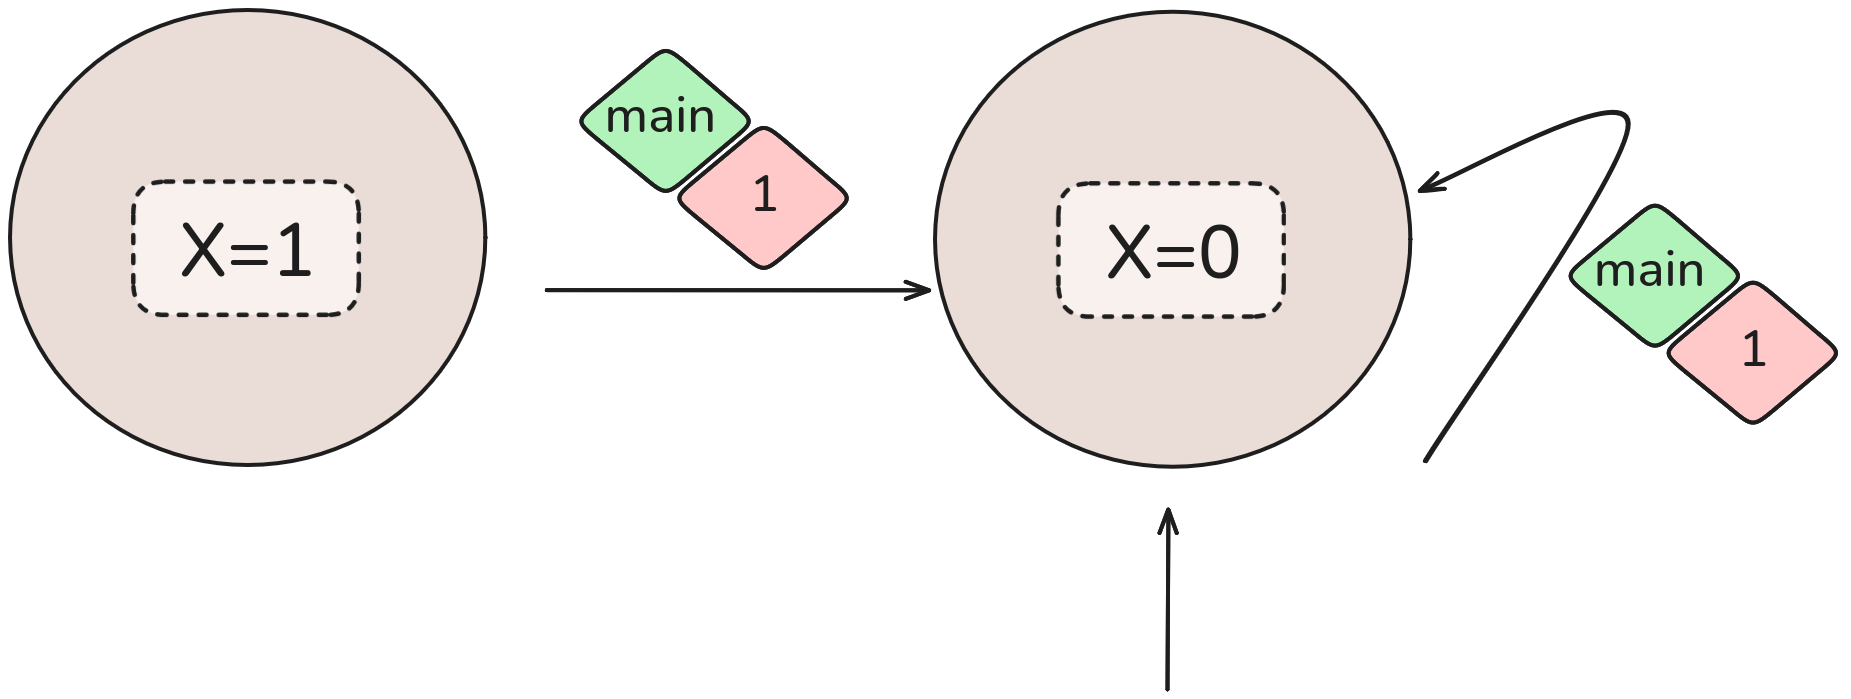
\includegraphics[width=0.48\textwidth,trim=0 0 0 0,clip]{plots/code_2_NFA.png}
%	\caption{NFA for serialized executions of Listing~\ref{lst:MotivatingExample2NonSer}.}
%	\label{fig:code2ExampleNFA}
%\end{wrapfigure}

%\begin{figure}[!htbp]
%	\centering
%	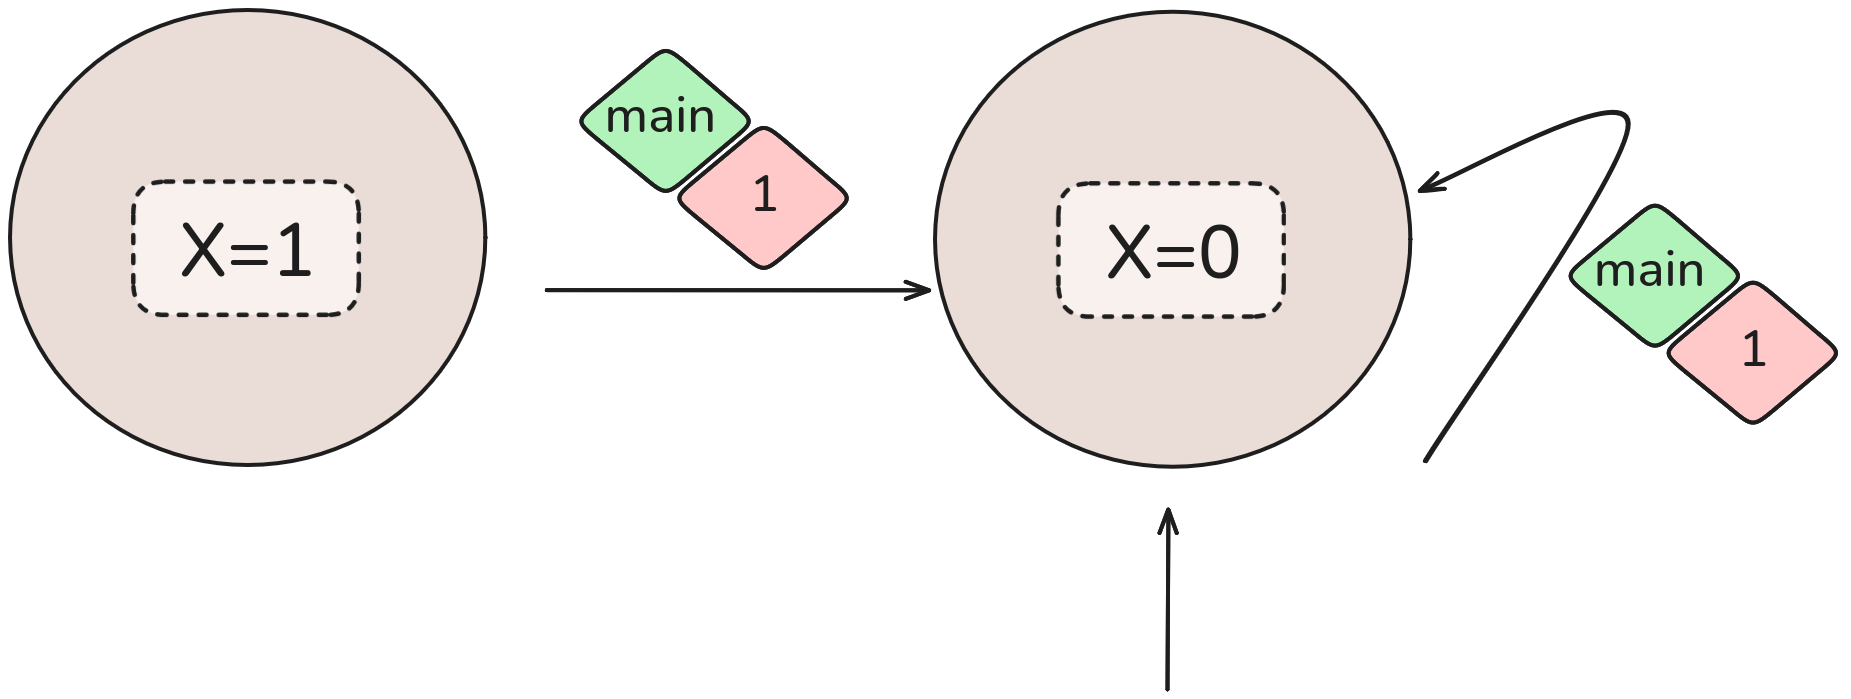
\includegraphics[width=0.5\textwidth,trim=0 0 0 0,clip]{plots/code_2_NFA.png}
%	\caption{NFA for serialized executions of Listing~\ref{lst:MotivatingExample2NonSer}.}
%	\label{fig:code2ExampleNFA}
%\end{figure}
%
%\medskip
%\noindent
%\textbf{Petri Net Extraction.}
%
%
%
%\medskip
%\noindent
%\textbf{Counterexample Extraction.}
%%
%
%%


\begin{table}[H]
	\centering
	\label{tab:reach-seq}
	\resizebox{0.9\textwidth}{!}{
		\begin{tabular}{c l c c c c c c}
			\toprule
			\textbf{Step} 
			& \textbf{Firing} 
			& \multicolumn{3}{c}{\textbf{Marking (after firing)}} 
			& \multicolumn{3}{c}{\textbf{Description (after firing)}} \\
			\cmidrule(lr){3-5} \cmidrule(lr){6-8}
			& 
			& \textbf{Global} 
			& \textbf{Local} 
			& \textbf{Responses} 
			& \textbf{Global state} 
			& \textbf{In-flight requests} 
			& \textbf{Responses} \\
			\midrule
			0 & --                                  
			& {\color{blue}$P_3$(1)}                  
			& --                                    
			& --                                    
			& {\color{blue}[X=0]}                   
			& --                          
			& --                                    \\
			1 & $\textcolor{ForestGreen}{t_1}$ 
			& {\color{blue}$P_3$(1)}                  
			& $P_1$(1)                                
			& --                                    
			& {\color{blue}[X=0]}                   
			& {\color{ForestGreen}$\blacklozenge_\text{main}$} 
			& --                                    \\
			2 & $\textcolor{ForestGreen}{t_1}$ 
			& {\color{blue}$P_3$(1)}                  
			& $P_1$(2)                                
			& --                                    
			& {\color{blue}[X=0]}                   
			& {\color{ForestGreen}$\blacklozenge_\text{main}$}, {\color{ForestGreen}$\blacklozenge_\text{main}$}  
			& --                                    \\
			3 & $t_3$                                  
			& {\color{blue}$P_2$(1)}                  
			& $P_1$(1),$P_4$(1)                          
			& --                                   
			&                                    {\color{blue}[X=1]}    
			&                                    {\color{black}$\blacklozenge_\text{until yield}$}, {\color{ForestGreen}$\blacklozenge_\text{main}$}   
			& --                                    \\
			4 & $t_2$                                  
			& {\color{blue}$P_2$(1)}                  
			& $P_4$(2)                                
			& --                                    
			&                                    {\color{blue}[X=1]}    
			&                                    {\color{black}$\blacklozenge_\text{until yield}$}, {\color{black}$\blacklozenge_\text{until yield}$}   
			& --                                    \\
			5 & $t_4$                                  
			& {\color{blue}$P_3$(1)}                  
			& $P_5$(1),$P_4$(1)                          
			& --                                    
			&                                   {\color{blue}[X=0]}     
			&                                    {\color{black}$\blacklozenge_\text{after yield}$}, {\color{black}$\blacklozenge_\text{until yield}$}   
			& --                                    \\
			6 & $\textcolor{red}{t_6}$                     
			& {\color{blue}$P_3$(1)}                  
			& $P_4$(1)                                
			& {\color{red}$P_7$(1)}                    
			&                                      	{\color{blue}[X=0]}  
			&                                    {\color{black}$\blacklozenge_\text{until yield}$}   
			&                                   {\color{red}$\blacklozenge_1$}     \\
			7 & $t_5$                                  
			& {\color{blue}$P_3$(1)}                  
			& $P_6$(1)                                
			& {\color{red}$P_7$(1)}                    
			&                                   {\color{blue}[X=0]}    
			&                                    {\color{black}$\blacklozenge_\text{after yield}$}      
			&                                   {\color{red}$\blacklozenge_1$}        \\
			8 & $\textcolor{red}{t_7}$                     
			& {\color{blue}$P_3$(1)}                                  
			& --                                    
			& {\color{red}$P_7$(1),\color{red}$P_8$(1)}    
			&                                   {\color{blue}[X=0]}    
			&                                   --    
			&                                   {\color{red}$\blacklozenge_0$}, {\color{red}$\blacklozenge_1$}       \\
			\bottomrule
		\end{tabular}
	}
	\caption{The firing sequence reaching marking $M^*$ which is in our target semilinear set. The marking $P_i(n_j)$ indicates that there are $n_j$ tokens in place $P_i$. The initial marking has a single token in place $\textcolor{blue}{P_3}$, encoding $g_0$ ($\textcolor{blue}{\texttt{[X=0]}}$).}
	\label{tab:PetriNetFiringCounterexample}
\end{table}

%\newpage

%% Appendix
%\appendix

\section{Proof: Bidirectional Optimization Correctness}
\label{appendix:BidirectionalProof}

%\subsection{Preliminaries}
%
%
%\begin{definition}[Petri Net]
%	A \emph{Petri net} is a tuple
%	\[
%	N = (P,\,T,\,\Pre,\,\Post)
%	\]
%	where
%	\begin{itemize}
%		\item $P$ is a finite set of \emph{places},
%		\item $T$ is a finite set of \emph{transitions},
%		\item $\Pre: P\times T \to \mathbb{N}$ is the \emph{pre-incidence} function,
%		\item $\Post: P\times T \to \mathbb{N}$ is the \emph{post-incidence} function.
%	\end{itemize}
%\end{definition}
%
%\begin{definition}[Marking]
%	A \emph{marking} is a function $M: P \to \mathbb{N}$. We write $M(p)$
%	for the number of tokens in place $p$.  The initial marking is
%	denoted $M_0$.  A transition $t\in T$ is \emph{enabled} at marking
%	$M$ if $\forall p\in P:\,M(p)\ge\Pre(p,t)$.  Firing $t$ yields the
%	new marking
%	\[
%	M' = M - \Pre(\cdot,t) + \Post(\cdot,t),
%	\]
%	written $M \xrightarrow{t} M'$.
%\end{definition}
%
%\begin{definition}[Firing Sequence]
%	A sequence $\sigma = t_1 t_2 \cdots t_k \in T^*$ is \emph{fireable}
%	from $M_0$ if there exist markings $M_1,\dots,M_k$ such that
%	$M_0\xrightarrow{t_1}M_1\cdots\xrightarrow{t_k}M_k$.  We write
%	$M_0 \xrightarrow{\sigma} M_k$.
%\end{definition}
%
%\begin{definition}[Semilinear Target Set]
%	A \emph{semilinear} set $S\subseteq \mathbb{N}^P$ is a finite union of
%	linear sets.  We assume $S$ is given by a finite description of its
%	linear components.  We view $S$ as the \emph{target} set of markings
%	we wish to reach.
%\end{definition}

\subsection{The Bidirectional Pruning Algorithm}

Let $N=(P,T,\Pre,\Post, M_0)$ be a Petri net and $S\subseteq\mathbb{N}^P$ be a target set.
%
By convention, we assume that $P$ and $T$ are disjoint.
 
\begin{definition}[Forward Over-Approximation]
	Define the operator $\mathcal{F}:\mathcal{P}(P\cup T)\to\mathcal{P}(P\cup T)$ by
	\[
	X \mapsto X
	~\cup~
	\{\,t\in T \mid \forall p\in P:\; \Pre(p,t)>0 \implies p\in X\}
	~\cup~
	\{\,p\in P \mid \exists t\in X\cap T,\ \Post(p,t)>0\}.
	\]
	Starting from $X_0 = \{\,p\mid M_0(p)>0\}$, iterate
	$X_{i+1} = \mathcal{F}(X_i)$ until a least fixed-point
	$X^*=\bigcup_i X_i$ is reached.  Call $X^*_P = X^*\cap P$ the set of
	forward-reachable places.
\end{definition}

\begin{definition}[Backward Over-Approximation]
	Let
	\[
	Y_0 = \{\,p\in P \mid \exists M\in S:\;M(p)\neq0\}
	\]
	be the places unconstrained to zero by the target.  Define
	$\mathcal{B}:\mathcal{P}(P\cup T)\to\mathcal{P}(P\cup T)$ by
	\[
	Y \mapsto Y
	~\cup~
	\{\,t\in T \mid \forall p\in P:\; \Post(p,t)>0 \implies p\in Y\}
	~\cup~
	\{\,p\in P \mid \exists t\in Y\cap T,\ \Pre(p,t)>0\}.
	\]
	Starting from $Y_0$, defined as the set of all places that are not constrained to zero in the target set $S$ and also have a token in $M_0$;
	iterate $Y_{i+1} = \mathcal{B}(Y_i)$ until a least fixed-point
	$Y^*=\bigcup_i Y_i$ is reached.  Call $Y^*_P = Y^*\cap P$ the set of
	backward-relevant places.
\end{definition}

\begin{definition}[Pruned Net]
  Let
  \begin{align*}
    P' &= X^*_P \;\cap\; Y^*_P,
    \\
    T' &= \{\,t\in T \mid
    \forall p:\;\Pre(p,t)>0\implies p\in P',\;
    \forall p:\;\Post(p,t)>0\implies p\in P'
    \}.
  \end{align*}
  If $M_0(p) > 0$ for any $p \not\in P'$, then the pruned subnet is undefined.
  Otherwise, the pruned subnet is
  \[
  N' = \bigl(P',\,T',\,\Pre|_{P'\times T'},\,\Post|_{P'\times T'}, M_0|_{P'}\bigr)
  \]
\end{definition}

\subsection{Invariant and Correctness}

Intuitively, $P'$ contains an over-approximation of all the places reachable by a firing sequence starting with marking $M_0$ and ending with a marking in $S$.

\begin{definition}[Witnessable Place]
	A place $p\in P$ is \emph{witnessable} if there exist firing
	sequences $\sigma_1,\sigma_2\in T^*$ and markings $M$ and $M'$ such that
	\[
	M_0 \xrightarrow{\sigma_1} M
	\quad\text{and}\quad
	M \xrightarrow{\sigma_2} M'
	\quad\text{with}\quad
	M(p)>0
	\quad\text{and}\quad
	M'\in S.
	\]
	In other words, $p$ can carry a token in some execution from $M_0$ to the target set $S$.
\end{definition}

\begin{theorem}[Pruning Invariant]
	\label{thm:invariant}
	If a place $p$ is witnessable, then $p\in P'$.
\end{theorem}

\begin{proof}
	We split the argument into two parts.
	
	\medskip
	\noindent
	\textbf{(1) Forward-reachability.}
	Suppose $p$ is witnessable.  Then there is a prefix
	$\sigma_1\in T^*$ such that $M_0\xrightarrow{\sigma_1}M$ and
	$M(p)>0$.  By standard Petri-net monotonicity, every place that
	receives a token in the course of $\sigma_1$ must appear in the
	forward fixed-point $X^*_P$.  Hence $p\in X^*_P$.
	
	\medskip
	\noindent
	\textbf{(2) Backward-relevance.}
	Again, since $p$ is witnessable, there is a suffix
	$\sigma_2\in T^*$ from $M$ to $M'\in S$ with $M(p)>0$.  Working
	backward from $S$, every place that can contribute to satisfying
	semilinear constraints appears in the backward fixed-point $Y^*_P$.
	Thus $p\in Y^*_P$.
	
	\paragraph{Conclusion.}
	Combining (1) and (2) yields $p\in X^*_P\cap Y^*_P = P'$, as desired.
\end{proof}

\begin{corollary}
  If $M_0(p) > 0$ for any $p \not\in P'$ (\textit{i.e.}, if the pruned net is undefined), then $S$ is not reachable from $M_0$.
\end{corollary}

\begin{corollary}[Bidirectional Pruning Soundness]
	Let $N = (P, T, Pre, Post, M_0)$ be a Petri net and $S$ a target set.  
	Let $N' = (P',T',\,\Pre|_{P'\times T'},\,\Post|_{P'\times T'},\,M_0|_{P'})$ be the pruned net.  
	Then $S$ is reachable from $N$ iff it is reachable from $N'$.
\end{corollary}

%\medskip
%\noindent
%\textbf{Termination and Complexity}
\subsection{Termination and Complexity}

\begin{lemma}
	Each iteration of $\mathcal{F}$ and $\mathcal{B}$ strictly increases
	the set of included elements (unless already at the fixed point), and
	the total number of elements is finite.  Hence, both reach their
	fixed points in at most $|P|+|T|$ iterations each.
\end{lemma}

\begin{proof}
	Immediate from monotonicity and finiteness.
\end{proof}

\noindent
Therefore, the bidirectional pruning converges in polynomial time and preserves an over-approximation of the
places and transitions that \emph{may} appear in some firing sequence from
$M_0$, as part of a marking ending in the target semilinear set $S$.


%\newpage




\begin{figure}[H]
	\centering
	
	% Top row: (a), (b)
	\begin{subfigure}[b]{0.45\textwidth}
		\centering
		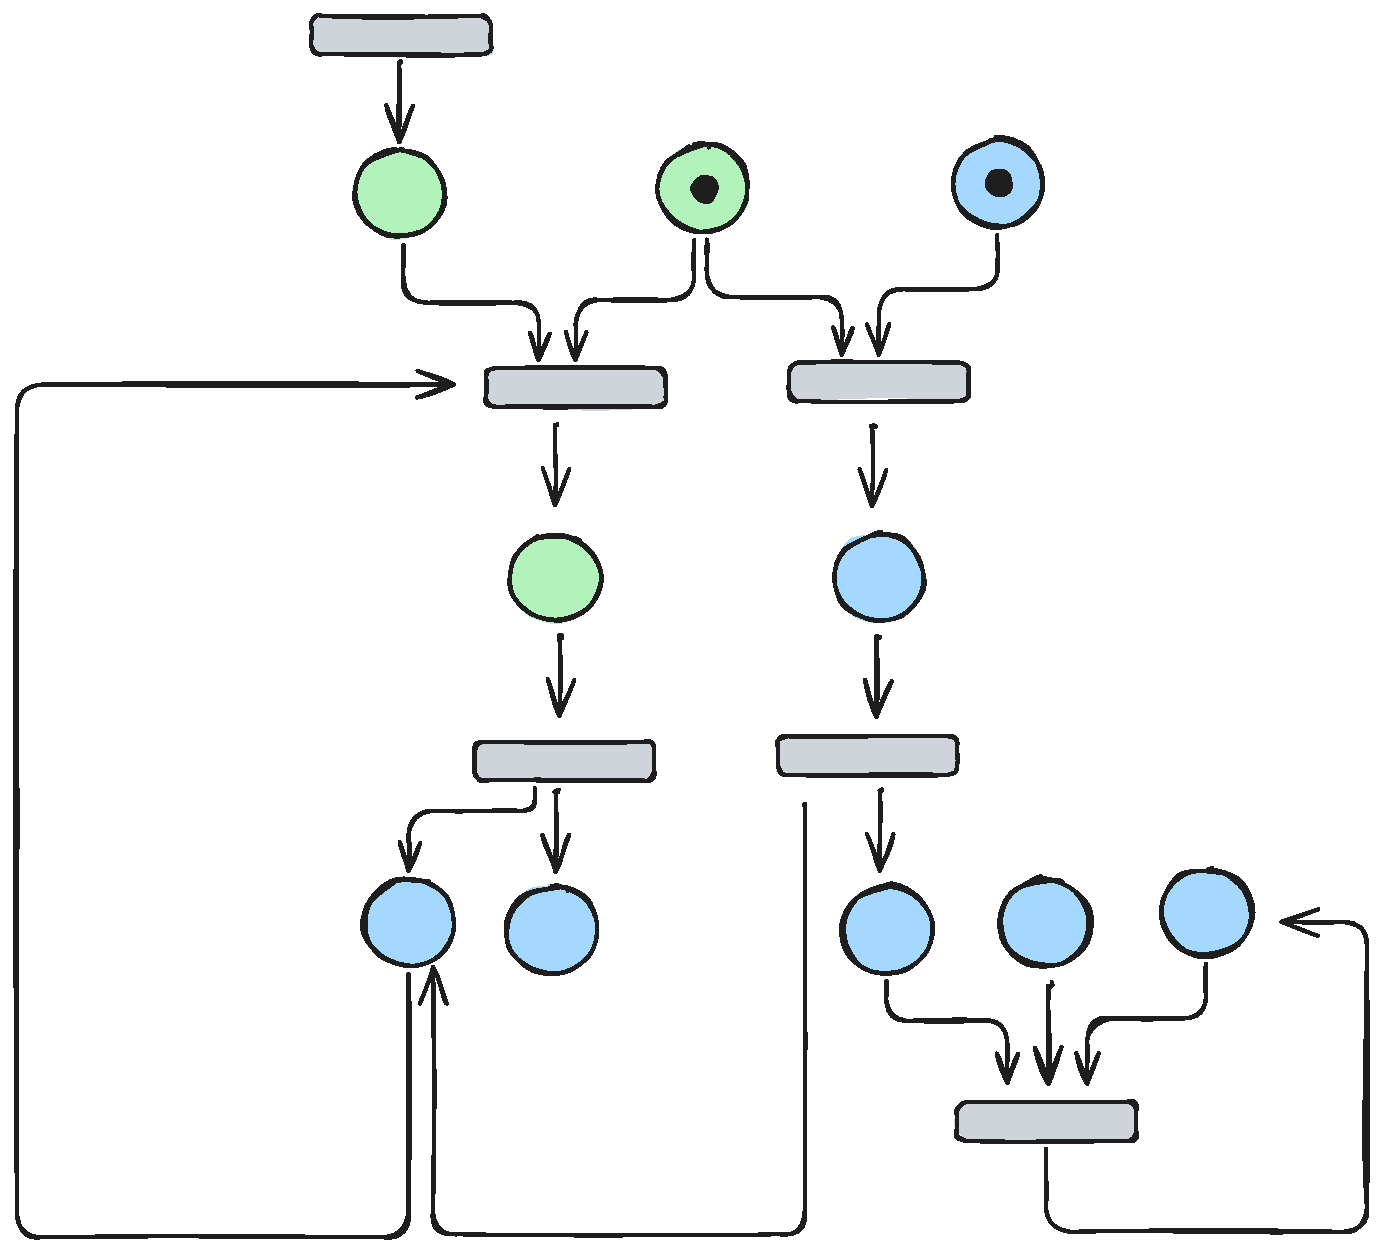
\includegraphics[width=\textwidth]{plots/bidirectional_pruning_step_a_updated.pdf}
		\caption{Step 0: initial Petri net, before pruning.}
		\label{fig:step:a}
	\end{subfigure}\hfill
	\begin{subfigure}[b]{0.45\textwidth}
		\centering
		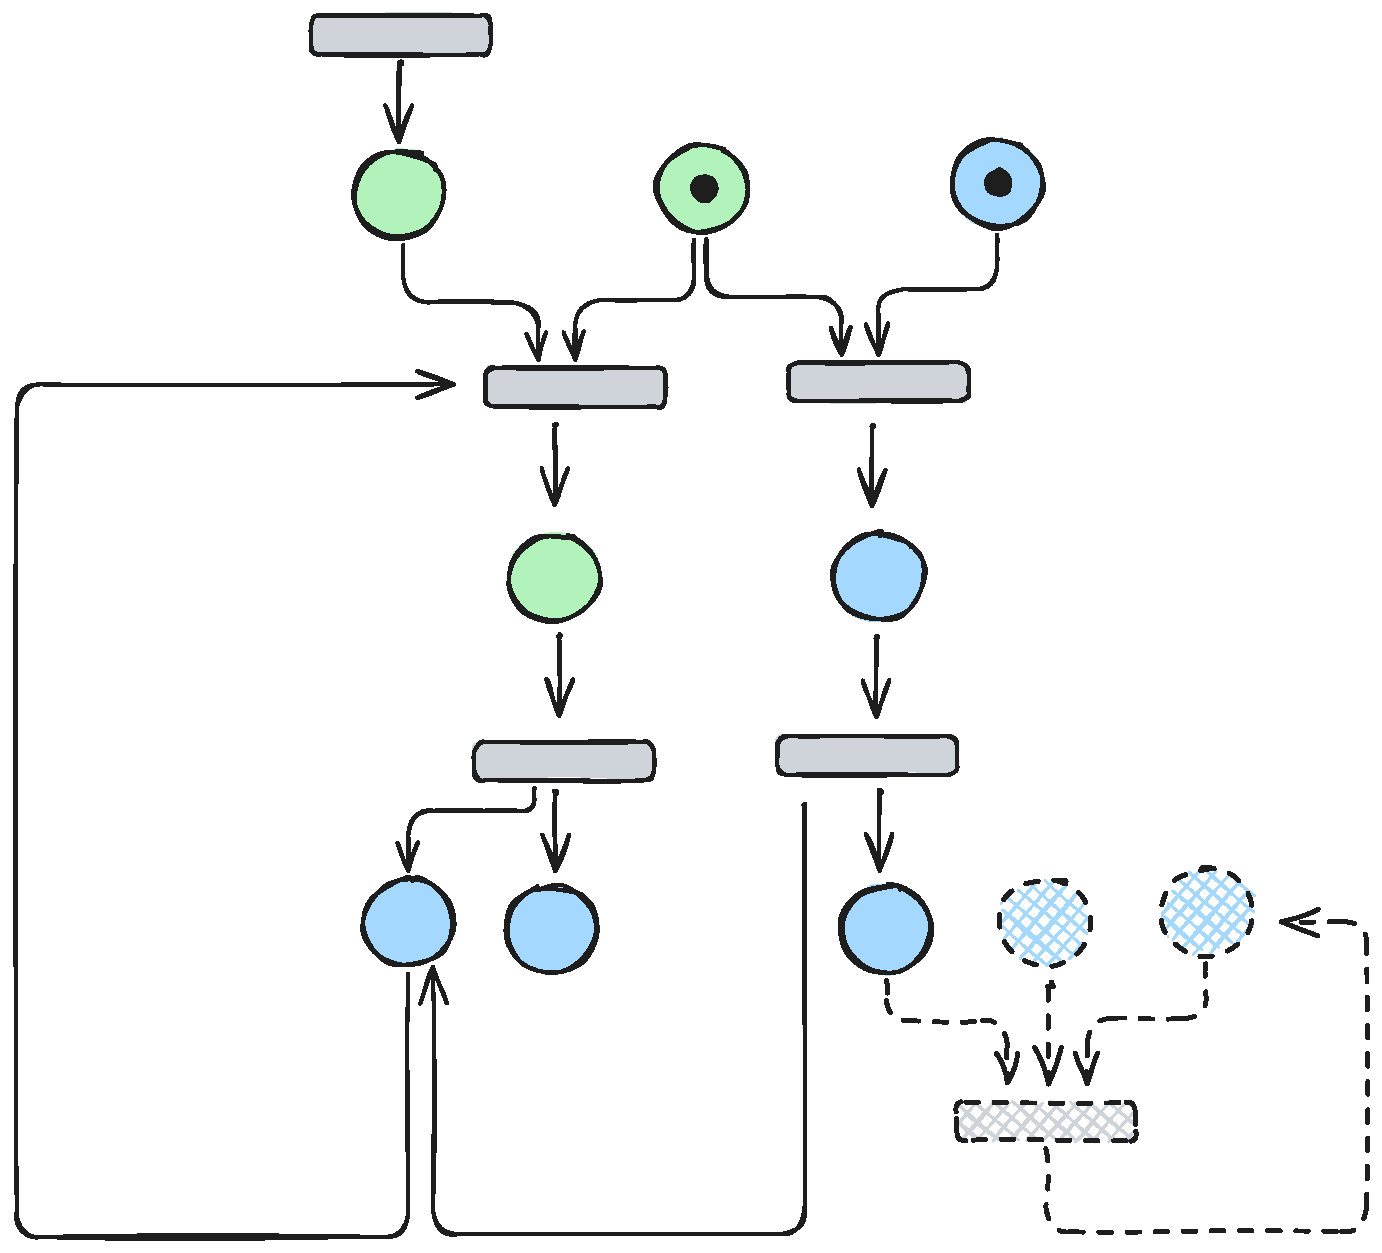
\includegraphics[width=\textwidth]{plots/bidirectional_pruning_step_b_updated.pdf}
		\caption{Step 1: first forward pass.}
		\label{fig:step:b}
	\end{subfigure}
	
	\vspace{1em}
	
	% Bottom row: (c), (d), and (e) matching (d)’s height
	\begin{subfigure}[b]{0.30\textwidth}
		\centering
		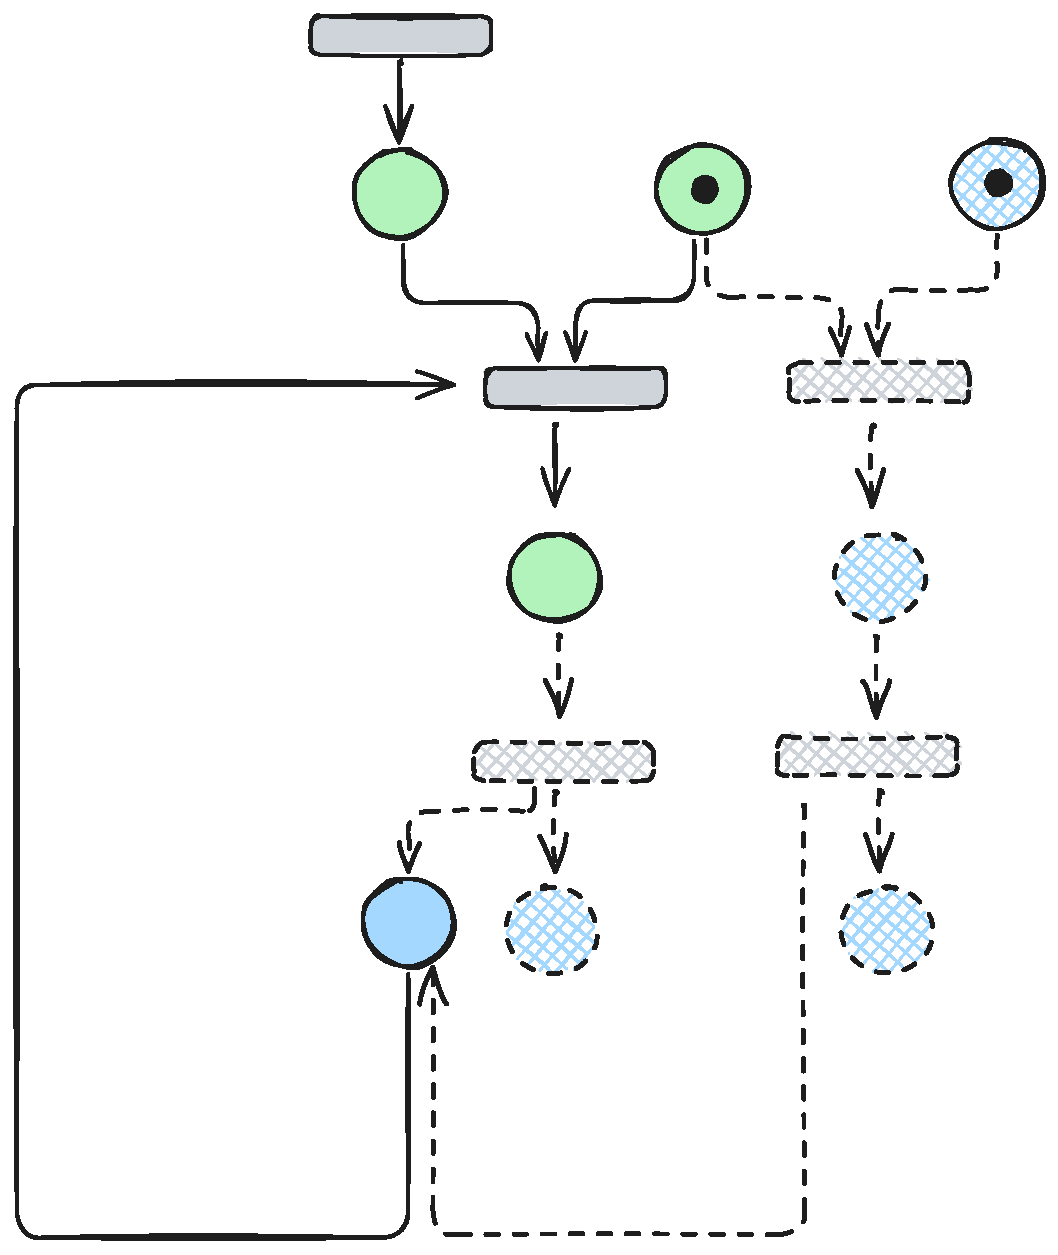
\includegraphics[width=\textwidth]{plots/bidirectional_pruning_step_c_updated.pdf}
		\caption{Step 2: first backward pass.}
		\label{fig:step:c}
	\end{subfigure}\hfill
	\begin{subfigure}[b]{0.23\textwidth}
		\centering
		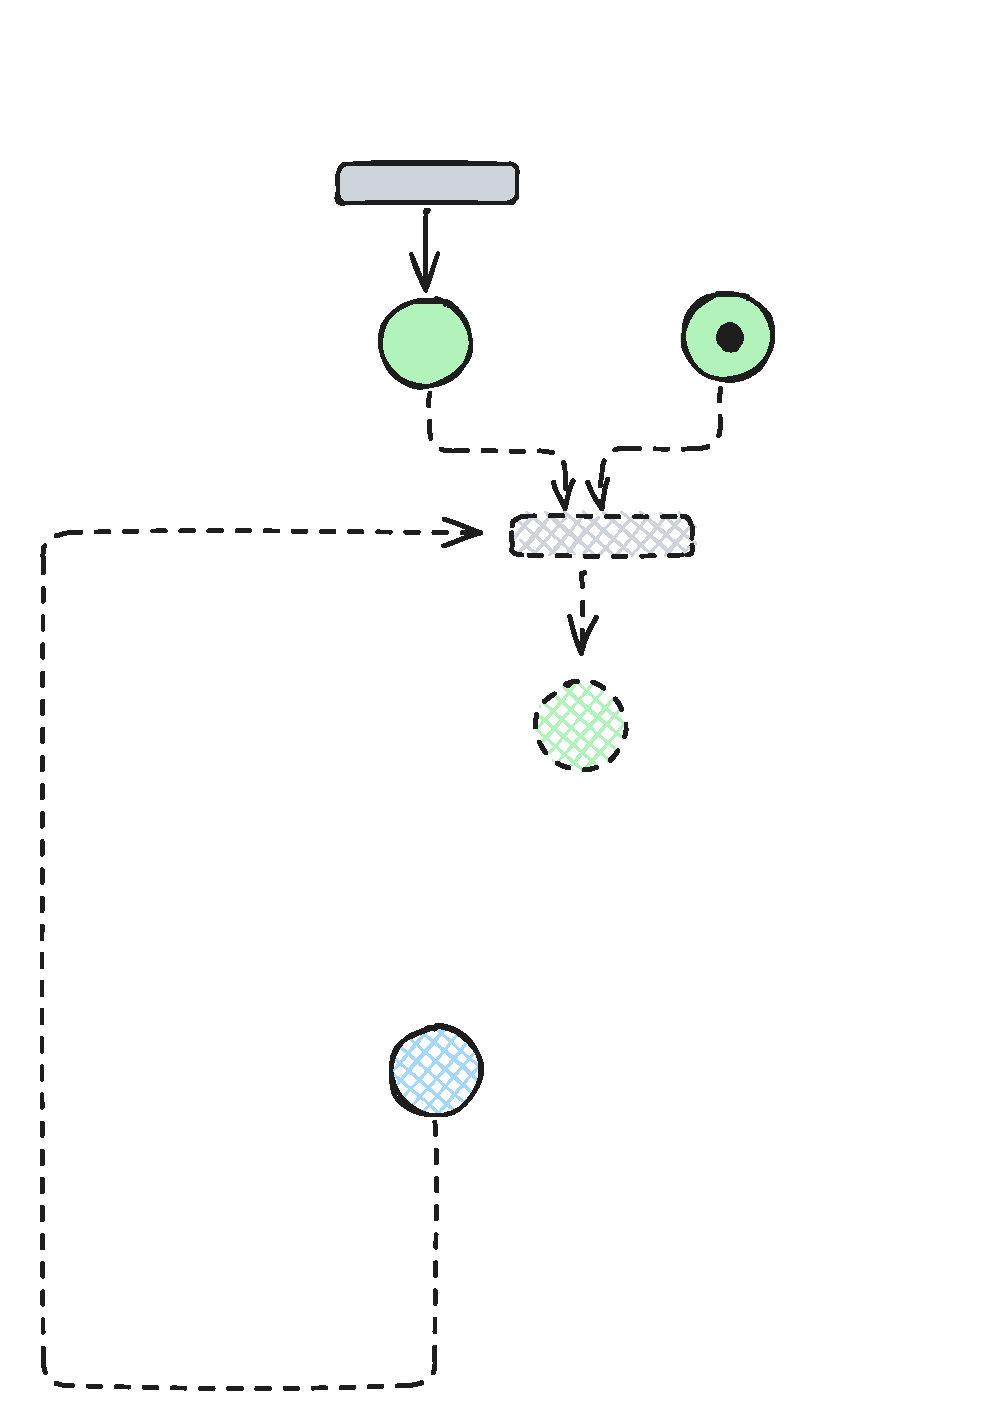
\includegraphics[width=\textwidth]{plots/bidirectional_pruning_step_d_updated_2.pdf}
		\caption{Step 3: second forward pass.}
		\label{fig:step:d}
	\end{subfigure}\hfill
	% <-- three-arg form: [vpos][total height][inner vpos]
	\begin{subfigure}[b][\subfigheight][b]{0.23\textwidth}
		\centering
		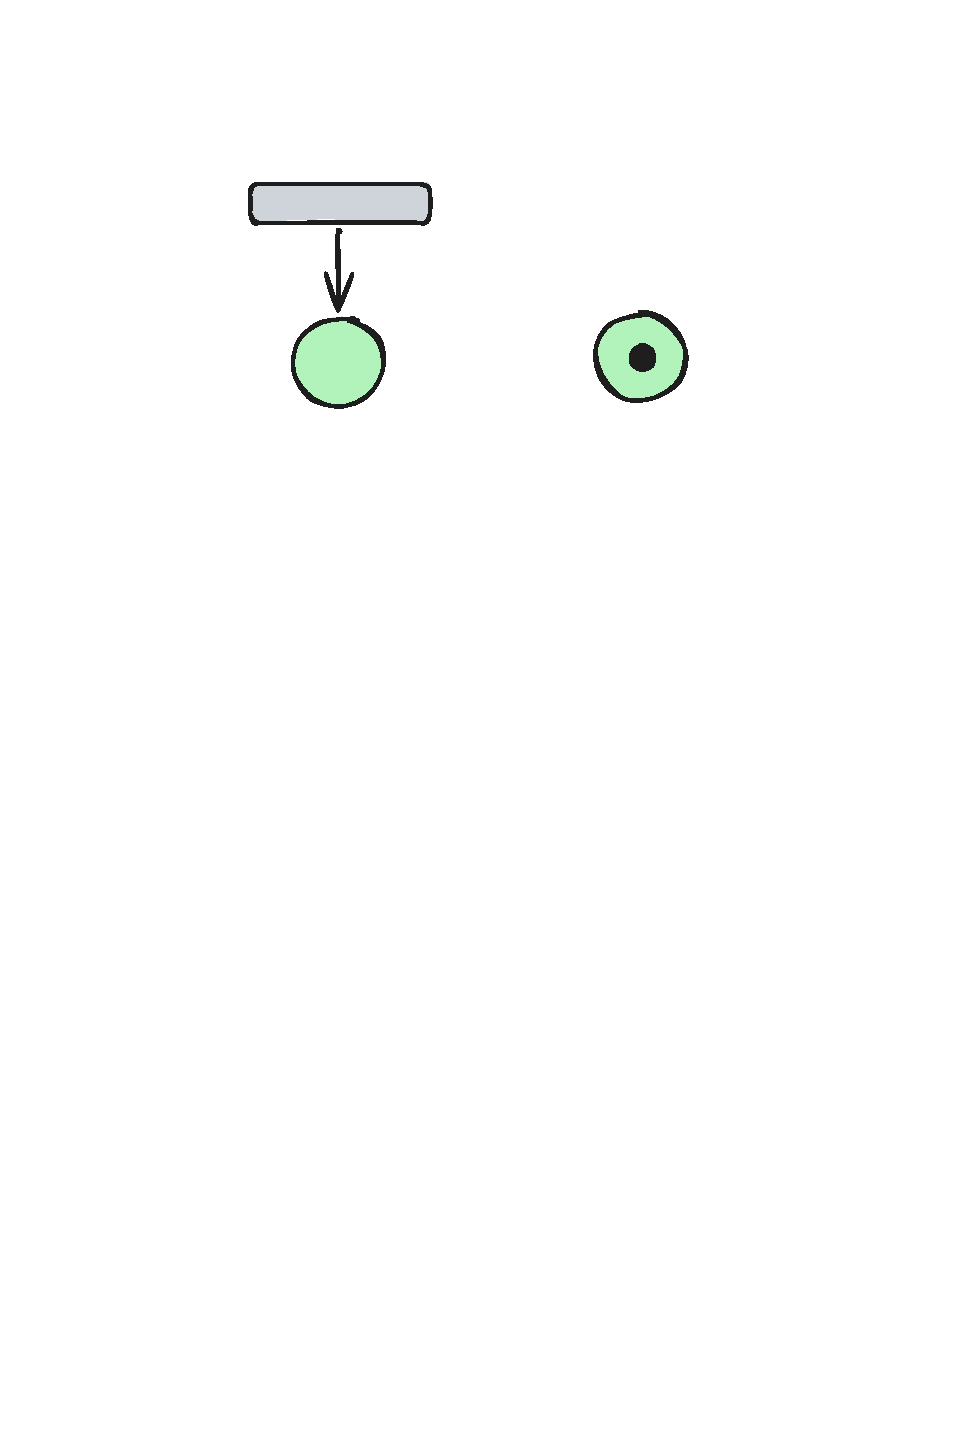
\includegraphics[width=\textwidth]{plots/bidirectional_pruning_step_e_updated_2.pdf}
		\caption{Step 4: final Petri net.}
		\label{fig:step:e}
	\end{subfigure}
	
	\caption{A Petri net after three rounds of bidirectional pruning: two forward passes and one backward pass. Black dots represent initial token markings; green places represent places that are allowed to be reachable in our constraints (i.e., aren't fixed to zero tokens in the final marking). Dashed shapes represent places and transitions that are identified as removable in the current iteration, and will be removed after it ends.}
	\label{fig:bidirectional_pruning}
\end{figure}

%\newpage

%\newpage

\section{Proof of Inductive Invariant}
\label{appendix:InductiveInvariantExample}


\begin{proof}
	
Define the predicate
\[
\begin{aligned}
	I(P_{1},\dots,P_{8})
	:={}&
		(P_{1},\textcolor{black}{P_{2}},\textcolor{black}{P_{3}},P_{4},P_{5},P_{6},\textcolor{black}{P_{7}},\textcolor{black}{P_{8}})
		\;\mapsto\;\\
		&\quad
		\exists\,e_{0},\dots,e_{5}\ge0.\;
		\Bigl(
		e_{2}-e_{1}+\textcolor{black}{P_{3}}-1=0\;\land\;
		e_{2}+P_{1}-e_{5}=0\;\land\;
		P_{5}-e_{1}+e_{4}=0\;\land\\
		&\qquad\quad
		-\,e_{4}+\textcolor{black}{P_{7}}=0\;\land\;
		P_{6}+e_{3}-e_{0}=0\;\land\;
		\textcolor{black}{P_{8}}-e_{3}=0\;\land\\
		&\qquad\quad
		-\,e_{2}+e_{1}+e_{0}+P_{4}=0\;\land\;
		-\,e_{2}+e_{1}+\textcolor{black}{P_{2}}=0
		\Bigr)
		\;\land\;
		\bigl(P_{4}-1\ge0\;\lor\;\textcolor{black}{P_{3}}-1\ge0\bigr).
	\end{aligned}
	\]
	
	
	\medskip\noindent
	\textbf{(1) Initialization.}
	The initial marking has $P_{3}=1$ and $P_{1}=P_{2}=P_{4}=P_{5}=P_{6}=P_{7}=P_{8}=0$.
	Choose $e_{0}=\cdots=e_{5}=0$.  Then
	\[
	e_{i}\ge0,\quad
	e_{2}-e_{1}+P_{3}-1=0-0+1-1=0,\;\dots,\;-e_{2}+e_{1}+P_{2}=0,
	\]
	and 
	\[
	P_{4}-1\ge0\;\lor\;P_{3}-1\ge0
	\;=\;-1\ge0\;\lor\;0\ge0
	\;=\;\texttt{FALSE}\;\lor\;\texttt{TRUE}
	\;=\;\texttt{TRUE}.
	\]
	Thus $I$ holds initially.
	
	\medskip\noindent
	\textbf{(2) Consecution.}
	One checks for each transition $t_{k}$ of the Petri net that
	\[
	I(M)\;\Longrightarrow\;I\bigl(t_{k}(M)\bigr).
	\]
	In each case the same $(e_{0},\dots,e_{5})$ can be adjusted (per the SMT certificate) to show the eight equalities and the disjunction remain valid. See our accompanying artifact~\cite{ArtifactRepository} for generating a full proof in the standard \texttt{SMT-LIB} format.
	
	\medskip\noindent
	\textbf{(3) Refutation of the property.}
	Suppose by contradiction that both $I(P)$ and it holds that:
	\[
	\phi(P):\quad
	P_{1}=0,\;
	P_{2}\ge0,\;
	P_{3}\ge0,\;
	P_{4}=0,\;
	P_{5}=0,\;
	P_{6}=0,\;
	P_{7}=0,\;
	P_{8}\ge1.
	\] 
	
	\noindent
	From
	\[
	e_{2}-e_{1}+P_{3}-1=0
	\quad\text{and}\quad
	-e_{2}+e_{1}+P_{2}=0
	\]
	we get
	\[
	P_{2}=1-P_{3}.
	\]
	From
	\[
	P_{8}-e_{3}=0
	\quad\text{and}\quad
	P_{6}+e_{3}-e_{0}=0
	\]
	and from the assumption that $P_6=0$, we get
	\[
	e_{0}=e_{3}=P_{8}
	\].
	
	
	\noindent
	Similarly, the invariant equalities 
	$(-\,e_{2}+e_{1}+e_{0}+P_{4}=0)$ and $(	-\,e_{2}+e_{1}+\textcolor{black}{P_{2}}=0)$
	induce
	\[
	P_{2}=P_{4}+e_{0}=P_{4}+P_{8},
	\]
	thus
	\[
	P_{8}=P_2-P4=(1-P_{3})-P_{4}=1-P_{3}-0=1-P_3.
	\]
	as we also assume that $P_4=0$.


	
	
	\noindent
	But $\phi$ also gives $P_{3}\ge0$ and $P_{8}\ge1$, hence $P_{3}=0$.  
	Furthermore, as our invariant includes a conjunction with $\bigl(P_{4}-1\ge0\;\lor\;\textcolor{black}{P_{3}}-1\ge0\bigr)$. As we assume by negation that the semilinear set is reachable, then $P_4=0$; and in order for both the invariant and the property to hold, then necessarily $P_3 \ge 1$, in contradiction with $P_3=0$.
	%
	  Thus $I\land\phi$ is unsatisfiable, i.e., 
	%\[
	$
	I(P)\;\Longrightarrow\;\neg\phi(P)$
	.
	%\]
	This completes the proof that $I$ is an inductive invariant refuting the given property.
\end{proof}


%\newpage


\section{Toy Petri Net Example}
\label{appendix:toyPN}

Observe the toy Petri net in Fig.~\ref{fig:toyPN}.

\begin{figure}[H]
	\centering
	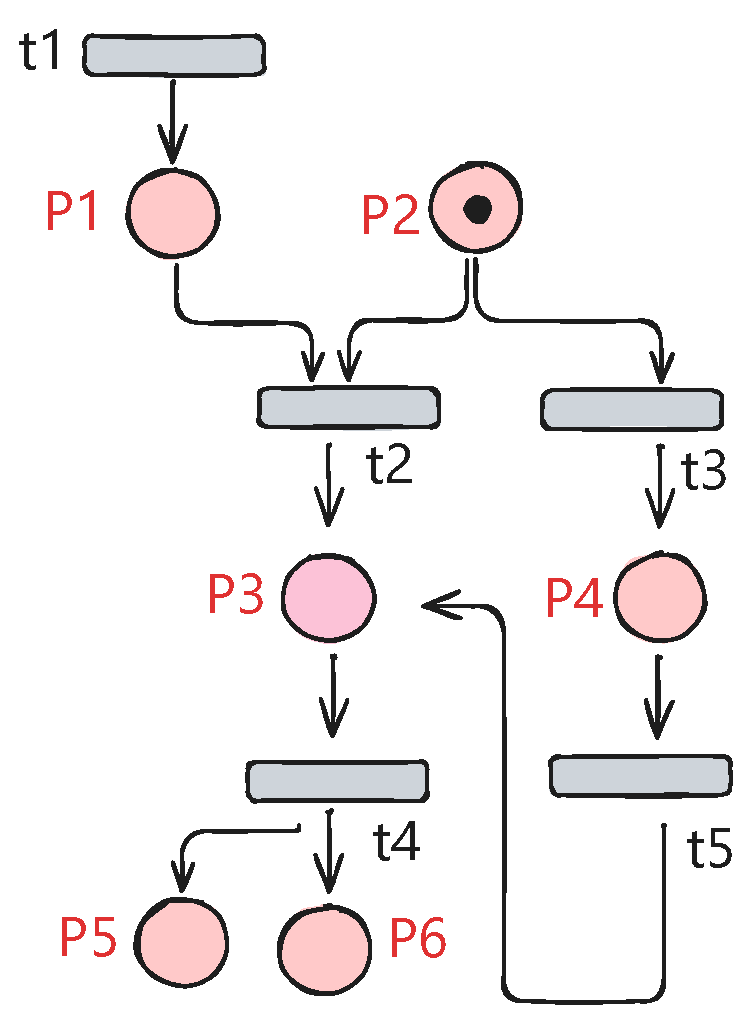
\includegraphics[width=0.3\textwidth]{plots/toy_PN_example.pdf}
	\caption{A toy Petri net.}
	\label{fig:toyPN}
\end{figure}



We formally define the net as follows:

 \(N=(P,T,\mathsf{pre},\mathsf{post},M_0)\) with
\[
P=\{P_1,P_2,P_3,P_4,P_5,P_6\},\quad
T=\{t_1,t_2,t_3,t_4,t_5\},
\]
and the mappings $\mathsf{pre}$,$\mathsf{post}$ are given as
\[
\begin{array}{c|cccccc}
	& P_1 & P_2 & P_3 & P_4 & P_5 & P_6 \\ \hline
	\mathsf{pre}(t_1)  & 0 & 0 & 0 & 0 & 0 & 0 \\
	\mathsf{post}(t_1) & 1 & 0 & 0 & 0 & 0 & 0 \\ \hline
	\mathsf{pre}(t_2)  & 1 & 1 & 0 & 0 & 0 & 0 \\
	\mathsf{post}(t_2) & 0 & 0 & 1 & 0 & 0 & 0 \\ \hline
	\mathsf{pre}(t_3)  & 0 & 1 & 0 & 0 & 0 & 0 \\
	\mathsf{post}(t_3) & 0 & 0 & 0 & 1 & 0 & 0 \\ \hline
	\mathsf{pre}(t_4)  & 0 & 0 & 1 & 0 & 0 & 0 \\
	\mathsf{post}(t_4) & 0 & 0 & 0 & 0 & 1 & 1 \\ \hline
	\mathsf{pre}(t_5)  & 0 & 0 & 0 & 1 & 0 & 0 \\
	\mathsf{post}(t_5) & 0 & 0 & 1 & 0 & 0 & 0
\end{array}
\]
The initial marking is
\[
M_0 = (0,1,0,0,0,0)^\top 
\]

Differently put, there is a single token in place $P_2$.


\begin{itemize}
	\item An examples of a \emph{reachable} marking is
	\[
	M_f = (0,0,0,0,1,1)^\top,
	\]
	reached by the firing sequence
	\[
	M_0 \xrightarrow{t_1} M_1
	\xrightarrow{t_2} M_2
	\xrightarrow{t_4} M_f,
	\]
	where
	\[
	M_1 = (1,1,0,0,0,0)^\top,
	\quad
	M_2 = (0,0,1,0,0,0)^\top.
	\]
	\item An example of a \emph{non-reachable} marking is
	\[
	M_{nr} = (0,1,1,0,0,0)^\top.
	\]
	Since producing a token at \(P_3\) (via \(t_2\)) necessarily consumes the only token in \(P_2\), and no transition replenishes \(P_2\), then it is impossible for these two places to \textit{simultaneously} hold a single token in any reachable firing. However, we note that if the initial marking was 
	
	\[
	M_0' = (0,2,0,0,0,0)^\top,
	\]
	then marking $M_{nr}$ \textit{would have} been reachable, by firing a single transition $t_1$, followed by a single transition $t_2$.
\end{itemize}






%\newpage


\section{Evaluation: Additional Results}
\label{appendix:full_results}


\begin{table}[htbp]
	\centering
	% Load the tabular from the external file:
	\begin{table}[H]
	\centering
	\begin{tabular}{l r r r r}
		\toprule
		& \multicolumn{2}{c}{Average time (ms)} 
		& \multicolumn{2}{c}{Median time (ms)} \\
		\cmidrule(lr){2-3} \cmidrule(lr){4-5}
		Category
		& \shortstack{certificate\\generation}
		& total
		& \shortstack{certificate\\generation}
		& total \\
		\midrule
		Serializable      &   2{,}273 &  25{,}531 &  1{,}178 &  2{,}238 \\
		Not serializable  &  42{,}076 &  42{,}980 &   773 &   830 \\
		All               &  39{,}613 &  52{,}858 &   797 &  2{,}080 \\
		\bottomrule
	\end{tabular}
\end{table}

	\caption{Average and median runtime. Values are rounded to the nearest integer, to reduce clutter. The \textit{total} column also includes the time for validation.}
	\label{tab:stats-summary}
\end{table}


%\todo{experiment start}
%
%
%\begin{table*}[!htbp]
%	\centering
%	\begin{minipage}[t]{0.48\textwidth}
%		\centering
%		\begin{table}[H]
	\centering
	\begin{tabular}{l c c c c}
		\toprule
		& \multicolumn{2}{c}{number of components} & \multicolumn{2}{c}{periods per component} \\
		\cmidrule(lr){2-3} \cmidrule(lr){4-5}
		& average & max & average & max \\
		\midrule
	all optimizations (baseline) & 2.91 & 22 & 1.33 & 4 \\
	without remove-redundant & 8.79 & 194 & \textbf{1.64} & 11 \\
	without generate-less & \textbf{651.41} & \textbf{20{,}484} & 1.28 & \textbf{15} \\
	without smart-kleene-order & 2.91 & 22 & 1.35 & 4 \\
  \bottomrule
	\end{tabular}
\end{table}

%		\caption{Semilinear set size reduction via optimizations.}
%		\label{tab:semilinear-size-reduction1}
%	\end{minipage}\hfill
%	\begin{minipage}[t]{0.48\textwidth}
%		\centering
%		\begin{table}[H]
	\centering
	\begin{tabular}{l r r r r}
		\toprule
		& \multicolumn{2}{c}{Average time (ms)} 
		& \multicolumn{2}{c}{Median time (ms)} \\
		\cmidrule(lr){2-3} \cmidrule(lr){4-5}
		Category
		& \shortstack{certificate\\generation}
		& total
		& \shortstack{certificate\\generation}
		& total \\
		\midrule
		Serializable      &   2{,}273 &  25{,}531 &  1{,}178 &  2{,}238 \\
		Not serializable  &  42{,}076 &  42{,}980 &   773 &   830 \\
		All               &  39{,}613 &  52{,}858 &   797 &  2{,}080 \\
		\bottomrule
	\end{tabular}
\end{table}

%		\caption{Average and median runtime. Values are rounded to the nearest integer, to reduce clutter. The \textit{total} column also includes the time for validation.}
%		\label{tab:stats-summary1}
%	\end{minipage}
%\end{table*}
%
%\todo{experiment end}


\begin{table}[H]
	\centering
	% Load the tabular from the external file:
	\begin{table}[H]
	\centering
	\small
	% increase horizontal padding between columns
	\setlength{\tabcolsep}{5pt}
	\renewcommand{\arraystretch}{0.9}
	\begin{tabular*}{\textwidth}{@{\extracolsep{\fill}}%
			p{1.5cm}   % Category
			p{1.0cm} % Benchmark
			c        % Serializable
			c c c c c c % Features
			r r       % Cert, Total
		}
		\toprule
		\multicolumn{2}{c}{\textbf{Benchmark}}
		& \textbf{Serializable}
		& \multicolumn{6}{c}{\textbf{Features}}
		& \multicolumn{2}{c}{\textbf{Runtime (ms)}} \\
		\cmidrule(lr){1-2} \cmidrule(lr){3-3} \cmidrule(lr){4-9} \cmidrule(lr){10-11}
		&
		&
		& If & While & \texttt{?} & Arith & Yield & Multi-req
		& Cert. & Total \\
		\midrule
		\multirow{7}{=}{Core expressions} & \texttt{a1.ser} & \greencmark &  & \cmark &  &  &       &   & 2 & 47 \\
		 & \texttt{a2.ser} & \xmark &  &        &  &  & \cmark &   & 280 & 296 \\
		 & \texttt{a3.ser} & \greencmark &  &        &  &  &       &   & 1 & 32 \\
		 & \texttt{a4.ser} & \greencmark &  &        &  &  & \cmark & \cmark & 637 & 1071 \\
		 & \texttt{a5.ser} & \greencmark &  & \cmark &  &  & \cmark & \cmark & 3234 & 13624 \\
		 & \texttt{a6.ser} & \xmark &  &        &  &  & \cmark & \cmark & 757 & 775 \\
		 & \texttt{a7.ser} & \greencmark & \cmark & \cmark &  &  & \cmark &   & 4 & 33 \\
		\midrule
		\multirow{4}{=}{State machines} & \texttt{b1.json} & \greencmark & \cmark &        &  &  & \cmark & \cmark & 683 & 968 \\
		 & \texttt{b2.json} & \greencmark & \cmark &        &  &  & \cmark & \cmark & 2063 & 7802 \\
		 & \texttt{b3.json} & \greencmark & \cmark &        &  &  & \cmark & \cmark & 730 & 2080 \\
		 & \texttt{b4.json} & \greencmark & \cmark &        &  &  & \cmark & \cmark & 660 & 1909 \\
		\midrule
		\multirow{8}{=}{Fred (mixed arithmetic)} & \texttt{c1.ser} & \xmark &  & \cmark &  & \cmark & \cmark & \cmark & 356195 & 356299 \\
		 & \texttt{c2.ser} & \greencmark &  & \cmark &  & \cmark & \cmark & \cmark & 9858 & 292228 \\
		 & \texttt{c3.ser} & \greencmark &  & \cmark &  & \cmark & \cmark & \cmark & 1886 & 2397 \\
		 & \texttt{c4.ser} & \greencmark &  & \cmark &  & \cmark & \cmark & \cmark & 4336 & 7193 \\
		 & \texttt{c5.ser} & \xmark &  & \cmark &  & \cmark & \cmark & \cmark & 43694 & 43735 \\
		 & \texttt{c6.ser} & \xmark &  & \cmark &  & \cmark & \cmark & \cmark & 629 & 698 \\
		 & \texttt{c7.ser} & \xmark &  & \cmark &  & \cmark & \cmark & \cmark & 797 & 875 \\
		 & \texttt{c8.ser} & \greencmark &  & \cmark &  & \cmark & \cmark & \cmark & 4357 & 8931 \\
		\midrule
		\multirow{5}{=}{Circular increment} & \texttt{d1.ser} & \greencmark & \cmark & \cmark & \cmark &  & \cmark &   & 2391 & 5373 \\
		 & \texttt{d2.ser} & \xmark & \cmark &        & \cmark &  &   \cmark &   & 628 & 731 \\
		 & \texttt{d3.ser} & \greencmark & \cmark & \cmark & \cmark &  &  \cmark &   & 2642 & 10266 \\
		 & \texttt{d4.ser} & \greencmark & \cmark & \cmark & \cmark &  &     \cmark &   & 5604 & 22249 \\
		 & \texttt{d5.ser} & \xmark & \cmark &        &  &  & \cmark &   & 495 & 554 \\
		\midrule
		\multirow{7}{=}{Concurrency \& locking loops} & \texttt{e1.ser} & \greencmark &  & \cmark &  &  & \cmark &   & 351 & 502 \\
		 & \texttt{e2.ser} & \xmark & \cmark & \cmark &  & \cmark & \cmark & \cmark & \texttt{TIMEOUT} & \texttt{TIMEOUT} \\
		 & \texttt{e3.ser} & \xmark & \cmark & \cmark &  & \cmark &   \cmark & \cmark & 24899 & 25039 \\
		 & \texttt{e4.ser} & \xmark & \cmark & \cmark &  &  \cmark &   \cmark & \cmark & 273062 & 273351 \\
		 & \texttt{e5.ser} & \greencmark & \cmark & \cmark & \cmark &  & \cmark &   & 2 & 55 \\
		 & \texttt{e6.ser} & \greencmark & \cmark & \cmark & \cmark &  & \cmark &   & 10 & 114 \\
		 & \texttt{e7.ser} & \greencmark &  & \cmark &  &  &   \cmark &   & 299 & 444 \\
		\midrule
		\multirow{9}{=}{Non-deterministic \& randomness} & \texttt{f1.ser} & \greencmark & \cmark &    \cmark    & \cmark &  & \cmark &   & 388 & 494 \\
		 & \texttt{f2.ser} & \xmark & \cmark &   \cmark     & \cmark &  & \cmark &   & 612 & 676 \\
		 & \texttt{f3.ser} & \xmark &  &        &  & \cmark &   \cmark & \cmark & 653 & 716 \\
		 & \texttt{f4.ser} & \greencmark &  &     \cmark   &  & \cmark & \cmark & \cmark & 1626 & 9515 \\
		 & \texttt{f5.ser} & \greencmark & \cmark &        & \cmark &  &       &   & 7401 & 11301 \\
		 & \texttt{f6.ser} & \xmark & \cmark &        & \cmark &  & \cmark &   & 646 & 830 \\
		 & \texttt{f7.ser} & \xmark & \cmark &        & \cmark &  &  \cmark &   & 400 & 427 \\
		 & \texttt{f8.ser} & \xmark & \cmark &        & \cmark &  &   \cmark &   & 773 & 802 \\
		 & \texttt{f9.ser} & \greencmark & \cmark &        & \cmark &  &  \cmark &   & 10 & 94 \\
		\midrule
		\multirow{7}{=}{Networking \& system protocols} & \texttt{g1.ser} & \xmark & \cmark & \cmark &  & \cmark & \cmark & \cmark & 59312 & 74539 \\
		 & \texttt{g2.ser} & \greencmark & \cmark & \cmark &  & \cmark & \cmark & \cmark & \texttt{TIMEOUT} & \texttt{TIMEOUT} \\
		 & \texttt{g3.ser} & \xmark & \cmark & \cmark & \cmark & \cmark & \cmark & \cmark & 20557 & 20954 \\
		 & \texttt{g4.ser} & \xmark & \cmark & \cmark & \cmark & \cmark & \cmark & \cmark & 6859 & 7047 \\
		 & \texttt{g5.ser} & \greencmark & \cmark & \cmark & \cmark & \cmark &   \cmark & \cmark & 3047 & 12324 \\
		 & \texttt{g6.ser} & \xmark & \cmark &        & \cmark & \cmark & \cmark &   & 8193 & 8285 \\
		 & \texttt{g7.ser} & \greencmark & \cmark &        & \cmark & \cmark &       &   & 6886 & 252752 \\
		\midrule
\bottomrule
	\end{tabular*}
\end{table}

	\caption{Overview of the benchmarks based on serializability, features, and results.}
	\label{tab:benchmarks-all}
\end{table}


\clearpage

\section{Petri Net Model Checking}
\label{appendix:smpt}


%\smallskip
%\noindent
\subsection{Petri Nets and VAS(S) Reachability}
%\label{sec:related:petri}
	
	Our work builds on both theoretical and practical advances in 
Petri net research~\cite{Mu89,Es96,Re12,EsNi24}, and specifically, \textit{Petri net model checking}~\cite{DuLaSr25,HuScReAb17,AmBeDo14,PiHaRe20,Wo18}.
	%
Moreover, numerous studies (including~\cite{LiWaChSuZh02,Zu91,AkChDaJaSa17,AnPePe13}, among others) have explored \textit{specific classes of Petri nets}, providing deeper insights into their structure, expressiveness, and verification challenges.
	%
	%The undecidability we prove 
	%for equivalence of interleavings stems from Hack’s seminal result~\cite{Ha76, 
		%HaThesis76} showing the undecidability of reachability set equivalence for 
	%Petri Nets. This undecidability originates in a series of reductions from 
	%Hilbert’s 10th problem, specifically the possibility of determining whether 
	%there exists an integer root for Diophantine equations, a problem that was 
	%later proven undecidable by Matijasēvič~\cite{Ma70}.
	%%
	%Jančar~\cite{Ja95} later provided an alternative proof to this undecidability 
	%result, by showing that Petri Nets can simulate universal (and thus 
	%undecidable) 2-counter Minsky machines~\cite{Mi67}. In addition, Jančar further 
	%strengthened the original result by proving that undecidability holds even for 
	%Petri nets with just five unbounded places.
	%
	%Furthermore, our approach also builds on 
	
	
	\medskip
	While deciding reachability in a bounded Petri net is straightforward (through exhaustive enumeration), the \textit{unbounded} case is highly nontrivial and was first solved by 
	Mayr~\cite{Ma81}, with subsequent improvements by Kosaraju~\cite{Ko82} and 
	Lambert~\cite{La92}. Recent work~\cite{CzWo22} has also established this 
	problem is \texttt{Ackermann}-complete.
	%
	These theoretical advances in Petri net reachability have given rise to a 
	plethora of practical tools, including \texttt{KReach}~\cite{DiLa20}, 
	\texttt{DICER}~\cite{XiZhLi21}, \texttt{MARCIE}~\cite{HeRoSc13}, and others. 
	%
	Our implementation leverages \texttt{SMPT} (\emph{Satisfiability Modulo Petri Nets})~\cite{AmDa23}, a state-of-the-art model checker that combines \texttt{SMT}-solving with structural invariants~\cite{AmBeDa21,AmDaHu22}.
%	 (see Appendix~\ref{appendix:smpt}). 
	%However,
	%other PN model checkers can be used as well.
	
	
\subsection{SMPT}


\texttt{SMPT} incorporates a portfolio of symbolic model checking techniques --- including Bounded Model Checking (BMC)~\cite{BiCiClZh99}, state equation reasoning~\cite{Mu77}, $k$-induction~\cite{BeDaWe18,ShSiSt20}, Property Directed Reachability (PDR)~\cite{Br11,AmDaHu22,ViGu14,BjGa15}, and random state space exploration. It acts as a front-end to an \texttt{SMT} solver (\texttt{Z3}~\cite{DeBj08}, although others can be used, e.g., \texttt{cvc}~\cite{BaCoDeHaJoKiReTi11,BaBaBrKrLaMaMoMoNiNo22}, \texttt{MathSAT}~\cite{CiGrScSe13}, etc.), while also incorporating domain-specific knowledge from Petri net theory, such as invariants and structural properties. \texttt{SMPT} has also participated in the last five editions of the \textit{Model Checking Contest} (MCC), an international competition for model-checking tools. In its most recent participation, it achieved a bronze medal and a confidence level score of  $\texttt{100\%}$, indicating it never returned an incorrect verdict~\cite{mcc:2025}.

\medskip
\texttt{SMPT} distinguishes itself from other tools in two ways that are particularly relevant to our setting and motivate its adoption. First, to the best of our knowledge, it is the only model checker for Petri nets that provides a proof of its verdict, regardless of the underlying verification technique. This means it either produces a witness trace when the property is reachable, or, more interestingly, a certificate of non-reachability~\cite{AmDaHu22} when the property is found to be unreachable.
%
The second distinguishing feature relates to our ongoing work on polyhedral reductions~\cite{AmBeDa21}, as elaborated in~\Cref{sec:discussion}.



%\newpage


\end{document}
